% errors reported by:
% Ross Kendle (1 Augugust 2010)
% Chris Grompanopoulos <grobano@gmail.com>  (22 January 2013)
% Jingguo Yao (29 May 2014, 6 June 2014)
% David Clark (7 Jan 2015)
% Kavinda Wewegama (18 Feb 2015)
% Martin Riener
% Grant Slatton (7 Mar 2015)
% Piyush Bansal (29 May 2015)

% hypermode.tex controls chapter numbering
% versions.tex controls version numbers

% Comments on a problem in concurrent programming control 
% Harris Hyman  
% January 1966   Communications of the ACM , Volume 9 Issue 1  

% VERSION HISTORY

% Version of ?? 2015
% Rewrote Section 8 (Bounded Channel and Bounded Buffer)
% Modified Section 18 (now titled "Variable Hiding and Auxiliary Variables")
% Modified Section 7.9 (Mutual Exclusion in Modern Programs)

% Version of 14 July 2012
% - Began the Principles track with Section 5 on mutual exclusion
% - Modified the proof track to reflect the fact that TLAPS's
%   SimpleArithmetic back end has been replaced by SMT backends.
% - Corrected a serious error in the Simple PlusCal Reduction Theorem
%   of Section 4.8.
% 
% Version of 12 April 2012
% - Added section 16.4 on LAMBDA, and 
%   changed example of a higher-order op in section 16.2.1. 
% - Adding Section 8 on CandidateRanking spec
% - Began a new Section 19, debugging with TLC
% - Wrote section 14.4 on the SUBSET and UNION operators
%   in the Sets chapter.

\documentclass[fleqn,leqno]{article}
\usepackage{hypertlabook}
\usepackage{graphpap}

%%%%% Added by hengxin (hfwei@nju.edu.cn) %%%%%
\usepackage{xcolor}
\usepackage{savesym}	% to resolve conflicts between packages
\savesymbol{tilde}
\usepackage{comment}	
\includecomment{ch}
\excludecomment{en}
\usepackage{xeCJK}
\newcommand{\fixme}[1]{\textcolor{purple}{FIXME: #1}}
%%%%% Added by hengxin (hfwei@nju.edu.cn) %%%%%

\makeindex

%%% Hack for showing index elements.  Will cause errors if
%%  run on entire file
%%
% \let\mmath=\ensuremath
% \def\icmd#1{\csname#1\endcsname}
% \renewcommand{\tindex}[2]{\marginpar{\red #2 (#1)}}
% \renewcommand{\ctindex}[3]{\marginpar{\red #2 (#1)}}


%\usepackage{showidx}

\pdftitle{Principles and Specification Tracks}  
\title{\bf The Principles and Specification Tracks}
\file{main}
\author{Leslie Lamport}
\date{\today}

%%%%%%%%%%%%%%%%%%%%%%%%%% Emacs macros %%%%%%%%%%%%%%%%%%%%%%%%%%%%%%%%%%% 
%&1&\vspace{-#\baselineskip}%&
%&i&\tindex{#}{}%&
%&j&\ctindex{#}{}{}%&
%&2&\begin{twocols}
%\midcol
%\verb|#|
%\end{twocols}
%&
%&q&"#"&
%&"&"#"& "
%&c&\textsc{#}& 
%&C&\ctindex{#}{@\icmd{textsc}{}}{}&
%&f&\textsf{#}& 
%&t&\texttt{#}& 
%&b&\textbf{#}& 
%&k&\kwd{#}& 
%&v&\verb|#|&  
%&p&\documentclass[fleqn,leqno]{article}
%\usepackage{hypertlabook}
%\pdftitle{}
%\begin{popup}
%\subsection*{#}
%
%\end{popup}
%\makepopup&
%&a&\documentclass[fleqn,leqno]{article}
%\usepackage{hypertlabook}
%\pdftitle{ASCII Text}
%\fixverbatim
%\begin{popup}
%\begin{verbatim*}
%#
%\end{verbatim*}
%\end{popup}
%\makeasciipopup&
%&u&\documentclass[fleqn,leqno]{article}
%\usepackage{hypertlabook}
%\pdftitle{}
%\setpopup{30}
%\begin  {document}
%#
%\end  {document}&

%&o&\ov{#}& 
%&e&\ENABLED#& 
%&U&$\mathcal{U}$#& 
%&m&\mathcal{#}&
%&g&\gssub{#}{}&
%&h&\gssubvars{#}&
%&l&\sref{main}{\xlink{main:}}{Section~\xref{main:}}&
%&r&\rd{#}&
%&F&\MF#&
%&G&\MG#& 
%&T&\tlabox{#}&
%%%%%%%%%%%%%%%%%%%%%%%%%%%%%%%%%%%%%%%%%%%%%%%%%%%%%%%

\renewcommand{\contentsname}{The \emph{Principles} and \emph{Specification} 
       Tracks\protect\target{top}}

% PROOF
\beforePfSpace{0pt}
\afterPfSpace{0pt}
\interStepSpace{0pt}

% State commands

% DieHard: [big = #1, small = #2]
\newcommand{\dhstate}[2]{\left[\!\begin{array}{l@{\,\,}c@{\,\,}c}
                        big & = & #1 \\ small & = & #2
                        \end{array}\!\right]}

%Euclid: [x = #1, y = #2, pc = #3]
\newcommand{\pestate}[3]{\left[\!\begin{array}{l@{\,\,}c@{\,\,}c}
                        x & = & #1 \\ y & = & #2 \\ pc & = & #3
                        \end{array}\!\right]}

%Alternation: [b = #1, box = #2]
\newcommand{\altstate}[2]{\left[\!\begin{array}{l@{\,\,}c@{\,\,}c}
                        b & = & #1 \\ box & = & #2
                        \end{array}\!\right]}

% Handshake : [p = #1, c = #2, box = #3, bBar = #4, boxBar = #3]
\newcommand{\hdskstate}[4]{\left[\!\begin{array}{l@{\,\,}c@{\,\,}c}
                        p & = & #1 \\ c & = & #2 \\ box & = & #3 \\
                        \ov{b} & = & #4 \\ \ov{box} & = & #3
                        \end{array}\!\right]}

% 2-step Handshake : [p = #1, c = #2, box = #3, pc = 0 :> #4 @@ 1 :> #5]
\newcommand{\hdskkstate}[5]{\left[\!\begin{array}{l@{\,\,}c@{\,\,}l}
                        p & = & #1 \\ c & = & #2 \\ box & = & #3 \\
                        pc & = & 0 :> #4\,@\!@ \\ & & 1:>#5 
                        \end{array}\!\right]}


\begin{document}

% \thispagestyle{web}
%\maketitle
\target{contents}
\showversions
\tableofcontents
\hideversions
\vfill
\newpage
\vspace*{-\baselineskip}

% Section 1: Introduction
%%%%%%%%%%%%%%%
\begin{en}
\section{Introduction}

\subsection{Concurrent Computation}

 \tindex{1}{concurrent}%
\emph{Concurrent} 
means occurring at the same time.
   \tindex{1}{concurrency}%
\emph{Concurrency} 
is the noun form of this adjective; it means the
existence of multiple things happening at the same time.

Concurrent computation means computation in which different operations
can occur concurrently.  These days, most computation is performed in
response to real-world actions---perhaps when a user moves a mouse or
clicks on a mouse button.  Concurrency in the real world means that
concurrent computation cannot be avoided.  Your computer cannot
prevent you from clicking on the mouse button while you are moving the
mouse.
\end{en}

\begin{ch}
\section{导论}

\subsection{并发计算}

 \tindex{1}{concurrent}%
 ``\emph{并发的}'' 即``同时发生的''。
作为其名词形式,
   \tindex{1}{concurrency}%
 ``\emph{并发}'' 意味着多件事情同时发生。

``并发计算''是允许不同操作并发的一种计算形式。
如今,大多数计算都是对现实世界里发生的动作的响应——比如用户移动或者点击了鼠标。
现实世界里的并发动作意味着并发计算不可避免。
当你移动鼠标的时候,你的计算机不能阻止你同时点击鼠标。
\end{ch}
%%%%%%%%%%%%%%%

%%%%%%%%%%%%%%%
\begin{en}
  \tindex{1}{parallel computation}%
  \ctindex{1}{computation!parallel}{parallel-computation}%
Parallel computation is a special kind of concurrent computation in
which different parts of a single task are performed concurrently to
speed up execution of the task.  In principle, parallelism is
avoidable because we can perform the separate parts one at a time.  It
may not be avoidable in practice because without it, executing the
task may take too long.  However, parallelism is an inherently simpler
form of concurrency because we, rather than the external world,
control when things happen.
\end{en}

\begin{ch}
  \tindex{1}{parallel computation}%
  \ctindex{1}{computation!parallel}{parallel-computation}%
并行计算是一类特殊的并发计算。
在并行计算中,为了加速完成任务,一个任务被分成多个子任务并发执行。
原则上讲,并行是可以避免的,因为我们可以按序依次执行这些子任务。
在实践中,并行或许不可避免,否则可能需要很长时间才能完成任务。
但是,即使并行(同并发一样)不可避免,究其本质而言,它只是并发的一种简单形式。
这是因为,在并行计算中,一件事情在何时发生是由我们——而非外部世界——所控制的。
\end{ch}
%%%%%%%%%%%%%%%

%%%%%%%%%%%%%%%
\begin{en}
\subsection{Modeling Computation} \label{sec:computing-devices}

Concurrent computation is computation in which different operations
can occur concurrently, but 
  \tindex{1}{computation}%
what is computation?  A simple answer is:
computation is what a computer does.  This answer is unsatisfactory
for several reasons:
\begin{itemize}
\item It's hard to define what a computer is.  Is a cell phone a
computer?  What about an MP3 player?

\item These days, computations are often performed by networks of
separate computers.

\item Computations can be performed by non-physical things---in particular,
by programs and algorithms.
\end{itemize}
A better definition is that computation is what a digital system does,
where computers, MP3 players, computer networks, programs, and
algorithms are all digital systems.  What distinguishes a digital
system is that its computation consists of a collection of discrete
events.  
\end{en}

\begin{ch}
\subsection{为计算建模} \label{sec:computing-devices}

如上所述,并发计算是允许不同操作并发的一种计算形式。
但是,
\tindex{1}{computation}%
什么是计算呢?
一个简单的答案是:计算就是一台计算机所做的那些事情。
然而,由于种种原因,这个答案不能令人满意:
\begin{itemize}
  \item 我们很难定义什么是计算机。
    一部手机是计算机吗?一部MP3播放器呢?
  \item 如今,计算通常是由多台计算机组成的网络所完成的。
  \item 计算可以由非物理设备——尤其是程序与算法——完成。
\end{itemize}
一个更好的定义是:计算就是数字系统所做的那些事情。
计算机、MP3 播放器、计算机网络、程序与算法都是数字系统。
数字系统与其它系统的区别在于它的计算是由一组离散事件构成的。
\end{ch}
%%%%%%%%%%%%%%%

%%%%%%%%%%%%%%%
\begin{en}
A pocket calculator is a digital system because its computation
consists of discrete events like the pressing of a button and the
writing of a number on its display.  But are these really discrete
events?  Changing the number shown on the display requires a few
milliseconds, during which time the display changes continuously from
showing its old value to showing its new one.  The user of the
calculator thinks of it as a single event.  The designer of the
display probably doesn't.  We consider something to be a digital
system if we think of its computation as consisting of discrete
events.  However, instead of saying that we are considering the
calculator to be a digital system, we simply say that it \emph{is}
one.  Moreover, since this hyperbook is about digital systems, I will
almost always omit the ``digital'' and simply write 
  \tindex{1}{system}%
\emph{system} to mean digital system.
\end{en}

\begin{ch}
  袖珍计算器的计算是由诸如``按键''与``在屏幕上显示数字''这样的离散事件构成的,
  所以它是一种数字系统。
  不过,这些事件真的是离散事件吗?
  改变屏幕上显示的数字需要几毫秒,
  在这段时间内,屏幕由显示旧数字连续地变成显示新数字。
  计算器的使用者会认为这种变化是一个单一事件。
  但是,屏幕的设计者很可能不这么认为。
  当我们认为某个系统的计算是由离散事件构成的时候,
  对我们来说,这个系统就是一种数字系统。
  这时,我们直接说``该系统(如计算器)是一种数字系统'',
  而不说``我们认为该系统(如计算器)是一种数字系统''。
  更进一步,由于本书的主题是数字系统,
  我将省略``数字''这一定语并使用%
    \tindex{1}{system}%
  ``\emph{系统}''指代数字系统。
\end{ch}
%%%%%%%%%%%%%%%

%%%%%%%%%%%%%%%
\begin{en}
What exactly are the discrete events of the pocket calculator system?
Is entering the number 3 on the keypad a single event?  Or are
depressing the 3 and releasing it two separate events?  A user of the
calculator probably considers entering 3 to be a single event; to the
keypad's designer, they are separate events.  
\end{en}

\begin{ch}
  袖珍计算器系统的离散事件究竟是什么?
  从键盘输入数字$3$是一个单一事件吗?
  还是说,按下按键$3$与松开按键$3$是两个不同的事件?
  计算器的使用者很可能会认为输入数字$3$是一个单一事件。
  而对键盘的设计者来说,它又包含两个不同的事件。
\end{ch}
%%%%%%%%%%%%%%%

%%%%%%%%%%%%%%%
\begin{en}
This hyperbook is not about physical systems like calculators.  It is
about 
  \ctindex{1}{system!abstract}{system-abstract}%
\emph{abstract} systems, which are abstractions of digital systems
obtained by considering their computations to consist of certain
discrete events.  The principles we study are principles of abstract
systems.
\end{en}

\begin{ch}
  本书的主题不是像计算器这样的物理系统,而是%
    \ctindex{1}{system!abstract}{system-abstract}%
  \emph{抽象}系统——那些我们认为其计算是由离散事件构成的数字系统的抽象。
  我们研究的是抽象系统的原理。
\end{ch}
%%%%%%%%%%%%%%%

%%%%%%%%%%%%%%%
\begin{en}
How do we decide what abstraction of a physical system to use?  Should
entering the number 3 be one event or two?  The answer depends on the
purpose of the abstraction.  The abstraction in which entering a
number is a single event is simpler.  However, it cannot describe the
physical possibility of depressing the 3 and then depressing the 4
before releasing the 3.  The keypad engineer cares about this
possibility, so the abstraction does not serve her purpose and she
needs separate \emph{depress} and \emph{release} events.  The user
trying to understand how to use the calculator probably doesn't care
what happens if two keys are depressed at the same time, so he will
prefer an instruction manual that adopts the simpler abstraction.

This kind of abstraction is common to all sciences.  Astronomers
studying planetary motion often use an abstraction in which a
planet is represented as a point mass.  However, that abstraction is not
satisfactory if tidal effects are important.  
\end{en}

\begin{ch}
  对一个物理系统,我们如何决定该使用什么抽象呢?
  输入数字$3$是一个事件还是包含了两个事件?
  这取决于抽象的目标。
  将输入某数字看作一个单一事件所得到的抽象比较简单。
  然而,它无法描述这样一种可能情况:
  先按下$3$,然后在松开$3$之前按下$4$。
  键盘的设计者需要考虑这种可能性,
  因此,这种抽象不能满足他们的需求,
  他们需要区分``按键''与``松键''两种事件。
  尝试理解如何使用计算器的用户很可能并不关心同时按下两个键会发生什么,
  他们更喜欢依照简单抽象写成的使用手册。

  % 这种抽象对所有学科都是共通的。
  所有学科都有这种关于抽象的问题。
  天文学家在研究行星运动时通常将行星抽象为一个质点。
  但是,如果需要考虑潮汐效应的话,这种抽象就不能满足要求了。
\end{ch}
%%%%%%%%%%%%%%%

%%%%%%%%%%%%%%%
\begin{en}
Having fewer separate events makes an abstraction simpler; having more
events allows it to more accurately represent the actual system.  We
want to use the simplest abstraction that is accurate enough.  Finding
the right abstraction is an art, but we will see that there are
principles that can guide us.
\end{en}

\begin{ch}
  包含较少事件的抽象比较简单。
  包含较多事件的抽象则可以更精确地刻画实际系统。
  我们希望使用简单而又不失精确的抽象。
  虽然如何选择正确的抽象是一门艺术,
  但是还是有一些基本原则可供遵循。
  % 但是我们将会看到一些具有引导作用的原则。
\end{ch}
%%%%%%%%%%%%%%%

%%%%%%%%%%%%%%%
\begin{en}
Having chosen an abstraction of a system, we need to decide how to
represent that abstraction.  A representation of an abstraction of a
system is called a 
  \ctindex{1}{model!system}{model-system}%
\emph{model} of the system.  There are several ways
of modeling systems.  Some take events to be primitive objects.
Others take states to be primitive, where a state is an assignment of
values to variables, with an event defined to be a transition from one
state to another.  Still others take both states and event names as
primitives, with an event being a state transition labeled by an event
name.  There is also one way of modeling systems in which the
primitive objects are sets of events.  These different kinds of models
can be used to express different classes of properties, and we will
use more than one of them.  However, the one we take as our standard
model, and the one we use most often,~is:
\begin{quote}
\textbf{The Standard Model} \  
    \ctindex{1}{model!standard}{model-standard}%
    \tindex{1}{standard model}%
An 
 \target{main:standard-model}
abstract system is described as a collection of behaviors, each
representing a possible execution of the system, where a 
  \tindex{1}{behavior}%
behavior is a
sequence of states and a 
  \tindex{1}{state}%
state is an assignment of values to
variables.
\end{quote}
In this model, an 
  \tindex{1}{event}%
event, also called a 
   \tindex{1}{step}%
\emph{step}, is the transition from one state to the next in a
behavior.  I find the standard model to be the simplest one that
scales well to descriptions of complex systems.

We model abstractions of systems.  By a \emph{system model} or a
\emph{model of a system}, I mean a model of an abstraction of a
(digital) system.
\end{en}

\begin{ch}
  选定了系统的某种抽象之后,
  我们需要决定如何表示这种抽象。
  系统的某种抽象的一种表示被称作该系统的一个%
    \ctindex{1}{model!system}{model-system}%
  \emph{模型}。
  系统建模有多种方式。
  有的将事件看作原子对象。
  有的将状态——也就是变量的赋值——看作原子对象,而将事件定义为状态之间的转换。
  还有的将状态与事件名作为原子对象,此时,事件被定义为标有事件名的状态转换。
  还有一种建模方式将事件集合看作原子对象。
  不同的模型可以表达不同的性质,我们将会接触到多种模型。
  但是,我们用得最多的是被我们称为标准模型的如下模型:
  \begin{quote}
    \textbf{标准模型} \  
      \ctindex{1}{model!standard}{model-standard}%
      \tindex{1}{standard model}%
    一个%
      \target{main:standard-model}%
    抽象系统被描述为一组(系统)行为,其中每个(系统)行为代表系统的一次可能执行。
    一个(系统)%
      \tindex{1}{behavior}%
    行为是一个状态序列,
    而一个%
      \tindex{1}{state}%
    状态则是一种变量赋值。
  \end{quote}
  在该模型中,%
    \tindex{1}{event}%
  事件,或者称%
    \tindex{1}{step}%
  \emph{步},
  被定义为系统行为中的状态转换。
  我发现上述标准模型是所有能够很好地扩展到复杂系统的模型中最简单的一种模型。

  我们为系统的某种抽象建立模型。
  我们用\emph{系统模型}(或者\emph{某系统的某个模型})
  表示为(数字)系统的某种抽象建立的模型。
\end{ch}
%%%%%%%%%%%%%%%

% I will usually omit the ``abstract'' and write simply \emph{system} to
% mean an abstraction of a digital system.  Moreover, when using the
% standard model, I will generally omit the ``model'' and let
% \emph{system} mean the standard model of an abstraction of a digital
% system.  However, it is important to remember that modeling a real
% system means abstracting---that is, choosing what aspects of the
% system we are describing and what aspects we are ignoring.  We cannot
% find an error in a program or in a system design that is not
% represented in our abstraction.  Never confuse the map with the
% territory.

\tindex{1}{specification}%
\vspace{-\baselineskip}
\subsection{Specification}    
A \emph{specification} 
is a description of a system model.  A
\emph{formal} specification is one that is written in a precisely
defined language.  I will use the term \emph{system specification} (or
\emph{specification of a system}) to mean a specification of a system
model.  

A system specification is a specification of a model of an abstraction
of a system.  It is quite removed from an actual system.  Why should
we write such a specification?

A specification is like a 
  \tindex{1}{blueprint}%
blueprint.  A blueprint is far removed from a building.  It is a sheet
of paper with writing on it, while a building is made of steel and
concrete.  There is no need to explain why we draw blueprints of
buildings.  However, it's worth pointing out that a blueprint is
useful in large part because it is so far removed from the building it
is describing.  If you want to know how many square feet of office
space the building has, it is easier to use a blueprint than to
measure the building.  It is very much easier if the blueprint was
drawn with a computer program that can automatically calculate such
things.

No one constructs a large building without first drawing blueprints of
it.  We should not build a complex system without first specifying it.
People will give many reasons why writing a specification of a
system is a waste of time:
\begin{itemize}
\item You can't automatically generate code or circuit diagrams from
the specification.

\item You (usually) can't verify that the code or circuit diagrams
correctly implement the specification.

\item While building the system, you can discover problems that
require changing what you want the system to do.  This leads to the
specification not describing the actual system.
\end{itemize}
You can find the answers to such arguments by translating them into
the corresponding ones for not drawing blueprints.

Blueprints are most useful when drawn before the building is
constructed, so they can guide its construction.  However, they are
sometimes drawn afterwards---for example, before remodeling an old
building whose blueprints have been lost.  System specifications are
also most useful before the system is built.  However, they are also
written afterwards to understand what the system does---perhaps to
look for errors or because the system needs to be modified.

A formal specification is like a detailed blueprint; an informal
specification is like a rough design sketch.  A sketch may suffice for
a small construction project such as adding a skylight or a door to a
house; an informal specification may suffice for a simple system model.
The main advantage of writing a formal specification is that you can
apply tools to check it for errors.  This hyperbook teaches you how to
write formal specifications and how to check them.  Learning to write
formal specifications will help you to write informal ones.

% From now on, I will write \emph{specification} to mean \emph{formal
% specification}.

\subsection{Systems and Languages}

A formal specification must be written in a precisely defined
language.  What language or languages should we use?

A common belief is that a system specification is most useful if 
written in a language that resembles the one in which the system is to
be implemented.  If we're specifying a program, the specification
language should look like a programming language.  By this reasoning,
if we construct a building out of bricks, the blueprints should be
made of brick.

A specification language is for describing models of abstractions of
digital systems.  Most scientists and engineers have settled on a
common informal language for describing models of abstractions of
non-digital systems: the language of mathematics.  Mathematics is the
simplest and most expressive language I know for describing digital
systems as well.  

Although mathematics is simple, the education of programmers and
computer scientists (at least in the United States) has made them
afraid of it.  Fortunately, the math that we need for writing
specifications is quite elementary.  I learned most of it in high
school; you should have learned most of it by the end of your first or
second year of university.  What you need to understand are the
elementary concepts of sets, functions, and simple logic.  You should
not only understand them, but they should be as natural to you as
simple arithmetic.  If you are not already comfortable with these
concepts, I hope that you will be after reading and writing
specifications.

Although mathematics is simple, we are fallible.  It's easy to make a
mistake when writing mathematical formulas.  It is almost as hard to
get a formula right the first time as it is to write a program that
works the first time you run it.  For them to be checked with tools,
our mathematical specifications must be formal ones.  There is no
commonly accepted formal language for writing mathematics, so I had to
design my own specification language: \tlaplus.

The \tlaplus\ language has some 
   \tindex{1}{ordinary math}%
   \ctindex{1}{math!ordinary}{math-ordinary}%
\popref{tla-vs-math}{notations and concepts that are not ordinary
math}, but you needn't worry about them now.  You'll quickly get used
to the notations, and the new concepts are either ``hidden beneath the
covers'', or else they are used mainly for advanced applications.

Although mathematics is simple and elegant, it has two disadvantages:
\begin{itemize}
\item For many algorithms, informal specifications written in
pseudo-code are simpler than ones written in mathematics.

\item Most people are not used to reading mathematical specifications
of systems; they would prefer specifications that look more like
programs.
\end{itemize}
\target{main:pluscal}%
PlusCal 
  \tindex{1}{PlusCal}%
is a language for writing formal specifications of algorithms.
It resembles a very simple programming language, except that any
\tlaplus\ expression can be used as an expression in a PlusCal
algorithm.  This makes PlusCal infinitely more expressive than any
programming language.  An algorithm written in PlusCal is translated
(compiled) into a \tlaplus\ specification that can be checked with the
\tlaplus\ tools.

PlusCal is more convenient than \tlaplus\ for describing the flow of
control in an algorithm.  This generally makes it better for
specifying sequential algorithms and shared-memory multiprocess
algorithms.  Control flow within a process is usually not important in
specifications of distributed algorithms, and the greater
expressiveness of \tlaplus\ makes it better for these algorithms.
However, \tlaplus\ is usually not much better, and the PlusCal version
may be preferable for people less comfortable with mathematics.  
Most of the algorithms in this hyperbook are written in PlusCal.

Reasoning means mathematics, so if you want to prove something about a
model of a system, you should use a \tlaplus\ specification.  PlusCal
was designed so the \tlaplus\ translation of an algorithm is 
straightforward and easy to understand.  Reasoning about the
translation is quite practical.


% Section 2: The One-Bit Clock
%%%%%%%%%%%%%%%
\begin{en}
\newpage
 \tindex{1}{One-Bit Clock}%
 \ctindex{1}{Clock!One-Bit}{clock-one-bit}%
 \vspace{-\baselineskip}%
\btarget{sec:one-bit}\section{The One-Bit Clock}

Our first example is a clock.  We consider the simplest possible
clock: one that alternately shows the ``times'' 0 and 1.  Such a clock
controls the computer on which you are reading this, with its times
being displayed as the voltage on a wire.  A real clock should tick at
an approximately constant rate.  There is a lot to explain before we
can specify that requirement, so we are going to ignore it.  This
leaves a very simple computing device that just alternates between two
states: the state in which the clock displays 0 and the state in which
it displays~1.
\end{en}

\begin{ch}
\newpage
 \tindex{1}{One-Bit Clock}%
 \ctindex{1}{Clock!One-Bit}{clock-one-bit}%
 \vspace{-\baselineskip}%
\btarget{sec:one-bit}\section{单比特时钟}

我们考虑的第一个例子是一个尽可能简单的时钟:它交替显示``时间''0与1。
这类时钟控制着你正用于阅读本书的计算机,它的``时间''表现为电缆上的电压。
真实的时钟应该基本保持匀速行走。
我们忽略这种需求,因为如果要描述它,我们还需要解释很多事情。
% 要想描述这个需求,我们还需要解释很多事情,所以我们忽略它。
这样一来,我们只需要考虑一个在两种状态之间交替的非常简单的计算设备:
一个状态显示0,另一个状态显示1。
\end{ch}
%%%%%%%%%%%%%%%

%%%%%%%%%%%%%%%
\begin{en}
This may seem a strange example to choose because it has no
concurrency.  The clock does only one thing at a time.  A system can
do any number of things at a time.  \emph{One} is a simple special
case of \emph{any number}, and it's a good place to begin.  Learning
to specify sequential systems in \tlaplus\ teaches most of what you
need to know to specify concurrent systems.
\end{en}

\begin{ch}
  这似乎是个奇怪的例子,因为它不涉及并发。
  这个时钟一次只做一件事。
  在同一时刻,一个系统可以做任意多件事。
  \emph{一}是\emph{任意多}的简单的特殊情况,这是一个好的起点。
  学习使用 \tlaplus\ 描述顺序系统能让我们掌握描述并发系统所需的大多数知识。
\end{ch}
%%%%%%%%%%%%%%%


%%%%%%%%%%%%%%%
\begin{en}
\subsection{The Clock's Behaviors} \label{sec2.1}

We use the standard model to represent the clock.  This means that a
possible execution of the clock is represented by a 
  \tindex{2}{behavior}%
behavior, which is
a sequence of states, and a 
  \tindex{2}{state}%
state is an assignment of values to variables.  We model the clock
with a single variable $b$ that represents the clock ``face'', where
the assignment of 0 to $b$ represents the clock displaying 0, and the
assignment of 1 to $b$ represents its displaying 1.  We describe the
state that assigns the value 0 to $b$ by the formula $b=0$, and
similarly for $b=1$.
\end{en}

\begin{ch}
\subsection{时钟的行为} \label{sec2.1}

我们使用标准模型建模时钟。
也就是说,时钟的一次可能执行表示为一个%
  \tindex{2}{behavior}%
行为。
一个行为是一个状态序列,而一个%
  \tindex{2}{state}%
状态则是对变量的一种赋值。
我们用一个变量$b$表示``钟面'':
$b$赋值为0表示时钟显示0,赋值为1表示时钟显示1。
我们用公式$b=0$表示``变量$b$赋值为0''这一状态;$b=1$的含义类似。
\end{ch}
%%%%%%%%%%%%%%%

%%%%%%%%%%%%%%%
\begin{en}
If we start the clock displaying 0, then we can pictorially represent
its behavior as:
 \[ %\begin{equation} \label{eq1}
   b=0 \s{.701} -> \s{.701} b=1 \s{.701} -> \s{.701} b=0 
       \s{.701} -> \s{.701} b=1 \s{.701} -> \s{.701} \cdots
 \] %\end{equation}
where ``$\cdots$'' means that the clock goes on forever the same way.
Real clocks eventually stop; the best we can expect is that they keep
running for long enough.  However, it's more convenient to consider an
ideal clock that never stops, rather than having to decide for how
long we should require it to run.  So, we describe a clock
that runs forever.
\end{en}

\begin{ch}
  如果我们让时钟从0开始,那么它的行为可以形象地描述成:
  \[ %\begin{equation} \label{eq1}
    b=0 \s{.701} -> \s{.701} b=1 \s{.701} -> \s{.701} b=0 
        \s{.701} -> \s{.701} b=1 \s{.701} -> \s{.701} \cdots
  \] %\end{equation}
  其中,``$\cdots$''表示时钟永不停歇。
  真实的时钟总会停下来;我们只能期望它运行的时间足够长。
  但是,考虑一个理想的永不停歇的时钟更为方便,
  而不必决定它究竟需要运行多长时间。
  因此,我们描述一个永不停歇的时钟。
\end{ch}
%%%%%%%%%%%%%%%

%%%%%%%%%%%%%%%
\begin{en}
We could also let the clock start displaying 1, in which case
its behavior is
 \[ % \begin{equation} \label{eqclk1}
   b=1 \s{.701} -> \s{.701} b=0 \s{.701} -> \s{.701} b=1 
       \s{.701} -> \s{.701} b=0  \s{.701} -> \s{.701} \cdots
 \] % \end{equation}
These two are the only possible behaviors of the one-bit
clock.
\end{en}

\begin{ch}
  我们也可以让时钟从1开始,在这种情况下,它的行为如下所示:
  \[ % \begin{equation} \label{eqclk1}
    b=1 \s{.701} -> \s{.701} b=0 \s{.701} -> \s{.701} b=1 
        \s{.701} -> \s{.701} b=0  \s{.701} -> \s{.701} \cdots
  \] % \end{equation}
  以上行为是单比特时钟仅有的两种行为。
\end{ch}
%%%%%%%%%%%%%%%

\pause

%%%%%%%%%%%%%%%
\begin{en}
\noindent
%
Remember that, although I have been calling them behaviors of the
clock, what I have really described are the behaviors in the standard
model of an abstraction of a real clock.  The display of a clock moves
continuously from one value to the next.  In a digital clock, the
transition may be too fast for us to see the intermediate values; but
they are there.  We are specifying an abstraction of the clock in
which these continuous changes are represented by discrete steps
(state changes).
\end{en}

\begin{ch}
  需要记住的是,尽管我们一直在使用``时钟的行为''这一说法,
  实际上,我们所描述的是``真实时钟的某种抽象的标准模型的行为''。
  真实时钟的钟面从一个值连续地变换成下一个值。
  虽然,在数字时钟里,这种变换可能发生得太快,以至于我们看不到中间值,
  但是它们是客观存在的。
  在我们所描述的时钟抽象里,这种连续的变换被表示为离散的步骤(状态变化)。
\end{ch}
%%%%%%%%%%%%%%%

% It may seem strange to call the ticking of a clock a computation.  We
% usually think of a computation as something that stops after producing
% a result---perhaps the first million digits of $\pi$.  But by that
% definition, our computers do very little computing.  We use them
% mostly for reading email, listening to music, and other ongoing tasks.
% What our one-bit clock does is typical of today's computations; it's
% just a lot simpler.
% 
% The term \emph{computation} is not very descriptive of what today's
% digital devices do.  I will therefore abandon it and use
% \emph{behavior} instead.  A computing device is therefore specified by
% describing all its behaviors, where a behavior is a sequence of
% states.  A state is an assignment of values to some collection of
% variables.  For the simple clock, the collection consists of the
% single variable $b$.

%%%%%%%%%%%%%%%
\begin{en}
\subsection{Describing the Behaviors}
\xlabel{main:one-bit:describing}

To describe a computing device, we must describe all its possible
behaviors.  I was able to list all the possible behaviors of the
one-bit clock, but that isn't feasible for any but the simplest
computing devices.  Even displaying a single behavior of a complex
device would be hard, and most computing devices have too many
behaviors to list---often, infinitely many behaviors.
\end{en}

\begin{ch}
  \subsection{描述行为}
  \xlabel{main:one-bit:describing}
  要描述一个计算设备,需要描述它的所有可能行为。
  我能够枚举单比特时钟的所有可能行为,
  但是枚举对于稍显复杂的计算设备就不可行了。
  有时,仅仅是展示复杂计算设备的单个行为都是困难的,
  更何况大多数计算设备的行为多到不胜枚举——通常是无穷多的。
\end{ch}
%%%%%%%%%%%%%%%

%%%%%%%%%%%%%%%
\begin{en}
If we look beyond their syntax, we find that practical languages for
describing computing devices specify two things:
\begin{itemize}
\item The possible initial states.

\item The possible 
  \tindex{2}{step}%
steps.  (Remember that a step is a transition from one state to the
next.)
\end{itemize}
For example, here's how the one-bit clock might be
described in a (nonexistent) programming language.
\begin{program}
\kwd{variable} $b$: \s{-.6}0, 1; \V{.3}
\kwd{while} (\kwd{true}) \{ \kwd{if} ($b=0$) $b$ := 1 
                          \kwd{else} $b$ := 0; \} 
\end{program}
The first line says that the possible initial states are $b=0$ and
$b=1$.  The second line says that if $b$ equals 0, then in the next
state it equals 1; and if it equals 1, then in the next state it
equals~0.
\end{en}

\begin{ch}
  \fixme{跳出语法层面,我们发现,要描述计算设备,一门语言需要指明以下两点:}
  \begin{itemize}
    \item 所有可能的初始状态。
    \item 所有可能的%
	\tindex{2}{step}%
	步骤。(\emph{步}即状态转换。)
  \end{itemize}
  例如,使用某种(假想的)编程语言,单比特时钟可以描述如下:
  \begin{program}
  \kwd{variable} $b$: \s{-.6}0, 1; \V{.3}
  \kwd{while} (\kwd{true}) \{ \kwd{if} ($b=0$) $b$ := 1 
			    \kwd{else} $b$ := 0; \} 
  \end{program}
  第一行指明可能的初始状态是$b=0$或$b=1$。
  第二行指明如果$b$当前为0,那么在下一个状态$b$为1;
  如果$b$当前为1,那么在下一个状态$b$为0。
\end{ch}
%%%%%%%%%%%%%%%

%%%%%%%%%%%%%%%
\begin{en}
Instead of inventing a whole new language for describing initial
states and possible next states, we will do it with mathematics.  We
do this using the Boolean operators $\land$ and $\lor$.  If you are
not as familiar with these operators of simple logic as you are with
the operators $+$ and $-$ of arithmetic, you should
\target{andor}\textsf{\rref{math}{mathlogic}{detour to a discussion
of logic.}}.
\end{en}

\begin{ch}
  我们使用数学语言来描述初始状态与可能的后继状态,
  而不是发明一门全新的语言。
  我们使用布尔操作符 $\land$ 与 $\lor$。
  如果你不像熟悉算术操作符 $+$ 与 $-$ 那样熟悉这些简单的逻辑操作符,
  你应该%
  \target{andor}\textsf{\rref{math}{mathlogic}{先看一下``关于逻辑的一些讨论''}}.
\end{ch}
%%%%%%%%%%%%%%%

%%%%%%%%%%%%%%%
\begin{en}
Describing the initial states is simple; we just assert that the 
initial value of $b$ is 0 or 1.  This assertion is expressed by
the formula:
 \[ (b=0) \; \/ \; (b=1)\]
We call this formula the 
  \tindex{1}{initial predicate}%
  \ctindex{1}{predicate!initial}{predicate-initial}%
\emph{initial predicate}.
\end{en}

\begin{ch}
  初始状态易于描述。
  我们只需要断言 $b$ 的初始值是0或者1,用公式表示如下:
  \[ (b=0) \; \/ \; (b=1)\]
  我们称该公式为%
    \tindex{1}{initial predicate}%
    \ctindex{1}{predicate!initial}{predicate-initial}%
  \emph{\tlainitpredicate}。
\end{ch}
%%%%%%%%%%%%%%%

%%%%%%%%%%%%%%%
\begin{en}
To describe the possible steps, we have to write a mathematical
formula relating the values of $b$ in two states: the first state of
the step and its next state.  We do this by letting $b$ mean the
value of $b$ in the first state, and 
 \ctindex{1}{+2a@\mmath{'} (prime)}{+2a}%
 \ctindex{1}{prime (\mmath{'})!of a variable}{prime-variable}%
$b'$ mean its value in the next state.  There are two possible steps:
one with $b=0$ and $b'=1$, and the other with $b=1$ and $b'=0$.  Thus,
all possible steps are described by this formula:
 \[   ((b=0) \; /\ \; (b'=1)) \; \/ \; ((b=1) \; /\ \; (b'=0)) 
 \]
Even this tiny formula is a little hard to read because of all the
parentheses.  For larger formulas with conjunctions and disjunctions,
it can get almost impossible to keep track of the parentheses.
\tlaplus\ allows us to write conjunctions and disjunctions
as lists of formulas bulleted by $/\ $ or $\/ $.  We can therefore
also write this formula as%
\marginpar{We can also write the initial predicate as\\
             \s{1}$\begin{disj}
                   b=0 \\ b=1
                   \end{disj}$ \V{.4}\popref{junct-warning}{\bf Warning.}}
 \[ \begin{disj}
    (b=0) \; /\ \; (b'=1) \\ (b=1) \; /\ \; (b'=0)
    \end{disj}
   \s{2}\mbox{or} \s{2}
%
 \begin{disj}
    \begin{conj}
    b=0 \\ b'=1
    \end{conj} \\
    \begin{conj}
    b=1 \\ b'=0
    \end{conj}
    \end{disj}
 \] 
However it is written, we usually call this formula the
  \ctindex{1}{next-state action@next-state action\icmd{target}{next-state-target}}{next-state action}%
  \ctindex{1}{next-state relation|see{\icmd{lref}{next-state-target}{next-state action}}}{next-state-rel}%
  \ctindex{1}{action!next-state}{action-next-state}%
\emph{next-state action} or sometimes the \emph{next-state relation}.
\end{en}
\begin{ch}
  要描述可能的\tlastep{},我们必须使用一个数学公式将 $b$ 
  在两个状态——\fixme{该\tlastep{}的出发状态与后继状态}——中的值联系起来。
  我们使用 $b$ 表示 $b$ 在出发状态的值,%
    \ctindex{1}{+2a@\mmath{'} (prime)}{+2a}%
    \ctindex{1}{prime (\mmath{'})!of a variable}{prime-variable}%
  $b'$ 表示 $b$ 在后继状态的值。
  有两种可能的\tlastep{}:
  一种是 $b = 0$ 且 $b' = 1$;
  另一种是 $b = 1$ 且 $b' = 0$。
  因此,所有可能的\tlastep{}可用如下公式表示:
  \[   
    ((b=0) \; /\ \; (b'=1)) \; \/ \; ((b=1) \; /\ \; (b'=0)) 
  \]
  由于括号的原因,即使这么短的公式也有点难以阅读。
  对于由合取与析取构成的更长的公式,我们几乎无法追踪其中的括号。
  \tlaplus\ 允许我们将合取与析取写成标有符号 $/\ $ 或 $\/ $ 的公式列表。
  因此,上式也可以写成:%
  \marginpar{我们也可以将\tlainitpredicate{}写成:\\
               \s{1}$\begin{disj}
                     b=0 \\ b=1
                     \end{disj}$ \V{.4}\popref{junct-warning}{\bf 警告.}}
  \[ \begin{disj}
     (b=0) \; /\ \; (b'=1) \\ (b=1) \; /\ \; (b'=0)
     \end{disj}
    \s{2}\mbox{or} \s{2}
  %
  \begin{disj}
     \begin{conj}
     b=0 \\ b'=1
     \end{conj} \\
     \begin{conj}
     b=1 \\ b'=0
     \end{conj}
     \end{disj}
  \] 
  不管写成什么形式,我们通常将该公式称为%
  \emph{\tlanextstateaction},有时也称为\emph{\tlanextstaterelation}。
\end{ch}
%%%%%%%%%%%%%%%

%%%%%%%%%%%%%%%
\begin{en}
\subsection{Writing the Specification}

Let's now turn the initial predicate and next-state action into a
\tlaplus\ specification.  
  \popref{open-new-spec}{Open a new spec}
in the 
  \tindex{1}{Toolbox}%
 \hyperref{http://research.microsoft.com/en-us/um/people/lamport/tla/toolbox.html}{}{}{\protect\tlaplus\
Toolbox}.
Name the specification and
its root module \emph{OneBitClock}.  This creates a new module file
named \texttt{OneBitClock.tla} and opens an editor on it.
\end{en}

\begin{ch}
  \subsection{编写规约}

  现在,我们将\tlainitpredicate{}与\tlanextstateaction{}写入 \tlaplus\ \tlaspec。
  在%
    \tindex{1}{Toolbox}%
  \hyperref{http://research.microsoft.com/en-us/um/people/lamport/tla/toolbox.html}{}{}{\protect\tlaplus\ \tlatoolbox}%
  里%
  \popref{open-new-spec}{打开新规约}。
  将\tlaspec{}与它的根\tlamodule{}命名为 \emph{OneBitClock}。
  这会创建一个名为 \texttt{OneBitClock.tla} 的\tlamodule{}文件,
  并打开一个编辑器。
\end{ch}
%%%%%%%%%%%%%%%

The newly created module looks something like this in the editor:
\begin{display}
\begin{verbatim}
------------------- MODULE OneBitClock --------------------

===========================================================
\* Modification History
\* Created Mon Dec 13 09:57:04 PST 2010 by jones
\end{verbatim}
\end{display}
The first line is the 
 \tindex{1}{module opening}%
 \ctindex{1}{opening!of module}{opening-of-module}%
\emph{module opening}; the last line is the
 \tindex{1}{module closing}%
 \ctindex{1}{closing!of module}{closing-of-module}%
\emph{module closing}.  All text before the opening and after the
closing is not part of the module and is ignored.  Each sequence of
\verb|-| characters in the opening and the sequence of \verb|=|
characters in the closing can be of any length greater than~3.  
The opening and closing are printed as follows:
\begin{display}
\begin{module}{OneBitClock}
\mbox{\strut}
\end{module}
\end{display}
We now assign names to our initial predicate and next-state action.  I
have traditionally called them $Init$ and $Next$.  However, we will be
defining some alternative initial predicates and next-state relations,
so let's call these $Init1$ and $Next1$.  These formulas are defined
as follows.
\begin{display}
\begin{notla}
Init1 == (b=0) \/ (b=1)
     
Next1 == \/ /\ b = 0
            /\ b' = 1
         \/ /\ b = 1
            /\ b' = 0
\end{notla}
\begin{tlatex}
\@x{ Init1\@s{4.12} \.{\defeq} ( b \.{=} 0 ) \.{\lor}
   ( b \.{=} 1 )}\ascii{OneBitClock-1}\target{init1-next1-clock}%
\par\vspace{8.0pt}%
\@x{ Next1 \.{\defeq} \.{\lor} \.{\land} b \.{=} 0}%
  \target{main:next1}%
\@x{\@s{55.94} \.{\land} b' \.{=} 1}%
\@x{\@s{44.83} \.{\lor} \.{\land} b \.{=} 1}%
\marginpar[1]{Remember that you can click on the link to the
 \textsc{ascii} version and copy the text.}%
\@x{\@s{55.94} \.{\land} b' \.{=} 0}%
\end{tlatex}
\end{display}
These two \tlaplus\ statements define $Init1$ and $Next1$ to be the
two formulas.  Thus, anywhere in the spec following the definition of
$Init1$, typing $Init1$ is completely equivalent to typing
\tlabox{((b=0)\/(b=1))}.  The symbol $\!==\!$ (typed \verb|==|) is
read \emph{is defined to equal}.

Now \popref{save-module}{save the module}, which should cause the
Toolbox to parse the module.  (If it doesn't, go to the
\popref{parser-preferences}{TLA+ Parser Preferences menu}.)  The
parser will report six errors, all complaining that $b$ is an unknown
operator.  Clicking on each error message in the \textsf{Parsing
Errors} view highlights the location of the error---in this case, the
location of the particular occurrence of $b$ that it is complaining
about.

Every symbol that appears in the module must either be a
primitive \tlaplus\ operator or else defined or declared before its
first use.  We must 
  \ctindex{1}%
   {variable declaration (tla)@variable declaration (\icmd{tlaplus})}%
   {tla-var-decl}%
  \ctindex{1}{declaration!tla variable@\icmd{tlaplus} variable}%
   {var-decl-tla}%
declare $b$ to be a variable, which we do by
inserting the following declaration at the beginning of the module,
before the definitions of $Init1$.%
    \ctindex{1}{variable@\icmd{textsc}{variable}}{variable}%
\begin{display}
\begin{twocols}
$\VARIABLE b$ %\ascii{OneBitClock-2} 
\midcol \verb|VARIABLE b|
\end{twocols}
\end{display}
Saving \marginpar{The
\raisebox{-2pt}{\scalebox{.75}{
\includegraphics{parsed-icon.jpg}}}
 icon in the lower-right corner tells you
 that the spec has no parsing errors.}
will make the errors go away.

\pause
%
\noindent
%
When talking about the 
  \target{two-meanings-of-spec}%
  \ctindex{1}{specification!two meanings of}{spec-two-meanings}%
\emph{specification} of the one-bit clock, we
can mean one of two things:
\begin{itemize}
\item The complete module.  

\item The initial predicate and next-state relation.
\end{itemize}
It is usually clear from the context which is meant.  To avoid
confusion, we can talk about the module rather than the specification
when we mean the first.  We use the term
  \tindex{1}{behavior specification}%
  \ctindex{1}{specification!behavior}{spec-behavior}%
\emph{behavior specification} to mean the second.

  \tindex{1}{pretty printing}%
  \vspace{-\baselineskip}%
\btarget{pretty-printing}\subsection{The Pretty-Printed Version of Your Spec}

In addition to the \textsc{ascii} version of the module that you edit,
the Toolbox can display a ``pretty-printed'' version.  This requires
the 
  \ctindex{1}{pdflatex@\icmd{texttt}{pdflatex}}{pdflatex}%
\texttt{pdflatex} program to be installed on your computer.
Information on doing that and on configuring the Toolbox's
pretty-printing options can be found in 
\marginpar{\rref{help}{toolbox-help}{How to find help pages in
                                     the Toolbox.}}
\helppage{spec/pretty-printing}{the relevant Toolbox help page}.

To produce a pretty-printed version of the module, click on the
\textsf{File} menu and choose \textsf{Produce PDF Version}.  The 
pretty-printed version will be displayed in a separate window within
the Toolbox, with \tlaplus\ expressions shown approximately the way
they are printed in this hyperbook.  You can switch
 \marginpar{\popref{pretty-printing-bug}{Does it do something else?}}
between the \textsc{ascii} and
pretty-printed versions by clicking either the \textsf{TLA Module} or
\textsf{PDF Viewer} tab in the top-left corner of the module's window.
Editing the \textsc{ascii} version does not automatically change the
pretty-printed version.  You need to run the
\textsf{File}\,/\,\textsf{Produce PDF Version} command again to update it.

The pretty-printed version is produced in a file
\texttt{OneBitClock.pdf} that the Toolbox puts in the same directory
as the module file \texttt{OneBitClock.tla}.  You can print that file
to get a paper version.

\subsection{Checking the Specification}

Let's now get the 
  \tindex{1}{TLC}%
TLC model checker to check this specification.
\popref{create-new-model}{Create a new model}.  This opens a 
  \ctindex{1}{model!editor}{model-editor}% 
model editor on the model.  That editor has three pages; the model is
opened to the \textsf{Model Overview} page.

Enter $Init1$ and $Next1$ in the appropriate fields as the initial
predicate and next-state relation, and \popref{run-tlc}{run TLC}\@.
TLC runs for a couple of seconds and stops, reporting no errors.  This
means that the specification is sensible.  More precisely, it means
that our specification completely determines a collection of
behaviors.

\pause

\noindent
%
Let's change the specification so it doesn't determine a collection of
behaviors.  Go to the module editor (by clicking on its tab) and
modify the definition of $Next1$ by replacing \verb|/\ b' = 0| with
\verb|/\ b' = "xyz"|.  The second disjunct allows a step starting with
$b=0$ to set $b$ (change its value) to the
\rref{math}{strings}{string} \tlastring{xyz}.  Save the module, return
to the model editor, and run TLC again.  This time it reports the
error:
\begin{widedisplay}\small \tt
Attempted to check equality of string "xyz" with non-string: 0
\end{widedisplay}
The \textsf{TLC Errors} window also shows:%
 \marginpar{You can \popref{resize-errors-view}{resize the fields of the 
\textsf{TLC Errors} view}.}
\begin{display}
\scalebox{.75}{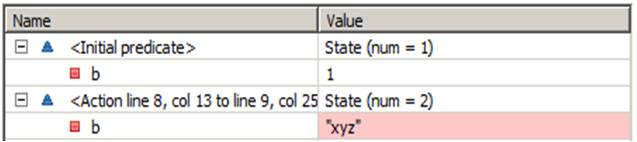
\includegraphics{OneBitClock-errortrace-1.jpg}}
\end{display}
This describes the following error trace: 
 \[ b=1 \s{.701} -> \s{.701} b = "xyz"
 \]
The trace is the beginning of a behavior that TLC was constructing
when it encountered an error.  The light-red background for the value
$"xyz"$ of $b$ indicates that it is different from the value of $b$ in
the previous state.  Double click on this line of the error trace:
\begin{display}
\scalebox{.75}{
\includegraphics{OneBitClock-errortrace-2.jpg}}
\end{display}
This raises the module editor, showing in part:
\begin{display}
\scalebox{.75}{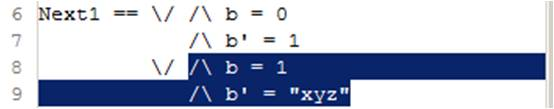
\includegraphics{OneBitClock-1.jpg}}
\end{display}
The highlighted portion is the disjunct of the next-state action $Next1$
that permits the step \,\tlabox{b=1 \, -> \, b = "xyz"}\,.

To calculate the possible next states from the state with $b="xyz"$,
TLC had to compute the value of the formula $"xyz"=0$.  (The rest of
the error message tells you that it was computing that formula in
order to evaluate the subformula $b=0$ of the definition of $Next1$.)
TLC couldn't do that because the semantics of \tlaplus\ do not
determine whether or not a string is equal to a 
  \marginpar{\popref{strings-vs-numbers}{Why shouldn't 
  \tlastring{xyz} be unequal
   to $0$?}}
number.  It could
therefore not determine if the formula $"xyz"=0$ equals \TRUE\ or
\FALSE, so it reported an error. 

Restore the original definition of $Next1$ by replacing $"xyz"$ with 0
and save the module.  Go back to the model editor and run TLC again.
It should once again find no error.

\pause
%
\noindent 
%
In the \textsf{Statistics} section of the \textsf{Model Checking
Results} page, the \textsf{State space progress} table tells you that
TLC found 2 distinct states.  The diameter of 1 means that 1 is the
largest number of steps (transitions from one state to the next) that
an execution of the one-bit clock can take before it repeats a state.

The one-bit clock is so simple there isn't much to check.  But there
is one property that we can and should check of just about any spec:
that it is 
  \tindex{1}{type correctness}%
``type correct''.  Type correctness of a \tlaplus\ specification
means that in every state of every behavior allowed by the spec, the
value of each variable is in the set of values that we expect it to
have.  For the one-bit clock, we expect the value of $b$ always to be
either 0 or 1.  This means that we expect the formula $b\in\{0,1\}$ to
be true in every state of every behavior of $b$.  If you are the least
bit unsure of what this formula means,
\target{sets}\textsf{\rref{math}{sets-intro}{detour to an introduction
to sets}}.\xlabel{main:simple-sets-return}

A formula that is true in all states of all behaviors allowed by a
spec is called an 
 \tindex{1}{invariant}%
\emph{invariant} of the spec.  Go to the
\textsf{Invariants} subsection of the \textsf{What to Check} section
of the model editor's\marginpar[.5]{Use the tabs at the top of the model
editor view to select the page.} \textsf{Model Overview} page.  Open
that subsection (by clicking on the {\bf \textsf{+}}), click on
\textsf{Add}, and enter the following formula:%
\begin{display}
\begin{twocols}
$b \in \{0, 1\}$
\midcol
\verb|b \in {0, 1}|
\end{twocols}
\end{display}
(Note that $\in$ is typed \verb|\in|.)  Click on \textsf{Finish}, and
then run TLC again on the model.  TLC should find no errors,
indicating that this formula is an invariant of the spec.

Because \tlaplus\ has no types, it has no type declarations.  As this
spec shows, there is no need for type declarations.  We don't need to
declare that $b$ is of type $\{0,1\}$ because that's implied by the
specification.  However, the reader of the spec doesn't discover that
until after she has read the definitions of the initial predicate and
next-state action.  In most real specifications, it's hard to
understand those definitions without knowing what the set of possible
values of each variable is.  It's a good idea to give the reader that
information by defining the 
 \ctindex{1}{invariant!type correctness}{inv-type-correct}%
 \ctindex{1}{type correctness!invariant}{type-correct-inv}%
type-correctness invariant in the spec,
right after the declaration of the variables.  So, let's add the
following definition to our spec, right after the declaration of $b$.
\begin{display}
\begin{twocols}
$TypeOK == b \in \{0,\,1\}$
\midcol
\verb|TypeOK == b \in {0,1}|
\end{twocols}
\end{display}
Save the spec and let's tidy up the model by using $TypeOK$ rather
than \tlabox{b \in \{0,\,1\}} as the invariant.  Go to the model
editor's \textsf{Model Overview} page, select the invariant you just
entered by clicking on it and hit \textsf{Edit} (or simply double-click on
the invariant), and replace the formula by \texttt{TypeOK}\@.  Click on
\textsf{Finish} and run TLC to check that you haven't made a mistake.

  \ctindex{1}{behavior!computing}{behavior-computing}%\
  \vspace{-\baselineskip}%
\subsection{Computing the Behaviors from the Specification}
\xlabel{sec:computing-clock-behaviors}

TLC checked that $TypeOK$ is an invariant of the specification of
the one-bit clock, meaning that it is true in all states of all
behaviors satisfying the specification.  TLC did this by computing
all possible behaviors that satisfy the initial predicate $Init1$ and
the next-state action $Next1$.  To understand how it does this, let's
see how we can do it.

We begin by computing one possible behavior.  A behavior is a sequence
of states.  To satisfy
the spec, the behavior's first state must satisfy the initial predicate
$Init1$.
A state is an assignment of values to all the spec's
variables, and this spec has only the single variable~$b$.  So to determine
a possible initial state, we must find an assignment of values to the
variable $b$ that satisfy $Init1$.  Since $Init1$ is defined to equal
 \[ (b=0) \/ (b=1) \]
there are obviously two such assignments: letting $b$ equal 0 or
letting it equal~1.  To construct one possible behavior satisfying the
spec, let's arbitrarily choose the starting state in which $b$
equals~1.  As before, we write that state as the formula $b=1$.

We next find a possible second state of the behavior.  For a behavior
to satisfy the spec, every pair of successive states must satisfy the
next-state action $Next1$, where the values of the unprimed variables
are the values assigned to them by the first state of the pair and the
values of the primed variables are the values assigned to them by the
second state of the pair.  The first state of our behavior is $b=1$.
To obtain the second state, we need to find a value for $b'$ that
satisfies $Next1$ when $b$ has the value 1.  We then let $b$ equal
that value in the second state.  To find this value, we substitute
$1$ for $b$ in $Next1$ and simplify the formula.  Recall that $Next1$
is defined to equal
 \[ \begin{disj}
    \begin{conj}
            b = 0 \\
            b' = 1
     \end{conj} \\
      \begin{conj}
         b = 1 \\
         b' = 0
     \end{conj}
    \end{disj}
 \]
We substitute 1 for $b$ and simplify as follows.
\begin{display}
\begin{tabbing}
   $\begin{disj}
    \begin{conj}
            1 = 0 \\
            b' = 1
     \end{conj} \\
      \begin{conj}
         1 = 1 \\
         b' = 0\vs{.75}
     \end{conj}
    \end{disj}$  \s{3} \=
    the formula obtained by substituting 1 for $b$ in $Next1$.\\
   $\mbox{} = \;\; \begin{disj}
    \begin{conj}
            \FALSE \\
            b' = 1
     \end{conj} \\
      \begin{conj}
         \TRUE \\
         b' = 0\vs{.75}
     \end{conj}
    \end{disj}$ \> because $\;(0=1) = \FALSE\;$ and $\;(1=1) = \TRUE$ \\
%
   $\mbox{} = \;\; \begin{disj}
         \FALSE    \\ b' = 0 
         \vs{.75}
    \end{disj}$ \> \begin{minipage}[t]{.75\textwidth}
                   because $\;\FALSE /\ F = \FALSE\;$ and 
                           $\;\TRUE /\ F = F\;$ \\
                   for any truth value $F$
                   \end{minipage} \\
%
   $\mbox{} = \;\; b'=0$ \> \begin{minipage}[t]{.6\textwidth}
                   because $\FALSE \/ F = F$ 
                   for any truth value $F$.
                   \end{minipage}
\end{tabbing}
\end{display}
This computation shows that if we substitute $1$ for $b$ in $Next1$,
then the only value we can then substitute for $b'$ that makes $Next1$
true is~0.  Hence, the second state of our behavior can only be $b=0$,
and our behavior starts with
 \[ b=1 \s{.701} -> \s{.701} b=0 \]
To find the third state of our behavior, we substitute $0$ for $b$ in
$Next1$ and find a value for $b'$ that makes $Next1$ true.  It should be
clear that the same type of calculation we just did shows that the only
possible value for $b'$ that makes $Next1$ true is~1.  (If it's not
clear, go ahead and do the calculation.)  The first three states
of our behavior therefore must be
 \[ b=1 \s{.701} -> \s{.701} b=0 \s{.701}-> \s{.701}  b=1
  \]
We could continue our calculations to find the fourth state of the
behavior, but we don't have to.  We've already seen that the only
possible state that can follow $b=1$ is $b=0$.  We can deduce
that \popref{finite-behaviors}{we must obtain the infinite behavior} 
 \[ b=1 \s{.701} -> \s{.701} b=0 \s{.701}-> \s{.701}  b=1 \s{.701} -> 
    \s{.701} b=0 \s{.701}-> \s{.701} \cdots
  \]
To find all possible behaviors, recall that the only other possible
starting state is $b=0$.  From the calculations we've already done,
we know that the only state that can follow $b=0$ is $b=1$.  We
therefore see that the only other possible behavior is
 \[ b=0 \s{.701}-> \s{.701}  b=1 \s{.701} -> \s{.701} b=0 \s{.701}-> \s{.701}  
    b=1 \s{.701} -> \s{.701} \cdots
  \]

\medskip

This example shows how we can compute all possible behaviors allowed
by a specification.  We construct as follows a
  \popref{directed-graph}{directed graph} 
$\mathcal{G}$, called the
  \ctindex{1}{graph!state}{graph-state}%
  \tindex{1}{state graph}%
  \target{main:state-graph}%
  \emph{state graph},
whose nodes are states:
\begin{enumerate}
\item We start by setting $\mathcal{G}$ to the set of all possible
initial states of behaviors, which we find by computing all possible
assignments of values to variables that make the initial predicate
true.

\item For every state $s$ in $\mathcal{G}$, we compute as follows all
possible states $t$ such that $s->t$ can be a step in a behavior.  We
substitute the values assigned to variables by $s$ for the unprimed
variables in the next-state action, and then compute all possible
assignments of values to the primed variables that make the next-state
action true.

\item For every state $t$ found in step 2: (i)~we add $t$ to $\mathcal{G}$
if it is not already in $\mathcal{G}$, and (ii)~we draw an edge from
$s$ to $t$.

\item We repeat steps 2 and 3 until no new states or edges can be
added to $\mathcal{G}$.
\end{enumerate}
If and when this process terminates, the nodes of $\mathcal{G}$
consist of all the 
  \tindex{1}{reachable state}%
  \ctindex{1}{state!reachable}{state-reachable}%
reachable states of the specifications---that is, all states that
occur in some behavior satisfying the specification.  Every behavior
satisfying the specification can be found by starting in an initial
state (found in step~1) and following a (possibly infinite) path in
$\mathcal{G}$.

\medskip

This procedure is used by TLC to compute all possible behaviors.  The
  \tindex{1}{state space progress table}%
\emph{State space progress} table in the \textsf{Statistics} section
of the \textsf{Model Checking Results} page gives the following
information about the graph $\mathcal{G}$ that it is constructing.
\begin{description}
\item[Diameter] The number of states in the longest path of
                $\mathcal{G}$ in which no state appears twice.
\item[States Found] The total number of (not necessarily distinct)
states it examined in step~1 or as successor states $t$ in step~2.

\item[Distinct States] The number of states that form the set of nodes
of $\mathcal{G}$.

\item[Queue Size] The number of states $s$ in $\mathcal{G}$ for which
step~2 has not yet been performed.
\end{description}
Of course, if the specification has an infinite number of reachable
states, this procedure will continue until $\mathcal{G}$ becomes so
large that TLC runs out of space.  However, this could take many years
because TLC keeps $\mathcal{G}$ and its queue of unexamined states on
disk when there is not enough room for them in memory.

Although TLC computes the behaviors that satisfy a specification the
same way we do, it's not nearly as smart as we are.  For example,
writing $1=b$ instead of $b=1$ in the initial predicate would make no
difference to us.  See how TLC reacts by making this change to the
definition of $Init1$ in module $OneBitClock$ and running TLC on the
model you created.  You will find that it produces the following error
report:
\begin{widedisplay} \tt
In evaluation, the identifier b is either undefined or not an operator.\\
{\darkaqua\underline{line 6, col 22 to line 6, col 22 of module OneBitClock}}.\\
The error occurred when TLC was evaluating the nested\\
expressions at the following positions:\\
0. {\darkaqua\underline{Line 6, column 22 to line 6, column 22 in OneBitClock}}
\end{widedisplay}
The underlined location indicators are links.  (They may not actually be
underlined in the Toolbox.)  Clicking on either of them jumps
to and highlights the $b$ in $1=b$.

TLC tries to find all possible initial states from the initial
predicate in a very simple-minded way.  It examines the predicate in a
linear fashion to try to find all possible assignments of values to
the variables.  When it encounters an occurrence of a variable $v$
whose value it has not yet determined, that occurrence must very
obviously determine the value of $v$.  This means that the occurrence
must be in a formula $v = e$ or $v\in e$ for some expression $e$ that
does not contain $v$.  For example, when TLC evaluated the initial
predicate
 \[ (b=0) \/ (1=b) \]
it first saw that it was a disjunction, so it examined the two
disjuncts separately.  The first disjunct, $b=0$, has the right form to
determine the value of $b$---that is, it has the form $v=e$ where $v$
is the variable $b$ and $e$ is the expression $0$.  However, when
examining the disjunct $1=b$, it first encountered the variable $b$ in
an expression that did not have the right form.  It therefore reported
that occurrence of $b$ as an error.  You can check that TLC has no
problem with the equivalent initial predicate
  \[ (b=0)\, \/ \, ((b=1) /\ (1=b))
  \]
because, when it encounters the expression $1=b$, it has already
determined the value of $b$.

\begin{aquestion}{tlc-answer-1}
What happens if you change the initial predicate to
 \[ (b=0)\, \/ \,((b=1) /\ (2=b))\]
and run TLC.
\end{aquestion}
%
These same remarks apply to the way TLC determines the possible
assignments to the primed variables from the next-state action when
performing step~2 of the procedure above.  The first time TLC
encounters a primed variable $v'$ whose value it has not yet
determined, that occurrence must be in a formula $v' = e$ or $v'\in e$
for some expression $e$ not containing $v'$.
 

\subsection{Other Ways of Writing the Behavior Specification}
\xlabel{main:one-bit:other-ways}

\rref{math}{otherops}{\textsf{If you are not intimately acquainted with the
propositional-logic operators $\Rightarrow$ (implication), $\equiv$
(equivalence), and $~$ (negation), detour here.}}\target{otherops}

\medskip

\noindent The astute reader will have noticed that the
two formulas $Init1$ and $TypeOK$, which equal $(b=0) \/ (b=1)$ and $b
\in \{0,\,1\}$, respectively, both assert that $b$ equals either 0 or
1.  In other words, these two formulas are equivalent---meaning that
the following formula equals $\TRUE$ for any value of $b$:
 \[ ((b=0) \/ (b=1)) \;\equiv\; (b \in \{0,\,1\})
 \]
%   \marginpar{\rref{math}{otherops}{Exactly what does 
%               \emph{equivalent} mean?}}  
The two formulas can be used interchangeably.
To test this, return to the Toolbox and select the \textsf{Model
Overview} page of the model editor.  Replace $Init1$ by $TypeOK$ in
the \textsf{Init} field and run TLC again.  You should find that
nothing has changed.

There are a number of different ways to write the next-state action.
This action should assert that $b'$ equals 1 if $b$ equals 0, and
equals 0 if $b$ equals 1.  Since the value of $b$ is equal to either 0
or 1 in every state of the behavior, an equivalent way to say this is
that $b'$ equals 1 if $b$ equals 0, else it equals 0.  This is expressed
by the formula $Next2$, that we define as follows.%
  \ctindex{1}{if then else@\icmd{textsc}{if}\icmd{ldots}\icmd{textsc}{then}\icmd{ldots}\icmd{textsc}{else}}{if-then-else}%
\begin{twocols}
$Next2  ==  b' = \IF b = 0 \THEN 1 \ELSE 0$
\midcol
\verb|Next2  ==  b' = IF b = 0 THEN 1 ELSE 0|
\end{twocols}
The meaning of the $\IF$\ldots$\THEN$\ldots$\ELSE\!\!\!$ construct
should be evident.

Unlike $Init1$ and $TypeOK$, the two formulas $Next1$ and $Next2$ are
not equivalent.  However, they are equivalent if $b$ equals 0 or 1.
More precisely, the following formula equals $\TRUE$ for
all values of $b$:
 \marginpar{\popref{main-impl-question}{\textsf{Why is this formula 
        true if $b$ equals 42?}}}
 \[ TypeOK \; => \; (Next1 \,\equiv\, Next2)
 \]
When used with $Init1$ as the initial predicate, both next-state
actions yield specifications for which each state of each behavior
satisfies $TypeOK$.  Hence, the truth of this formula implies that the
two specs are equivalent---meaning that they have the same set of
allowed behaviors.  Test this by copying and pasting the definition of
$Next2$ into the module (anywhere after the declaration of $b$),
saving the module, replacing $Next1$ by $Next2$ in the \textsf{Next}
field of the model, and running TLC again.

The method of writing the next-state action that I find most
elegant is to use the 
  \tindex{1}{modulus operator}% 
  \ctindex{1}{+5w@\mmath{\%} (modulus)}{+5w}%
  \rref{math}{math:modulus}{modulus operator $\%$},
where $a\,\%\, b$ is the remainder when $a$ is divided by $b$. 
Since $0\,\%\,2 = 0$, $1\,\%\,2 = 1$, and $2\,\%\,2 = 0$,
it's easy to check that, if $b$ equals 0 or 1, then $Next1$ and
$Next2$ are equivalent to the following formula.
\begin{display}
\begin{twocols}
$Next3  ==  b' = (b+1)\,\%\,2$
\midcol
\verb|Next3  ==  b' = (b + 1) % 2|
\end{twocols}
\end{display}
Add this definition to the module and save the module.  This will
generate a parsing error, informing you that the operator \,$\%$\, is
not defined.  The usual arithmetic operators, including $\,+\,$ and
$\,-\,$, are not built-in operators of \tlaplus.  Instead, they must be
imported from one of the \popref{standard-arith-modules}{standard
\protect\tlaplus\ arithmetic modules}, using an \textsc{extends} statement.
You will usually want to import the 
  \ctindex{1}{Integers module@\mmath{Integers} module}{integers-module}%
$Integers$ module, which you do
with the following statement:%
\begin{display}
\begin{twocols}
$\EXTENDS Integers$\ctindex{1}{extends@\icmd{textsc}{extends}}{extends}%
\midcol
\verb|EXTENDS Integers|
\end{twocols}
\end{display}
Add this statement to the 
beginning%
 \marginpar{\popref{extends-location}{Where can an \textsc{extends} go?}}
of the module and save the module.  Open the model editor's
\textsf{Model Overview} page, replace the next-state action $Next2$
with $Next3$, and run TLC to check this specification.

\pause

\noindent
Mathematics provides many different ways of expressing the same thing.
There are an infinite number of formulas equivalent to any given
formula.  For example, here's a formula that's equivalent to 
$Next2$.
\begin{display}
\begin{notla}
IF b = 0 THEN b' = 1
         ELSE b' = 0
\end{notla}
\begin{tlatex}
\@x{ {\IF} b \.{=} 0 \.{\THEN} b' \.{=} 1}%
\@x{\@s{35.71} \.{\ELSE} b' \.{=} 0}%
\end{tlatex}
\end{display}
As $Next1$ and $Next2$ show, even two next-state actions that are not
equivalent can yield equivalent specifications---that is,
specifications describing the same sets of behaviors.

\begin{aquestion}{logic-answer2}
Use the propositional operators $=>$ and $/\ $ to write a
next-state action that yields another equivalent
specification of the one-bit clock.
How many other next-state actions can you find that also
produce equivalent specifications?  
\end{aquestion}

\begin{aquestion}{logic-answer1}
Can inequivalent initial
predicates produce equivalent specifications?
\end{aquestion}
%
% \textsf{If you are not following the
% \emph{Principles} track and are uninterested in PlusCal, you can 
% \lref{section.\getrefnumber{sec:euclid}}{skip to Section~\ref{sec:euclid}.}}


% \subsection{Making the Spec Easier to Read and Rewrite}
% 
% \textbf{Not yet written.} Will discuss comments and the pretty-printed
% version, directing the reader to use Help if pretty-printing doesn't
% work in his Toolbox. 

% \bigskip

% \noindent
% \sref{proof}{theorems}{\textsf{To begin the Proof Track, click here.}}


\subsection{Specifying the Clock in PlusCal} \xlabel{sec:pcal-clock}

We now specify the 1-bit clock as a \lref{main:pluscal}{PlusCal} algorithm,
which means that we start learning the PlusCal language.  If at any
point you want to jump ahead, you can read the
   \hyperref{http://research.microsoft.com/en-us/um/people/lamport/tla/c-manual.pdf}{}{}{PlusCal
  language manual}.

In the Toolbox, \popref{open-new-spec}{open a new spec} and name the
specification and its root module \emph{PCalOneBitClock}.  The
algorithm is written inside a 
  \ctindex{1}{comment!multi-line}{comment-multi-line}%
  \tindex{1}{multi-line comment}%
multi-line comment, which is begun by
\verb|(*| and ended by \verb|*)|.  The easy way to create such a
comment is to put the 
  \popref{cursor}{cursor} at the left margin and type
\textsf{control+o} \textsf{control+s}.  (You can also right-click and
select \textsf{Start Boxed Comment}.)  Your file will now look about
like this.
\begin{verbatim}
-------------------------- MODULE PCalOneBitClock --------------------------

(***************************************************************************

 ***************************************************************************)
=============================================================================
\end{verbatim}
We need to choose an arbitrary name for the algorithm.  Let's call it
\emph{Clock}.  We start by typing this inside the
   comment:%
\begin{display}
\begin{twocols}
\verb|--|\textbf{algorithm} $Clock$ \{\\
\}
\midcol
\begin{verbatim}
--algorithm Clock {
}
\end{verbatim}
\end{twocols}
\end{display}
The 
  \ctindex{1}{algorithm token@\icmd{textbf}{-{}-algorithm} token}%
  {algorithm-token}%
\verb|--| in the token \verb|--|\textbf{algorithm} has no
significance; it's just a meaningless piece of required syntax that
you're otherwise unlikely to put in a comment.

The body of the algorithm appears between the curly braces \{\,\,\}.
It begins by declaring the variable $b$ and specifying its set of
possible initial values%
    \ctindex{1}{variable (PlusCal keyword)@\icmd{variable} (PlusCal keyword)}{variable-pcal}%
\begin{twocols}
\variable\ $b \in 
\{0, 1\}$;
\midcol
\verb|variable b \in {0, 1};|
\end{twocols}
Next comes the executed code, enclosed in curly braces.%
 \marginpar[-1.5]{ \popref{PCalOneBitClock}{\textsc{ascii} version 
  of the complete algorithm.}}
\begin{display}
\begin{tabbing}
\{ \pwhile\ (\TRUE) \= \{ \pif\ $(b = 0)$ $b := 1$ \pelse\ $b := 0$
\\
\> \}\\
\}
\end{tabbing}
\end{display}
You should be able to figure out the meaning of this PlusCal code
because it looks very much like code written in C or a language like
Java that uses C's syntax.  The major difference is that in PlusCal,
  \marginpar{\popref{c-syntax}{Why doesn't PlusCal use \texttt{=}
for assignment?}}%
the equality relation is written \,\verb|=|\, instead of
\,\verb|==|\,, and assignment is written \,\verb|:=|\, instead of
\,\verb|=|\,.  (You can make it look more like C by adding 
semi-colons after the two assignments.)

% We next have to tell the translator 
%   \ctindex{1}{PlusCal translation!placement of}{pluscal-trans-placement}%
% where to put the \tlaplus\ translation.  It's best to put it right
% after the comment containing the PlusCal code.  You do this by placing
% the following two lines there.
%     \ctindex{1}{comment!end-of-line}{comment-end-of-line}%
%   \ctindex{1}{+2oj@\mmath{\icmd{backslash}*} (end-of-line comment)}{+2oj}%
%   \tindex{1}{end-of-line comment}%
% (A \verb|\*| begins a comment that ends at the end of the
% line.)
%   \ctindex{1}{begin translation@\icmd{texttt}{begin translation}}%
%   {begin-translation}%
%   \ctindex{1}{end translation@\icmd{texttt}{end translation}}%
%   {end-translation}%
% \begin{display}
% \begin{verbatim}
% \* BEGIN TRANSLATION
% \* END TRANSLATION
% \end{verbatim}
% \end{display}
%
Save the module.  Now 
  \ctindex{1}{PlusCal!translator}{pluscal-translator}%
call the translator by selecting the \textsf{File} menu's
\textsf{Translate PlusCal Algorithm} option or by typing
\textsf{control+t}.  The translator will insert the algorithm's
\tlaplus\ translation after the end of the comment containing the
algorithm, between the two comment lines:
\begin{display}
\verb|\* BEGIN TRANSLATION|  
 \ctindex{1}{begin translation@\icmd{texttt}{BEGIN TRANSLATION}}%
  {begin-translation}%
  \ctindex{1}{end translation@\icmd{texttt}{END TRANSLATION}}%
  {end-translation}%
\s{1}and\s{1}\verb|\* END TRANSLATION|
\end{display}
If the file already contains these two comment lines, the translation
will be put between them, replacing anything that's already there.

The important parts of the translation are the declaration
of the variable $b$ and the definitions of the initial predicate
$Init$ and the next-state action $Next$.  Those two definitions are
the following
\begin{display}
\begin{notla}
Init == b \in {0, 1}

Next == IF b = 0 THEN  b' = 1
                 ELSE  b' = 0
\end{notla}
\begin{tlatex}
\@x{ Init\@s{4.12} \.{\defeq} b \.{\in} \{ 0 ,\, 1 \}}%
\par\vspace{8.0pt}%
\@x{ Next \.{\defeq} {\IF} b \.{=} 0 \.{\THEN}\@s{4.1} b' \.{=} 1}%
\@x{\@s{75.55} \.{\ELSE}\@s{4.1} b' \.{=} 0}%
\end{tlatex}
\end{display}
except that the translator formats them differently, inserting a
comment and some unnecessary $/\ $ operators at the beginning of
formulas.  (A bulleted list of conjuncts can consist of just one
conjunct.)

We have seen above that this definition of $Init$ is equivalent to the
definition of $Init1$ in module $OneBitClock$.  We have seen the
definition of $Next$ above too, where we observed that it is
equivalent to the definition of $Next2$ in the $OneBitClock$ module.

The translation also produces definitions of the symbols $var$ and $Spec$.
You should ignore them for now.

\bigskip

As you have probably guessed, if we replace the \pif\,/\,\pelse\
statement in the PlusCal code with the statement $b := (b+1)\,\%\,2$, the
translation will define $Next$ to be the formula $Next3$ we defined
above.  Try it.  As before, the Toolbox will complain that \,$\%$\, is
undefined.  You have to add an $\EXTENDS Integers$ statement to the
beginning of the module.

%try
\newpage
   \tindex{1}{Die Hard}%
\vspace{-\baselineskip}%

\begin{comment}
\section{The Die Hard Problem} \xlabel{sec:diehard}

In the movie \emph{Die Hard 3}, the heroes must solve the problem of
obtaining exactly 4 gallons of water using a 5 gallon jug, a 3 gallon
jug, and a water faucet.  We now apply \tlaplus\ and the TLC
model checker to solve this problem.

\subsection{Representing the Problem in \protect\tlaplus}%

The first step in solving the problem is to model the physical system
of heroes, jugs, and faucet mathematically as a discrete system.
%
The only relevant state of the hero/jug/faucet system is the amount of
water in the two jugs.  So, we model the system with two variables,
$big$ and $small$, whose values represent the number of gallons of
water in the two jugs.  After choosing the variables, a good way to
figure out how to write a specification is to write down the first few
states of a possible behavior of the system.  Initially, the jugs are
empty, so $big$ and $small$ both equal~0.  Here's one possible
beginning of a behavior.  (Remember that a state is an assignment of
values to the variables, in this case $big$ and $small$.)
\begin{display}
\begin{tabbing}
The small jug is filled from the big one: \= \kill
%
\>
$\dhstate{0}{0}$\V{1.01}
%
\>The big jug is filled from the faucet.\'\s{2.7}$\downarrow$\V{.31}
%
\>
$\dhstate{5}{0}$\V{1.01} 
%
%
\>The small jug is filled from the big one.\'\s{2.7}$\downarrow$\V{.31}
%
\>
$\dhstate{2}{3}$\V{1.01}
%
\>The small jug is emptied (onto the ground).\'\s{2.7}$\downarrow$\V{.31}
%
\> $\dhstate{2}{0}$
\end{tabbing}
\end{display}
A little thought reveals that there are three kinds of steps in a
behavior:
\begin{itemize}
\item Filling a jug.
\item Emptying a jug.
\item Pouring from one jug to the other.  There are two cases:
\begin{itemize}
\item This empties the first jug.
\item This fills the second jug, possibly leaving water
      in the first jug.
\end{itemize}
\end{itemize}
We can now write the specification.  Let's \popref{open-new-spec}{open
a new specification} named $DieHard$ in the Toolbox.  Since the spec
will require arithmetic operations, it begins with:
\begin{display}
\begin{twocols}%[.45]
$\EXTENDS\ Integers$
\midcol
\verb|EXTENDS Integers|
\end{twocols}
\end{display}
We declare the variables and write the initial predicate, which we
give the conventional name $Init$.
\smallskip
\begin{display}
\begin{twocols}%[.45]
$\VARIABLES big,\ small$ \V{.4}
$Init == 
\begin{conj}
big = 0 \\ small = 0
\end{conj}
$
\midcol
\verb*|VARIABLES big, small|\V{.4}
\verb*|Init == /\ big = 0| \\
\verb*|        /\ small = 0|
\end{twocols}
\end{display}
\smallskip
Each of the three possible kinds of steps has two possibilities---one
for each jug (each first jug for the third type).  This suggests
writing the next state action as the disjunction of six formulas, each
allowing one of these six possible kinds of step.  We can therefore
define the next-state action, which by convention is called $Next$, as
follows:
\medskip
\begin{twocols}%[.45]
\begin{notla}
Next == \/ FillSmall 
        \/ FillBig    
        \/ EmptySmall 
        \/ EmptyBig    
        \/ SmallToBig    
        \/ BigToSmall 
\end{notla}
\begin{tlatex}
\@x{ Next \.{\defeq} \.{\lor} FillSmall}%
\@x{\@s{39.83} \.{\lor} FillBig}%
\@x{\@s{39.83} \.{\lor} EmptySmall}%
\@x{\@s{39.83} \.{\lor} EmptyBig}%
\@x{\@s{39.83} \.{\lor} SmallToBig}%
\@x{\@s{39.83} \.{\lor} BigToSmall}%
\end{tlatex}
\midcol
\begin{verbatim*}
Next == \/ FillSmall 
        \/ FillBig    
        \/ EmptySmall 
        \/ EmptyBig    
        \/ SmallToBig    
        \/ BigToSmall 
\end{verbatim*}
\end{twocols}
\medskip
The definitions of the six formulas $FillSmall$, \ldots\,, $BigToSmall$,
which often called 
 \tindex{1}{subaction}%
\emph{subactions} of the next-state action, must
precede the definition of $Next$ in the module.  (In \tlaplus, a
symbol must be defined or declared before it can be used.)  Let's now
define them.  

Most programmers would expect the definition of $FillSmall$ to be
 \[ FillSmall == small' = 3 \]
This formula is certainly satisfied by a step like
 \[ \dhstate{2}{1} -> \dhstate{2}{3}
 \]
However, the formula is also satisfied by this step
  \[ \dhstate{2}{1} -> \dhstate{\sqrt{42}}{3}
 \]
because substituting
 \[ big <- 2, \ \ small <- 1, \ \ big' <- \sqrt{42}, \ \ small' <- 3
 \]
in the formula produces the true formula $3=3$.  Since a step that
fills the small jug should leave the contents of the big jug
unchanged, the subaction $FillSmall$ must assert that $big'$ equals
$big$.  With this observation, the definitions of the first four
subactions are obvious:
 \medskip
\begin{twocols}%[.45]
\begin{notla}
FillSmall  == /\ small' = 3 
              /\ big' = big

FillBig    == /\ big' = 5 
              /\ small' = small

EmptySmall == /\ small' = 0 
              /\ big' = big

EmptyBig   == /\ big' = 0 
              /\ small' = small
\end{notla}
\begin{tlatex}
\@x{ FillSmall\@s{13.03} \.{\defeq} \.{\land} small \.{'} \.{=} 3}%
\@x{\@s{72.70} \.{\land} big \.{'} \.{=} big}%
\@pvspace{8.0pt}%
\@x{ FillBig\@s{23.00} \.{\defeq} \.{\land} big \.{'} \.{=} 5}%
\@x{\@s{72.70} \.{\land} small \.{'} \.{=} small}%
\@pvspace{8.0pt}%
\@x{ EmptySmall \.{\defeq} \.{\land} small \.{'} \.{=} 0}%
\@x{\@s{72.70} \.{\land} big \.{'} \.{=} big}%
\@pvspace{8.0pt}%
\@x{ EmptyBig\@s{9.97} \.{\defeq} \.{\land} big \.{'} \.{=} 0}%
\@x{\@s{72.70} \.{\land} small \.{'} \.{=} small}%
\end{tlatex}
\midcol
\begin{verbatim*}
FillSmall  == /\ small' = 3 
              /\ big' = big

FillBig    == /\ big' = 5 
              /\ small' = small

EmptySmall == /\ small' = 0 
              /\ big' = big

EmptyBig   == /\ big' = 0 
              /\ small' = small
\end{verbatim*} 
\end{twocols} 
 \medskip
%
The definitions of the last two, $SmallToBig$ and $BigToSmall$, are
trickier because each has two cases.  Let's consider $SmallToBig$.
We can express the two possibilities as the disjunction of two
formulas:
\begin{display}
\begin{notla}
SmallToBig == \/ /\ big + small > 5
                 /\ big' = 5
                 /\ small' = small - (5 - big)
              \/ /\ big + small =< 5
                 /\ big' = big + small
                 /\ small' = 0
\end{notla}
\begin{tlatex}
\@x{ SmallToBig \.{\defeq} \.{\lor} \.{\land} big \.{+} small \.{>} 5}%
\@x{\@s{81.62} \.{\land} big \.{'} \.{=} 5}%
\@x{\@s{81.62} \.{\land} small \.{'} \.{=} small \.{-} ( 5 \.{-} big )}%
%
\marginpar{If the water doesn't all fit in the big jug, then $5-big$
           gallons are poured out of the little jug.} 
%
\@x{\@s{70.51} \.{\lor} \.{\land} big \.{+} small \.{\leq} 5}%
\@x{\@s{81.62} \.{\land} big \.{'} \.{=} big \.{+} small}%
\@x{\@s{81.62} \.{\land} small \.{'} \.{=} 0}%
\end{tlatex}
\end{display}
This definition is fine, but it can be expressed more compactly.
Observe that a $SmallToBig$ step sets the value of $big$ to the
smaller of $big+small$ and 5.  Let's define $Min$ so that $Min(m, n)$
is the smaller of $m$ and $n$, if $m$ and $n$ are numbers.
\begin{twocols}
\begin{notla}
Min(m,n) == IF m < n THEN m ELSE n
\end{notla}
\begin{tlatex}
\@x{ Min ( m ,\, n ) \.{\defeq} {\IF} m \.{<} n \.{\THEN} m \.{\ELSE} n}%
\end{tlatex}
\midcol
\verb|Min(m,n) == IF m < n THEN m ELSE n|
\end{twocols}
Since the amount of water removed from the small jug equals the amount
added to the big jug, we can define $SmallToBig$ by:
\begin{display}
\begin{notla}
SmallToBig == /\ big' = Min(big + small, 5)
              /\ small' = small - (big' - big)
\end{notla}
\begin{tlatex}
 \@x{ SmallToBig \.{\defeq} \.{\land} big \.{'} \.{=} Min ( big \.{+} small
 ,\, 5 )}%
 \@x{\@s{70.51} \.{\land} small \.{'} \.{=} small\@s{0.54} \.{-} ( big \.{'}
 \.{-} big )}%
\end{tlatex}
\end{display}
This definition has one drawback.  When reading an action formula, we
often want to see how a particular variable's value changes.  This is
easiest to do if the value of the primed variable is expressed as a
function of the values of the unprimed variables.  However, this
definition expresses the value of $small'$ in terms of $big'$ as well
as of $big$ and $small$.  We could fix that by writing the definition as:
\begin{display}
\begin{notla}
SmallToBig == /\ big' = Min(big + small, 5)
              /\ small' = small - (Min(big + small, 5) - big)
\end{notla}
\begin{tlatex}
 \@x{ SmallToBig \.{\defeq} \.{\land} big \.{'} \.{=} Min ( big \.{+} small
 ,\, 5 )}%
 \@x{\@s{70.51} \.{\land} small \.{'} \.{=} small\@s{0.54} \.{-} ( Min ( big
 \.{+} small ,\, 5 ) \.{-} big )}%
\end{tlatex}
\end{display}
However, it's better not to repeat the expression $Min(big + small, 5)$.
I find it more elegant to write the action in terms the amount
of water poured from one jug to the other.  I prefer writing the
action as follows, using the \tlaplus\ 
  \rref{math}{let-in}{\textsc{let}\,/\,\textsc{in} construct},
which allows us to make local definitions within an expression.
 \medskip
\begin{twocols}%[.45]
\setboolean{shading}{true}
\begin{notla}
SmallToBig == 
  LET poured == Min(big + small, 5) - big
  IN  /\ big'   = big + poured
      /\ small' = small - poured
\end{notla}
\begin{tlatex}
\@x{ SmallToBig \.{\defeq}}%
 \@x{\@s{8.2} \.{\LET} poured \.{\defeq} Min ( big \.{+} small ,\, 5 ) \.{-}
 big}%
\@x{\@s{8.2} \.{\IN} \.{\land} big \.{'}\@s{10.88} \.{=} big \.{+} poured}%
\@x{\@s{28.59} \.{\land} small \.{'} \.{=} small \.{-} poured}%
\end{tlatex}
\midcol
\begin{verbatim*}
SmallToBig == 
  LET poured == Min(big + small, 5) - big
  IN  /\ big'   = big + poured
      /\ small' = small - poured
\end{verbatim*}
\end{twocols}
 \medskip
(Note that $poured$ equals $Min(small, 5-big)$.)
The definition of the $BigToSmall$ subaction is similar.
 \medskip
\begin{twocols}
\begin{notla}
BigToSmall == 
  LET poured == Min(big + small, 3) - small
  IN  /\ big'   = big - poured
      /\ small' = small + poured
\end{notla}
\begin{tlatex}
\@x{ BigToSmall \.{\defeq}}%
 \@x{\@s{8.2} \.{\LET} poured \.{\defeq} Min ( big \.{+} small ,\, 3 ) \.{-}
 small}%
\@x{\@s{8.2} \.{\IN} \.{\land} big \.{'}\@s{10.88} \.{=} big \.{-} poured}%
\@x{\@s{28.59} \.{\land} small \.{'} \.{=} small \.{+} poured}%
\end{tlatex}
\midcol
\begin{verbatim*}
BigToSmall == 
  LET poured == Min(big + small, 3) - small
  IN  /\ big'   = big - poured
      /\ small' = small + poured
\end{verbatim*}
\end{twocols}
 \medskip
We should also define a type invariant.  Clearly, the values of
both $big$ and $small$ should be natural numbers, with $big\leq 5$
and $small\leq3$.  To express this, we use the operator 
  \ctindex{1}{+3i@\mmath{\icmd{dd}} (integer interval)}{+3i}%
$\dd$ defined in the $Integers$ module so that $i\dd j$ is the set of
integers from $i$ through $j$.  More precisely, $i\dd j$ is defined to
be the set of all integers $k$ such that $i\leq k$ and $k\leq j$ hold,
so $i\dd j$ is the empty set if $j<i$.  The definition of $\dd$ is:%
 \marginpar{\rref{math}{set-constructors}{$\{x \in S : P(x)\}$ is the
     subset of $S$ consisting of all its elements $x$
     satisfying $P(x)$.}}%
 \[ i \dd j == \{k \in Int : (i \leq k) /\ (k \leq j)\}
 \]
where 
  \ctindex{1}{Int@\mmath{Int}}{Int}%
$Int$ is defined in the $Integers$ module to be the set of all
integers.   The type invariant is then:
 \medskip
\begin{twocols}
\begin{notla}
TypeOK == /\ big   \in 0..5
          /\ small \in 0..3 
\end{notla}
\begin{tlatex}
\@x{ TypeOK \.{\defeq} \.{\land} big\@s{10.88} \.{\in} 0 \.{\dotdot} 5}%
\@x{\@s{56.14} \.{\land} small \.{\in} 0 \.{\dotdot} 3}%
\end{tlatex}
\midcol
\begin{verbatim*}
TypeOK == /\ big   \in 0..5
          /\ small \in 0..3 
\end{verbatim*}
\end{twocols}
 \medskip
This definition is best put right after the declaration of the
variables $big$ and $small$.

\subsection{Applying TLC}


Let's now test our spec.  \popref{create-new-model}{Create a new TLC
model}.  Since we used the conventional names for the initial
predicate and next-state action, the Toolbox fills in the
\textsf{What is the behavior spec?} section of the model.  Add 
$TypeOK$ as an invariant in the \textsf{What to check?} section
and run TLC on the model.  TLC should find no errors.  It will 
report that the system has 16 distinct reachable states.

The \emph{Die Hard} problem makes learning to write \tlaplus\
specifications a little more fun.  But could a \tlaplus\ specification
have helped our heroes---especially when they had to solve the problem
before a bomb exploded?  The answer is yes---at least if they were
carrying a computer and were able to write the spec very quickly.
They then could have let TLC solve the problem for them.

Remember that their problem was to put 4 gallons of water in a jug,
which of course had to be the big jug.  All they had to do was have TLC
check an invariant asserting that there are not 4 gallons of water in
the big jug.  Add the invariant 
  \marginpar{\rref{summary}{ascii}{How to type $\neq$\,.}}%
$big # 4$ 
to your model and run TLC on
it.  TLC will report that the invariant is violated, and the error
trace it produces to demonstrate the violation is a solution to the
problem.  Moreover, if you select 
1~\popref{worker-threads}{worker thread} in the \textsf{How
to run?} section of the \textsf{Model Overview} page, TLC will produce
a minimal-length error trace.  The solution it produces is then one
with that takes fewest steps possible---namely, six.

\subsection{Expressing the Problem in PlusCal}

Although they did solve the problem, the \emph{Die Hard} heroes did not
seem to be mathematically sophisticated.  They would probably have
preferred to write their specification in PlusCal.  Let's now see how
they could have done that.

Create a new specification called $PDieHard$.  The algorithm will use
arithmetic operations and the $Min$ operator, so copy the \textsc{extends}
statement and the definition of $Min$ from the $DieHard$ spec and
put them at the beginning of module $PDieHard$. 


The algorithm is inserted in a comment.  It begins with its name,
which we take to be $DieHard$, and with a 
  \marginpar{The PlusCal keywords {\rm\textbf{variable}}
             and {\rm\textbf{variables}} are synonyms.}
\textbf{variables} statement
that declares the variables and their initial values.  The algorithm
looks like this:
\begin{display}
\begin{nopcal}
--algorithm DieHard  {
     variables big = 0, small = 0;  
     {  \* body of the algorithm
     }
}
\end{nopcal}
\begin{tlatex}
\@x{ {\p@mmalgorithm} DieHard\@s{4.1} {\p@lbrace}}%
\@x{\@s{20.5} {\p@variables} big \.{=} 0 ,\, small \.{=} 0 {\p@semicolon}}%
\@x{\@s{20.5} {\p@lbrace}\@s{4.1}}%
\@y{%
  body of the algorithm
}%
\@xx{}%
\@x{\@s{20.5} {\p@rbrace}}%
\@x{ {\p@rbrace}}%
\end{tlatex}
\end{display}
We now write the body of the algorithm.
The \tlaplus\ specification defines the next-state action $Next$ to be
the disjunction of six subactions.  We first see how to express each
of those subactions as a PlusCal statement.  

It's easy to express the
first four subactions, $FillSmall$, \ldots\,, $EmptyBig$.  For example,
$FillSmall$ is expressed by the assignment statement
 \[ small := 3 \]
There's no need to assert that the value of $big$ is unchanged.
PlusCal is like a very simple programming language in that a statement
that does not explicitly change a variable leaves the value of the
variable unchanged.  (This makes it unlike many real programming
languages.)

The $SmallToBig$ and $BigToSmall$ subactions each have two cases.
It's easy to express them with \textbf{if} statements.  For example,
the $SmallToBig$ subaction could be described by
\begin{display}
\begin{nopcal}
if (big + small > 5) { small := small - (5 - big); 
                       big := 5                     }
else { big := big + small ;
       small := 0           }
\end{nopcal}
\begin{tlatex}
 \@x{ {\p@if} {\p@lparen} big \.{+} small \.{>} 5 {\p@rparen} {\p@lbrace}
 small \.{:=} small \.{-} ( 5 \.{-} big ) {\p@semicolon}}%
\@x{\@s{108.30} big \.{:=} 5\@s{82.0} {\p@rbrace}}%
\@x{ {\p@else} {\p@lbrace} big \.{:=} big \.{+} small {\p@semicolon}}%
\@x{\@s{32.02} small \.{:=} 0\@s{41.0} {\p@rbrace}}% was 35.02
\end{tlatex}
\end{display}
As we would expect of a programming language, the order of assignment
statements matters.  If we changed the order of the two assignments in
the \textbf{else} clause, the assignment to $big$ would be performed
with $small$ equal to 0, so $big$ would be unchanged.

Although this \textbf{if} statement correctly describes the
$SmallToBig$ subaction, it isn't very elegant.  It would be nicer to
copy the way the subaction is defined in \tlaplus\ and write:
\begin{display}
\begin{nopcal}
big   := big + poured ;                 
small := small - poured
\end{nopcal}
\begin{tlatex}
\@x{ big\@s{10.88} \.{:=} big \.{+} poured {\p@semicolon}}%
\@x{ small \.{:=} small \.{-} poured}%
\end{tlatex}
\end{display}
where $poured$ is defined locally to equal $Min (big + small, 5) - big$.
This is written in PlusCal as follows using a 
     \ctindex{1}{with (PlusCal keyword)@\icmd{with} 
                   (PlusCal keyword)}{with-pcal}%
     \target{main:with-eq}%
\textbf{with} statement.
\begin{display}
\begin{nopcal}
with (poured = Min (big + small, 5) - big)  
  { big   := big + poured ;                 
    small := small - poured  }
\end{nopcal}
\begin{tlatex}
 \@x{ {\p@with} {\p@lparen} poured \.{=} Min ( big \.{+} small ,\, 5 ) \.{-}
 big {\p@rparen}}%
 \@x{\@s{8.2} {\p@lbrace} big\@s{10.88} \.{:=} big \.{+} poured
 {\p@semicolon}}%
\@x{\@s{17.78} small \.{:=} small \.{-} poured\@s{4.1} {\p@rbrace}}%
\end{tlatex}
\end{display}
The $BigToSmall$ subaction is described by a similar \textbf{with}
statement.

In the \tlaplus\ spec, the next-state action is the disjunction of the
six subactions, meaning that a step is either a $FillBig$ step or a
$FillSmall$ step or \ldots\ or a $BigToSmall$ step.  Such a disjunction is
expressed in PlusCal by an \textbf{either}\,/\,\textbf{or} statement.
So, we can write this disjunction as follows:
\begin{display}
\begin{nopcal}
either big := 5    
or     small := 3  
...
or     with (poured = Min (big + small, 3) - small)  
         { big   := big - poured ;                 
           small := small + poured }
\end{nopcal}
\begin{tlatex}
\@x{ {\p@either} big \.{:=} 5}%
\@x{ {\p@or}\@s{18.84} small \.{:=} 3}%
\@x{ \.{\dots}}%
 \@x{ {\p@or}\@s{16.4} {\p@with} {\p@lparen} poured \.{=} Min ( big \.{+}
 small ,\, 3 ) \.{-} small {\p@rparen}}%
 \@x{\@s{38.91} {\p@lbrace} big\@s{10.88} \.{:=} big \.{-} poured
 {\p@semicolon}}%
\@x{\@s{48.50} small \.{:=} small \.{+} poured {\p@rbrace}}%
\end{tlatex}
\end{display}
If the body of the algorithm consisted only of this
\textbf{either}\,/\,\textbf{or} statement, an execution of the
algorithm would execute the statement once and then halt.  The
\tlaplus\ spec describes a system that keeps taking steps forever.  To
get our algorithm do the same, we put the
\textbf{either}\,/\,\textbf{or} in a \textbf{while}\,(\TRUE) loop.

The complete algorithm 
 \popref{pdiehard}{is here}, and 
the \textsc{ascii} version 
 \popref{pdiehard-ascii}{is here}.
Since the
PlusCal version lacks the helpful subaction names, I have added comments to
explain each clause of the \textbf{either}\,/\,\textbf{or} statement.
(The comments are shaded in the pretty-printed version.)

%

%try
\newpage
\ctindex{1}{Euclid's Algorithm}{euclid-algorithm}%
\vspace{-\baselineskip}
 \btarget{main:euclid}%
\section{Euclid's Algorithm} \xlabel{sec:euclid}

Euclid's algorithm is a classic algorithm 
  \ctindex{1}{gcd@gcd\icmd{target}{gcdtarget}}{gcd}%
for computing the greatest common divisor (abbreviated \emph{gcd}) of
two positive integers.  We consider a simpler and much less efficient
version than the one described by Euclid in his \emph{Elements}.
However, before writing an algorithm to compute the gcd, we should
define precisely what the gcd is.

\rref{math}{predicate-logic}{If you are not familiar with the
quantifiers $\A$ and $\E$, detour here.}

  \ctindex{2}{gcd@gcd\icmd{target}{gcdtarget}}{gcd}%
  \ctindex{1}{greatest common divisor|see{\icmd{lref}{gcdtarget}{gcd}}}{g-c-d}%
  \vspace{-\baselineskip}
\subsection{The Greatest Common Divisor} \xlabel{main:euclid:gcd}

We want to define an operator $GCD$ such that $GCD(m, n)$ equals the
gcd of $m$ and $n$, for numbers $m$ and $n$.  Negative numbers and the
number 0 were unknown to Euclid, so let's assume that $m$ and $n$ are
positive integers.  (The gcd of $m$ and $n$ is undefined if either of
them equals~0.)  Since we might want to use this operator in some
specification other than that of Euclid's algorithm, the instinct of
any good engineer is to put the definition into a separate module so
it can be re-used.
  \marginpar{\popref{reuse}{Why we usually don't re-use 
     specifications in practice.}}
So, let's create a spec to contain the definition of $GCD$ and any
other related definitions and properties we might need.  

In the Toolbox, open a new specification called $GCD$.  (\tlaplus\
allows the use of the same name for both a module and a defined
operator.)  
You can make it easier to use the module in other specifications
by putting it in a separate library folder.  Library folders
are explained on the
  \helppage{gettingstarted/tla-preferences}{help page} 
for the \tlaplus\
  \helppage{gettingstarted/preferences}{preferences page}.

We'll need the usual operations on integers, so we import
them by beginning the module with the statement:
\begin{display}
\begin{twocols}
$\EXTENDS Integers$
 \midcol
\verb|EXTENDS Integers|
\end{twocols}
\end{display}
% The gcd of two positive integers is the largest integer that divides
% both of them.  To define it, we must first define what it means for
% one positive integer to divide another.  However, before doing that,
% let's make the spec a little easier to read by separating the part of
% the spec up to now from the following part, which defines the gcd.  We
% do this by adding a line of dash (\texttt{-}) characters, which is
% purely decorative:
% \begin{display}
% \verb|-------------------------------------------|
% \end{display}
% The line must contain at least four dashes.  See how that is
% %\lref{pretty-printing}{pretty-printed}.
% \sref{main}{pretty-printing}{pretty-printed}.


\tindex{1}{divisor}%
\vspace{-\baselineskip}%
\subsubsection{Divisors}

We define the operator $Divides$ so that $Divides(p,\,n)$ equals
$\TRUE$ if the integer $p$ divides the integer $n$, and equals
$\FALSE$ if it doesn't.  You learned in grade school that $p$ divides
$n$ \popref{iff}{iff} $n/p$ is an integer.  The $Integers$ module
defines $Int$ to be the set of all integers.  So, an obvious
definition of $Divides$ is
\begin{display}
\begin{twocols}
$Divides(p, n)== n/p \in Int$
\midcol
\verb|Divides(p, n) == n/p \in Int|
\end{twocols}
\end{display}
However, if we use this definition, the Toolbox reports an error
because it can't find the definition of the operator $/$\,.

The $Integers$ module is about integers, and $n/p$ is not, in general,
an integer.  The only arithmetic operations you learned in grade
school that the module defines are addition ($+$), subtraction ($-$),
multiplication ($*$), and exponentiation ($a^{b}$ is
typed~\verb|a^b|).  There is a 
  \ctindex{1}{Reals module@\mmath{Reals} module}{reals-module}%
$Reals$ module that defines ordinary division, but it is rarely used
because the TLC model checker can't evaluate the operator $/$\,.  So,
we define $Divides$ using the operators defined in the $Integers$
module.

The definition is simple.  An integer $p$ divides an integer $n$ iff
$n$ equals $q*p$ for some integer $q$.  We can therefore define $Divides$
by
\begin{twocols}
$Divides(p, n) == \E\, q \in Int : n = q*p$
\midcol
\verb|Divides(p, n) == \E q \in Int : n = q * p|
\end{twocols}
Add this definition and save the module.

Let's test our definition.  \popref{create-new-model}{Create a new TLC
model}.  In it, use TLC to 
  \marginpar{\popref{evaluate-constant-expression}{How 
   to use TLC to evaluate a constant expression.}}%
evaluate the expression \tlabox{Divides(2,\,4)}.  This produces an
error message that looks like:
\begin{display}
\tt TLC
  \ctindex{1}{non-enumerable quantifier bound}{non-enum-q-bound}%
encountered a non-enumerable quantifier bound\\
Int.\\
\underline{line 4, col 27 to line 4, col 29 of module GCD}
\end{display}
Clicking on the location in the message takes you to the
$Int$ in the definition.

TLC evaluates an expression of the form $\E\,x\in S:exp$ by computing
all the elements in the set $S$ and evaluating $exp$ for each of those
values.  It obviously can't do this if $S$ is an infinite set like
$Int$.  

We don't have to try all integers $q$ to see if there is one
satisfying $n=q*p$.  Since we're concerned only with positive
integers, it's enough to try all integers between $1$ and $n$.  So,
we could define $Divides$ by
  \[ Divides(p, n) == \E\, q \in 1\dd n: n = q*p\]
%
% Alternatively, we could use the 
%   \rref{math}{math:modulus}{modulus operator $\%$},
% (defined in the $Integers$ module so that $a\,\%\, b$ is the remainder
% when $a$ is divided by $b$).  We could then define $Divides$ by
%  \[ Divides(p, n) == n \,\%\, p = 0
%  \]
% However, I prefer the original definition; I find it more elegant.  
%
A principal goal of TLC is that it should not be necessary to modify a
spec in order to model-check it.  Instead, we let the model tell TLC
to override the definition of $Int$,
   \marginpar{\popref{definition-override}{How to override a definition
   in TLC.}}%
redefining it to equal some finite set of numbers.  Have the model
redefine $Int$ to equal $-1000\dd 1000$, and run TLC again.  This time,
TLC's evaluation of \tlabox{Divides(2,\,4)} obtains the value $\TRUE$.
Check that TLC calculates \tlabox{Divides(2,\,5)} to equal
$\FALSE$.  

% \pause
% 
% \noindent
%   \ctindex{1}{+2g@\icmd{vbar}}{+2g}% 
% Mathematicians usually write $p|n$ instead of $Divides(p,\,n)$.
% \tlaplus\ allows the use of $\,|\,$ as an infix operator, so you
% can define $p|n$ to have the same meaning as $Divides(p,\,n)$ by
% adding the following definition to the module:
% \begin{twocols}
% $p\,|\, n== \E\, q \in 0\dd n: n = q*p$
% \midcol
% \verb+p | n == \E q \in 0..n : n = q * p+
% \end{twocols}
% You can replace any use of $Divides$ with a use of $\,|\,$.
% \rref{user-definable-ops}{}{Click here} for a list of all the infix
% operator symbols that \tlaplus\ provides.
% 
% \pause 

The gcd of $m$ and $n$ is the largest divisor of both $m$
and $n$.  In other words, it is the maximum of the set of divisors of
both $m$ and $n$.  To write this definition mathematically, we first
define the set of divisors of a number and the maximum of a set of
numbers.  The set $DivisorsOf(n)$
of divisors of an integer $n$ is obviously:%
 \marginpar[3]{\rref{math}{set-constructors}{Recall
that $\{x \in S : P(x)\}$ is the
     subset of $S$ consisting of all its elements $x$
     satisfying $P(x)$.}}%
\begin{twocols} 
$DivisorsOf(n) == \{p \in Int : Divides(p, n)\}$
\midcol
\verb|DivisorsOf(n) == {p \in Int : Divides(p, n)}|
\end{twocols}
Add this definition to module $GCD$ and have TLC evaluate 
$DivisorsOf(493)$.  It should obtain
  $ \{-493,\, -29,\, -17,\, -1,\, 1,\, 17,\, 29,\, 493\}
  $.

  \ctindex{1}{choose@\icmd{textsc}{choose}}{choose}%
  \vspace{-\baselineskip}%
\subsubsection{{\sc choose} and the Maximum of a Set} \xlabel{set-max}

To define the maximum of a set of numbers, we need to introduce
the \tlaplus\ \textsc{choose} operator.  The expression
 \[ \CHOOSE x \in S : P(x) \]
equals some value $v$ in $S$ such that $P(v)$ equals \TRUE, if such
a value exists.  Its value
%
% \marginpar{\popref{choose----nondeterministic}{Is \textsc{choose} 
%    nondeterministic?}}
%
is unspecified if no such $v$ exists.  For example, if we define
 \[ Foo == \CHOOSE i \in Int : i^2 = 4\]
then $Foo$ equals either $2$ or $-2$, since these are the two elements
of $Int$ whose square equals~4.  The semantics of \tlaplus\ do not say
which of those two values $Foo$ equals.  We have absolutely no idea
what the value of this expression is:
 \[ \CHOOSE i \in Int : i^2 = -4\]
since there is no integer whose square equals $-4$.%
%
\marginpar{\rref{math}{choose}{Learn more about \textsc{choose} here.}}

Using \textsc{choose}, it's easy to define 
  \ctindex{1}{maximum!of set of numbers}{max-of-set-if-numbers}%
the maximum of a set $S$ of
numbers.  The maximum of $S$ is an element of $S$ that is
greater than or equal to every element of $S$:%
 \ctindex{1}{+5e@\mmath{\icmd{geq}} (greater than or equal)}{+5e}%
\begin{twocols}
$SetMax(S) ==$ \\
\s{1.5}$\CHOOSE i \in S : \A\, j \in S : i \geq j$
\midcol
\verb*|SetMax(S) == | \\
\verb*|    CHOOSE i \in S : \A j \in S : i >= j| 
\end{twocols}
Note that $\geq$ is typed \verb|>=|\,.  It can also be
typed \verb|\geq|\,.  Add this definition to module $GCD$ and
check it by having the Toolbox evaluate the expression
$SetMax(DivisorsOf(493))$, which should of course equal~493.  

    \ctindex{3}{gcd@gcd\icmd{target}{gcdtarget}}{gcd}%
    \vspace{-\baselineskip}%
\subsubsection{The GCD Operator} \xlabel{main:gcd-operator}

The gcd of two positive integers $m$ and $n$ is the maximum of the set
of all numbers that are divisors of both of them.  That set is just
the intersection
 \marginpar{\rref{math}{simple-setops}{If you are not familiar with the set
            operator $\cap$, detour here}.}
 of their two sets of
divisors.  We can therefore define:\target{gcd-detour-return}
\begin{twocols}
$\begin{noj}
 GCD(m, n) == \\ \s{2}SetMax(DivisorsOf(m) \cap DivisorsOf(n))
\end{noj}$
\midcol
\verb*|GCD(m, n) == | \\
\verb*|   SetMax(DivisorsOf(m) \cap DivisorsOf(n))|
\end{twocols}
Add this definition to module $GCD$ and check that it's correct
by evaluating $GCD$ for some numbers.  You will find
that TLC can quickly evaluate the gcd of pairs of numbers less than
1000.  
\begin{aquestion}{finding-gcds}
How can you easily find pairs of numbers whose gcd you know
in order to test the definition?
\end{aquestion}
This sort of testing will not satisfy a mathematician, but it's
good enough for engineers.  It checks that we haven't made a gross
error, such as misspelling something or writing $\cup$ instead of
$\cap$.  The only plausible source of error is missing a subtle corner
case.  We are claiming that this is the correct definition of
$GCD(m,\,n)$ only if $m$ and $n$ are positive integers, so obvious
corner cases are (i)~if one or both of them equals 1 and (ii)~if
they are equal.  A little thought reveals that there is nothing
exceptional about these cases.  However, it's a good idea to test them
anyway.

%try

  \tindex{1}{comments}%
  \vspace{-\baselineskip}%
\btarget{main:comments}%
\subsection{Comments} 

Mathematics is precise, compact, and elegant.  But it's hard to look
at a mathematical formula and see what it's about.  For example, suppose
instead of $Divides$, $DivisorsOf$, $SetMax$, and $GCD$,
we had named our operators $A$, $B$, $C$, and $D$.  Their definitions 
would then look like this.
\begin{display}
\begin{notla}
A(p, n) == \E q \in Int : n = q * p
B(n)    == {p \in Int : A(p, n)}
C(S)    == CHOOSE i \in S : \A j \in S : i >= j
D(m, n) == C(B(m) \cap B(n))
\end{notla}
\begin{tlatex}
 \@x{ A ( p ,\, n )\@s{4.25} \.{\defeq} \E\, q \.{\in} Int \.{:} n \.{=} q
 \.{*} p}%
\@x{ B ( n )\@s{15.48} \.{\defeq} \{ p \.{\in} Int \.{:} A ( p ,\, n ) \}}%
 \@x{ C ( S )\@s{14.50} \.{\defeq} {\CHOOSE} i \.{\in} S \.{:} \A\, j \.{\in}
 S \.{:} i \.{\geq} j}%
\@x{ D ( m ,\, n ) \.{\defeq} C ( B ( m ) \.{\cap} B ( n ) )}%
\end{tlatex}
\end{display}
Imagine how hard it would now be to figure out what these operators mean.

Choosing explanatory names certainly helps, but it's seldom
enough to make our specifications easy to understand.  We need to add
explanatory comments---for example, as in this definition
of $Divides$.
\begin{display}
\begin{notla}
Divides(p, n) == \E q \in Int : n = q * p
\end{notla}
\begin{tlatex}
 \@x{ Divides ( p ,\, n ) \.{\defeq} \E\, q \.{\in} Int \.{:} n \.{=} q \.{*}
 p}%
\end{tlatex}
\par
%\vspace{-1.2\baselineskip}
% \par
\mbox{}\s{2}\Comment{For integers $p$ and $n$, 
                     equals $\TRUE$ iff $p$ divides $n$.  }
\end{display}
There are two ways to write comments in \tlaplus.  Text between
  \ctindex{1}{+4kj@\mmath{(*\ldots*)} (comment)}{+4kj}%
\verb|(*| and \verb|*)| is a comment, and all text that follows a
  \ctindex{2}{+2oj@\mmath{\icmd{backslash}*} (end-of-line comment)}{+2oj}%
\verb|\*| on the same line is a comment.  Thus, the comment above
following the definition of $Divides$ can be written in either of
the following two ways:
\begin{display}
\verb|(* For integers p and n, equals   |\\
\verb|   TRUE iff p divides n. *)| \V{.6}
\verb|\* For integers p and n, equals TRUE iff p divides n.|
\end{display}
Comments can be nested within one another, as in
\begin{display}
\verb|(* This is all (* commented *) text *)|
\end{display}
Nesting comments is useful for commenting out parts of a specification
during testing, but don't do it in actual comments.  The
\sref{main}{pretty-printing}{pretty-printer} ignores comments inside
comments.  The one exception is that comments inside a PlusCal
algorithm are handled properly, even though the algorithm appears
inside a comment.

I like to make comments more visible in the \textsc{ascii} version
by 
  \ctindex{1}{comments!boxed}{comments-boxed}%
boxing them like this:
\begin{display}
\verb|(********************************)|\\
\verb|(* For integers p and n, equals *)|\\
\verb|(* TRUE iff p divides n.        *)|\\
\verb|(********************************)|
\end{display}
The Toolbox provides commands for writing boxed comments.  They are
described in the \emph{Editing Comments} section of the
\helppage{spec/editing-modules}{\emph{Editing Modules} help page}.


The pretty-printer handles boxed comments properly---even if
you write something like 
this.\marginpar{\popref{box-comment-example}{Give it a try.}}
\begin{widedisplay}
\begin{verbatim}
Divides(p, n) ==              (**********************************)
      \E q \in Int :          (* For integers p and n, equals   *)
              n = q * p       (* TRUE iff p divides n -- which  *)
                              (* I think is really neat; don't  *)
                              (* you?                           *)
                              (**********************************)
\end{verbatim}
\end{widedisplay}
The pretty-printer generally does a reasonably good job of formatting
the comments.  However, if you want nicely
    \ctindex{1}{comments!pretty printed}{comments-pretty-printed}%
    \ctindex{1}{pretty printing!comments}{pretty-printing-comments}%
printed comments for others to
read, you will have to help it.  To find out how, see the Toolbox's
\helppage{spec/help-print}{\emph{Helping the Pretty-Printer} help page}.

Because I explain the specifications in the text as I present them, I
will usually omit comments in this hyperbook.  You should not omit
comments from your specs.  Unless you're going to stand next to all
the readers of your spec as they read it, and you can project yourself
into the future to explain the spec to yourself when you read it a
year later, include extensive comments.  Every definition and the
purpose of every declared variable should be explained in a comment.

Comments are especially important in \tlaplus\ because it is untyped.
In a typed language, you would have to declare that the arguments of
$Divides$ are integers and its value is a Boolean.  The absence of
type declarations makes the definition shorter and mathematically
simpler.  However, it imposes on us the responsibility%
 \marginpar{\popref{what-divides-means}{What does $Divides(p,n)$ 
 mean if $p$ and $n$ are not integers---or not even numbers?}}
of telling the reader that we expect the arguments to be integers.
(It's pretty obvious in this case that the value of
$Divides(p,n)$ is a Boolean.)

Text that comes in the file before or after the module is ignored; it
can be used to record any information about the spec that you don't
want to put in comments within it.  The pretty-printer does output
this text, but it might not do a very good job of formatting it.

% \medskip
% 
% You can also make your modules easier to read by adding ``section
% separators'' consisting of four or more dashes (\texttt{-}
% characters), as in:
% \medskip
% \begin{display}
% \begin{minipage}{.8\textwidth}
% \begin{verbatim}
% SetMax(S) ==  CHOOSE i \in S : \A j \in S : i >= j
% -----------------------------------------------------------
% Divides(p, n) == \E q \in Int : n = p * q
% \end{verbatim}
% \end{minipage}
% \end{display}
% %
% \medskip
% %
% Here's how it is printed:
% \medskip
% \begin{display}
% \begin{minipage}{.8\textwidth}
% \begin{notla}
% SetMax(S) ==  CHOOSE i \in S : \A j \in S : i >= j
% -------------------------------------------------
% Divides(p, n) == \E q \in Int : n = p * q
% \end{notla}
% \begin{tlatex}
%  \@x{ SetMax ( S ) \.{\defeq}\@s{4.1} {\CHOOSE} i \.{\in} S \.{:} \A\, j
%  \.{\in} S \.{:} i \.{\geq} j}%
% \@x{}\midbar\@xx{}%
%  \@x{ Divides ( p ,\, n ) \.{\defeq} \E\, q \.{\in} Int \.{:} n \.{=} p \.{*}
%  q}%
% \end{tlatex}
% \end{minipage}
% \end{display}
% 
%try

\subsection{The Algorithm} \label{sec:euclid}\xlabel{main:euclid-alg}


Let the positive integers whose gcd we are computing be $M$ and $N$.
Euclid's algorithm uses two variables, which we call $x$ and $y$.  It
can be described informally as follows.
\begin{itemize}
\item Start with $x$ equal to $M$ and $y$ equal to $N$.

\item Keep subtracting the smaller of $x$ and $y$ from the larger 
one, until $x$ and $y$ are equal.

\item When $x$ and $y$ are equal, they equal the gcd of $M$ and $N$.
\end{itemize}
We represent the algorithm in the standard model, describing it 
in PlusCal.

Open the Toolbox and open a new spec with root module $Euclid$.  We'll
want to use the definition of $GCD$, so we want to import it with an
\textsc{extends} statement.  Since the $GCD$ module extends the
$Integers$ module, the \textsc{extends} statement will also import the
$Integers$ module.  However, I think the spec is easier to understand
if it explicitly includes $Integers$ in the \textsc{extends}
statement, even if it is redundant.  So, we begin the module with
\begin{twocols}
$\EXTENDS Integers,\ GCD$
 \midcol
\verb|EXTENDS Integers, GCD|
\end{twocols}
We need to declare $M$ and $N$, which we do by writing.%
  \ctindex{1}{constant@\icmd{textsc}{constant}}{constant}%
  \ctindex{1}{constants@\icmd{textsc}{constants}}{constants}%
  \tindex{1}{constant declaration}%
\marginpar[-1]{The keywords \textsc{constant} and \textsc{constants}
           are equivalent.}%
\begin{twocols} 
$\CONSTANTS M,\, N$%
 \midcol 
\tt CONSTANTS M, N 
\end{twocols}
This declares $M$ and $N$ to be
unspecified constants---unspecified because we are saying nothing
about their values, and constants because their values do not change
during the course of a behavior.

We don't want the values of $M$ and $N$ to be totally unspecified; we
want them to be positive integers.  To assert this assumption, we must
express the set of positive integers in \tlaplus.  The $Integers$
module defines
  \ctindex{1}{Nat@\mmath{Nat}}{Nat}%
$Nat$ to be the set of all natural numbers
(non-negative integers).  The set of positive integers is the set of
all natural numbers except 0, which can be written 
with the \popref{set-difference}{set difference operator}
  \tindex{3}{set difference}%
  \ctindex{3}{+2o@\mmath{\icmd{backslash}} (set difference)}{2oa}%
$:\:$ as 
$Nat :\: \{0\}$.
Our assumption about $M$ and $N$ can therefore be written as follows:%
  \ctindex{1}{assume (TLA+ statement)@\icmd{textsc}{assume} (\icmd{tlaplus} statement)}{assume}%
\begin{twocols}
$\ASSUME \; 
     \begin{conj}
        M \in Nat :\: \{0\} \\ N \in Nat :\: \{0\}
     \end{conj}$
\midcol
\begin{verbatim*}
ASSUME /\ M \in Nat \ {0}
       /\ N \in Nat \ {0}
\end{verbatim*}
\end{twocols}
\begin{aquestion}{euclid-assump}
Use set notation to write this assumption more compactly.
\end{aquestion}
\begin{aquestion}{writing-pos-ints}
How many other ways can you write the set of positive integers
in \tlaplus?
\end{aquestion}
%
As always, the algorithm appears inside a multi-line comment,
beginning with the keyword \verb|--algorithm| and followed by the name
and an opening \texttt{\bf\{}\,.  Let's name the algorithm $Euclid$.
\begin{display}
\begin{verbatim}
(****************************************************
--algorithm Euclid {

}
*****************************************************)
\end{verbatim}
\end{display}
The algorithm uses the two
variables $x$ and $y$, initially equal to $M$ and $N$,
respectively.
\begin{twocols}
\textbf{variables} $x = M$, $y = N$ ;
\midcol
\verb*| variables x = M, y = N ;|
\end{twocols}
This is followed by the body of the algorithm, enclosed
in curly braces.

Euclid's algorithm works by continually subtracting the smaller of $x$
and $y$ from the larger, stopping when $x$ equals $y$.  If you have
used an ordinary programming language, you will probably understand
this code, which follows the variable declaration.%
    \ctindex{1}{while (PlusCal statement)@\icmd{textbf}{while} (PlusCal statement)}{while}%
\begin{twocols}% [.75]
\begin{tabbing}
\{ \= \textbf{while} $(x # y)$ % \`\mbox{}\\
   %\> \s{1} \= 
    \= \{ \= \textbf{if} $(x < y)$ \= \{$y := y - x$\}\s{3}\\
   \>      \>    \> \textbf{else} \>  \{$x := x-y$\} \\
   \>      \> \}\\
\}
\end{tabbing}
\midcol
\begin{verbatim*}
 { while (x # y) { if (x < y) { y := y - x }
                   else       { x := x - y }
                 };
 }
\end{verbatim*}
\end{twocols}
If you don't understand the code, be patient.  We'll soon see exactly
what it means.

Having finished the algorithm, 
% 
% we now add the following two one-line
% comments after the multi-line comment that contains the algorithm.
% \begin{display}
% \begin{verbatim}
% \* BEGIN TRANSLATION
% \* END TRANSLATION
% \end{verbatim}
% \end{display}
% Next, 
% 
you must run the translator to compile it to a \tlaplus\
specification.  Do this with the \textsf{File} menu's
\textsf{Translate PlusCal Algorithm} command, or by typing
\textsf{control+t}.  The translator inserts the \tlaplus\ translation
after the end of the comment containing the algorithm, between
\verb|BEGIN| \verb|TRANSLATION| and \verb|END| \verb|TRANSLATION|
comment lines.  If the file already contains such comment lines, the
translator replaces everything between those lines with the
algorithm's translation.

\subsection{The \protect\tlaplus\ Translation}

The \tlaplus\ translation describes the precise meaning of the PlusCal
algorithm.  It begins by declaring the algorithm's variables:
\begin{display}
$\VARIABLES x,\ y,\ pc$
\end{display}
The translation has added a new 
   \ctindex{1}{pc variable@\mmath{pc} variable}{pc-variable}%
variable $pc$, which is short for
  \tindex{1}{program control variable}%
\emph{program control}.  The intuitive meaning of the \textbf{while}
loop is that it continues to execute as long as $x#y$ is true.  When
that formula becomes false, the code following the \textbf{while} loop
is executed.  In the \lref{main:standard-model}{Standard Model}
underlying \tlaplus, there is no concept of code.  An execution is
represented simply as a sequence of states.  What code is being
executed must be described within the state.  In the PlusCal
translation, it is described by the value of the variable $pc$.

After declaring the variables, the translation defines the identifier
  \ctindex{1}{vars@\mmath{vars}}{vars}%
$vars$ to equal the triple of all the variables.
\begin{display}
$vars == << x,\ y,\ pc >>$
\end{display}
  \ctindex{1}{+4o@\mmath{\icmd{langle}e_{1}, \ldots , e_{n}\icmd{rangle}} (tuple)}{+4o}%
  \tindex{1}{tuple}%
In \tlaplus, tuples
are 
  \marginpar{\rref{math}{tuples}{Tuples are explained here.}}%
enclosed between angle brackets $<<$ and $>>$, which are typed 
\verb|<<| and \verb|>>|, so the definition of $vars$ is written
\begin{display}
\verb|vars == << x, y, pc >>|
\end{display}
Next comes the definition of the initial predicate.%
%
   \marginpar{I have reformatted the translation slightly to make it
   a bit easier to read.}
\begin{display}
\begin{notla}
Init == /\ x = M
        /\ y = N
        /\ pc = "Lbl_1"
\end{notla}
\begin{tlatex}
\@x{ Init \.{\defeq} \.{\land} x \.{=} M}%
\@x{\@s{35.70} \.{\land} y\@s{0.10} \.{=} N}%
\@x{\@s{35.70} \.{\land} pc \.{=}\@w{Lbl\_1}}%
\end{tlatex}
\end{display}
The variables $x$ and $y$ have the expected initial values; $pc$
initially equals the string $"Lbl\_1"$.  We shall see later what this
value means and how it was chosen.

The translation next defines $Lbl\_1$ to be the action that
describes the \popref{step}{steps} that can be taken when execution is
at the control point $"Lbl\_1"$.  Such a step represents the execution
of a single iteration of the \textbf{while} loop.%
  \marginpar{\popref{euclid-pcal2}{Here is a pop-up window with
                                 this definition.}}
% \begin{display}
% \begin{notla}
% Lbl_1 == /\  pc = "Lbl_1"
%          /\  IF x # y
%                 THEN /\ IF x < y
%                           THEN /\ y' = y - x
%                                /\ x' = x
%                           ELSE /\ x' = x - y
%                                /\ y' = y
%                      /\ pc' = "Lbl_1"
%                 ELSE /\ pc' = "Done"
%                      /\ UNCHANGED << x, y >>
% \end{notla}
% \begin{tlatex}
% \@x{ Lbl\_1 \.{\defeq} \.{\land}\@s{4.1} pc \.{=}\@w{Lbl\_1}}%
% \@x{\@s{42.84} \.{\land}\@s{4.09} {\IF} x \.{\neq} y}%
% \@x{\@s{70.21} \.{\THEN} \.{\land} {\IF} x \.{<} y}%
% \@x{\@s{120.83} \.{\THEN} \.{\land} y \.{'}\@s{0.10} \.{=} y \.{-} x}%
% \@x{\@s{152.14} \.{\land} x \.{'} \.{=} x}%
% \@x{\@s{120.83} \.{\ELSE} \.{\land} x \.{'} \.{=} x \.{-} y}%
% \@x{\@s{152.14} \.{\land} y \.{'}\@s{0.10} \.{=} y}%
% \@x{\@s{101.52} \.{\land} pc \.{'} \.{=}\@w{Lbl\_1}}%
% \@x{\@s{70.21} \.{\ELSE} \.{\land} pc \.{'} \.{=}\@w{Done}}%
% \@x{\@s{101.52} \.{\land} {\UNCHANGED} {\langle} x ,\, y {\rangle}}%
% \end{tlatex}
% \end{display}
The first conjunct of action $Lbl\_1$ has no primed variables, so it
is an 
  \tindex{1}{enabling condition}%
enabling condition.  It asserts that an $Lbl\_1$ step can occur
only when $pc$ equals $"Lbl\_1"$, meaning only when control is at the
beginning of the \textbf{while} statement.  

The second conjunct, which is an
 \popref{if-vs-if}{\textsc{if}/\textsc{then}/\textsc{else} expression},
specifies the new values of the three variables $x$, $y$, and $pc$.
Let's first look at the new value of $pc$, which is specified by the
value of $pc'$.  If $x#y$ is true, then the second conjunct of the
outermost \textsc{then} clause asserts $pc'="Lbl\_1"$.  When $x$ and
$y$ are not equal, executing one iteration of the \textbf{while}
statement leaves $pc$ equal to $"Lbl\_1"$, meaning that it leaves
control at the beginning of the \textbf{while}.  If $x#y$ is false, so
$x$ and $y$ are equal, then the first conjunct of the outermost
\textsc{else} clause asserts $pc'="Done"$, meaning that control is
after the \textbf{while} loop.

Let's now look at the new values of $x$ and $y$, which are specified
by the values of $x'$ and $y'$.  If $x#y$ is true, then these values
are specified by the first conjunct of the outermost \textsc{then}
clause, which is an $\IF$\ldots$\THEN$\ldots$\ELSE\!\!\!$ expression.  
This inner \textsc{if} expression asserts that, if $x<y$ is true, then
$x'$ equals $x$ and $y'$ equals $y-x$; otherwise $x'$ equals $x-y$ and
$y'$ equals $y$.  If $x#y$ is false (so $x$ equals $y$), then the
outermost \textsc{else} clause (of the \textsc{if}~$x#y$) asserts 
 $\UNCHANGED <<x, y>>$.
The built-in \tlaplus\ operator 
  \ctindex{1}{UNCHANGED@\icmd{textsc}{unchanged}}{unchanged}%
\textsc{unchanged} is defined by
 \[ \UNCHANGED e == e' = e \NOTLA \target{main:unchanged-vars}\]
for any expression $e$.  
Priming an expression $e$
means priming all the variables in $e$ (after
fully expanding the definitions of all symbols that occur in $e$).
We therefore have%
 \[ \NOTLA \newcommand{\pb}[1]{\parbox[t]{.6\textwidth}{#1}} 
\TLA
\begin{noj4}
    \UNCHANGED <<x, y>> \;
         & \Leftrightarrow \; &  <<x, y>>' =  <<x, y>> &
    \mbox{By definition of \textsc{unchanged}.\vs{.4}} \\
         & \Leftrightarrow  & <<x', y'>> =  <<x, y>> &
     \pb{By definition of priming an expression.\vs{.4}} \\
        & \Leftrightarrow  & (x' = x) /\ (y' = y) &
     \pb{Because two ordered pairs are equal iff
       their corresponding elements are equal.\vs{.2}}
    \end{noj4}
 \]
Putting this all together, we see that action $Lbl\_1$ describes a
step that
\begin{itemize}
\item can occur only when $pc$ equals $"Lbl\_1"$.

\item if $x#y$, subtracts the smaller of $x$ and $y$ from the larger,
leaving the smaller of them and $pc$ unchanged.

\item if $x=y$, sets $pc$ to $"Done"$, leaving the values of $x$ and
$y$ unchanged.
\end{itemize}
%
The algorithm begins with $pc$ equal to $"Lbl\_1"$.  As long as $x#y$,
it can execute $Lbl\_1$ steps that leave $pc$ equal to $"Lbl\_1"$ and
decrease $x$ or $y$.  If $x=y$, it can execute an $Lbl\_1$ step that
leaves $x$ and $y$ unchanged and sets $pc$ to $"Done"$.  When $pc$
equals $"Done"$, the algorithm has terminated and it can do nothing
else.  We therefore expect $Lbl\_1$ to be the algorithm's next-state
action.  However, the translation defines $Next$ to be the disjunction
of $Lbl\_1$ and another formula.  Let's forget about that other
formula for now; we'll return to it soon.

The translation then defines two temporal formulas.  A temporal
formula is a predicate on behaviors (a formula that is true or false
of a behavior).  Formula $Spec$ is defined to equal
  $Init /\ [][Next]_{vars}$, where
$vars$ is defined to be the triple $<<x, y, pc>>$ of the algorithm's
variables.  
(The formula is written in \textsc{ascii} as \verb|Init /\ [][Next]_vars|.)
We will see later that this temporal formula is true of a
behavior iff the behavior is a possible execution of the algorithm.
In other words, formula $Spec$ is the \tlaplus\ 
  \tindex{2}{behavior specification}%
  \ctindex{2}{specification!behavior}{spec-behavior}%
behavior specification of the algorithm.

The second temporal formula defined by the translation is
$Termination$.  As we will also see later, it is true of a behavior
iff the behavior eventually reaches a state in which $pc$ equals
$"Done"$.  Hence, formula $Termination$ asserts (of a behavior) that
the algorithm terminates.

\pause

\noindent
You may have remarked that the variable $pc$ did not appear in the
translations of our previous PlusCal algorithms: the one-bit clock
algorithm $Clock$ and algorithm $DieHard$.  The translator is clever
enough to realize that control is always at the same point in an 
execution of those algorithms, so $pc$ is not needed.

\subsection{Checking Safety}

Correctness of algorithm $Euclid$ means that it satisfies two
properties:
\begin{itemize}
\item If the algorithm terminates, it does so with $x$ and $y$ both equal
to $GCD(M,N)$.

\item The algorithm eventually terminates.
\end{itemize}
The first property is what is called a
   \ctindex{2}{property!safety}{safety}%
   \tindex{2}{safety property}%
safety property; 
  \marginpar{\popref{safe-live-intro}{What are safety 
      and liveness properties?}}%
the second is a
  \ctindex{2}{property!liveness}{liveness}%
  \tindex{2}{liveness property}%
liveness property.  We consider the safety property.

The algorithm has terminated iff $pc$ equals $"Done"$.  Therefore, the
safety property is equivalent to the assertion that the following
formula is an invariant of the algorithm (true in all reachable states):
  \[  (pc = "Done") => (x = y) /\ (x = GCD(M, N))
  \]
So, let's have TLC check that it is an invariant of the algorithm.

\popref{create-new-model}{Create a new TLC model} for the $Euclid$
specification.  The Toolbox reports two errors in the model, because 
the model must specify the values of the declared constants $M$ and $N$.
Double-clicking on a constant in the \textsf{What is the model?} section
of the \textsf{Model Overview} page of the model pops up a window in
which you can enter the value.  (Keep the default \textsf{Ordinary assignment}
selection.)  Set $M$ to 30 and $N$ to 18.

The Toolbox has set the model's behavior specification to the temporal
formula $Spec$.  Before checking the invariant, let's just run TLC to
make sure there is no error in the algorithm's specification.  TLC
finds no errors, and reports that there are 6 reachable states and the
diameter of the \lref{main:state-graph}{state graph} is 5.  This is what
we expect for an algorithm with a single possible behavior that
terminates after taking 5 steps.

Let's now check the invariant.  We can enter the invariant directly into
the model.  However, we might as well put the invariant in a definition
in the specification itself.  The property of an algorithm that it
terminates only with the correct result is called 
  \tindex{1}{partial correctness}%
\emph{partial correctness}, so let's add to module $Euclid$ the definition:
\begin{twocols}[.485]
\begin{notla}
PartialCorrectness ==
  (pc = "Done") => (x = y) /\ (x = GCD(M, N))
\end{notla}
\begin{tlatex}
\@x{ PartialCorrectness \.{\defeq}}%
 \@x{\@s{8.2} ( pc \.{=}\@w{Done} ) \.{\implies} ( x \.{=} y ) \.{\land} ( x
 \.{=} GCD ( M ,\, N ) )}%
\end{tlatex}
\midcol
\begin{verbatim*}
PartialCorrectness ==
  (pc = "Done") => (x = y) /\ (x = GCD(M, N))
\end{verbatim*}
\end{twocols}
Add the invariant $PartialCorrectness$ to the \textsf{Invariants} part
of the \textsf{What to check?} section of the \textsf{Model Overview}
page and run TLC\@.  This produces an error, with the not very helpful
error message
\begin{display}
\texttt{Evaluating invariant PartialCorrectness failed.}
\end{display}
The error trace shows that this error occurred when TLC was evaluating
the invariant on the last state of a complete execution.  This
is the first state TLC computed in which $pc="Done"$ equals true,
so it is the first state in which it had to compute $GCD(M,N)$ when
evaluating $PartialCorrectness$.  TLC can't evaluate $GCD(M,N)$ unless
we override the definition of $Int$ to make it a finite set.  As we did
for the $GCD$ spec, use the \textsf{Definition Override} section of
the \textsf{Advanced Options} page to have the model redefine $Int$
to equal $-1000\dd 1000$.  TLC should now find no error, verifying that
the algorithm terminated with $x$ and $y$ equal to $GCD(M,N)$.

Try changing the values of $M$ and $N$ and running TLC again.  Each
run should take a couple of seconds for values of $M$ and $N$ less
than 1000.  Since we know that Euclid's algorithm is correct, checking
a few values of $M$ and $N$ will give us confidence that our PlusCal
version is correct.  

If we didn't know that Euclid's algorithm was correct, we would need
to check it for many more values.  Instead of checking that our
algorithm computes the gcd of $M$ and $N$, let's check that it
computes the gcd of all pairs of numbers in $1\dd N$.  We do this by
  \marginpar{This is one situation where there
             is no good way to test the algorithm without
             modifying it.}%
declaring the initial values of $x$ and $y$ to be arbitrary elements
of $1\dd N$.  We also add two variables $x0$ and $y0$ that initially
equal $x$ and $y$, respectively, and whose values are left unchanged.
We then check that, when the algorithm terminates, $x$ and $y$ equal
$GCD(x0,y0)$.

Change the \textbf{variables} declaration of the algorithm to:
\begin{display}
\begin{nopcal}
variables x \in 1..N, y \in 1..N, x0 = x, y0 = y ;
\end{nopcal}
\begin{tlatex}
 \@x{ {\p@variables} x \.{\in} 1 \.{\dotdot} N ,\, y \.{\in} 1 \.{\dotdot} N
 ,\, x0 \.{=} x ,\, y0 \.{=} y {\p@semicolon}}%
\end{tlatex}
\end{display}
Rerun the translator and examine the formulas $Init$ and $Next$ that
it produces.  Formula $Init$ should be what you expect it to be, and
formula $Next$ is the same as before except for a conjunct asserting
that $x0$ and $y0$ are unchanged.

Create a new model by 
  \popref{clone-model}{cloning the model} you already created.
In the model's \textsf{Invariants} section, uncheck the invariant
$PartialCorrectness$ and add the invariant:
\begin{display}
$(pc = "Done") => (x = y) /\ (x = GCD(x0, y0))$
\end{display}
When you're not sure how long checking a model will take, start with a
very small model.  Set the value of $N$ to be~5, so there are 25
possible behaviors of the algorithm (because there are 25 different
initial states).  Even with such a small model, running TLC with a
single \popref{worker-threads}{worker thread} takes 30 seconds on my
computer.  Why is it so slow?

TLC is spending almost all its time computing $GCD(x0, y0)$ when
evaluating the invariant.  Doing that requires it to compute
$Divisors(x0)$ and $Divisors(y0)$.  TLC computes $Divisors(n)$ from
the definition of $Divisors$ by enumerating all the elements $p$ in
$Int$ and checking if $Divides(p,n)$ is true.  In the common case when
$p$ does not divide $n$, this computing $Divides(p,n)$ requires TLC to
check that $n$ does not equal $p*q$ for every element $q$ of $Int$.
Since our model redefines $Int$ to be a set with about 2000 elements,
computing $GCD(x0, y0)$ requires TLC to compute an expression of the
form $n=p*q$ about 8 million times.  It computes $GCD(x0, y0)$ 25
times for this model---once for the final state of each of the
behaviors.  Experimentation reveals that there is a constant 7 second
start-up overhead, and simple arithmetic then shows that it takes TLC
a little over .1 microsecond to compute $n=p*q$.  This is about 100
times longer than it takes a Java program to evaluate the same
expression on my computer.

All the positive divisors of a positive integer $n$ are elements of
$1\dd n$.  TLC will therefore correctly compute $GCD(x0,y0)$ for $x0$
and $y0$ in $1\dd N$ if we redefine $Int$ to equal $1\dd N$.  Change
the model to override the definition of $Int$ with this value.  It now
takes TLC only 7 seconds to run the model on my computer for $N=5$.
For $N=100$, it takes 33 seconds.  

This example illustrates that for checking a spec, it helps to have a
basic understanding of how TLC works.  It also shows that the
simplicity and elegance of mathematics compared to programming
languages comes at a high price in efficiency of execution.
Fortunately, checking all behaviors of a small model is generally more
effective at finding errors in an algorithm than checking randomly
chosen behaviors of a programming-language implementation.

\bigskip

Instead of checking the algorithm by adding an invariant to the model,
we can add an \textbf{assert} statement to the algorithm.  Place the
following statement right after the \textbf{while} statement:
  \ctindex{1}{assert (PlusCal statement)@\icmd{textbf}{assert} (PlusCal statement)}{assert}%
\begin{twocols}
\textbf{assert} $(x = y) \; /\ \; (x = GCD(x0, y0))$
\midcol
\verb|assert (x = y) /\ (x = GCD(x0, y0))|
\end{twocols}
Execution of the statement \textbf{assert}~$P$ does nothing if $P$ is
true, and it reports an error if $P$ is false.  
Save the module and
run the translator again.  If you followed the directions above
exactly, this will yield a translator error reporting a missing
  \ctindex{1}{semicolon (\mmath{;}) (PlusCal separator)}{semicolon-pluscal}%
   \ctindex{1}{+5pk@\mmath{;} (PlusCal separator)}{+5pj}%
semicolon (;) before the \textbf{assert}.
Separate PlusCal statements must be separated by semicolons.  (A
semicolon can be placed at the end of a sequence of statements, but it
is not required.)  Insert the missing semicolon, which most people
place just to the right of the \textbf{\}} that ends the \textbf{while}
statement.  Save the module and run the translator again.  This should
result in the parser error:%
  \marginpar{\popref{translator-bug}{If you got a different error,
                                     click here.}}
\begin{display} \tt
Unknown operator: `Assert'.
\end{display}
The translation of the \textbf{assert} statement uses a special
operator 
  \ctindex{1}{Assert (defined in \mmath{TLC} module)}{Assert-TLC-module}%
$Assert$ defined in the 
  \ctindex{1}{TLC module@\mmath{TLC} module}{tlc-module}%
standard $TLC$ module.  It defines $Assert(P,m)$ to equal $\TRUE$ if
$P$ equals $\TRUE$.  If TLC evaluates $P$ to be different from
$\TRUE$, it reports an error that includes $m$.  (In that case the
value of $P$ shouldn't matter.)  Add $TLC$ to the \textsc{extends}
statement and save the module.  The parser error disappear, and you
can now run TLC\@.

Try changing the \textbf{assert} statement to cause an error---for
example change $x=y$ to $x#y$---and run TLC\@.  Clicking on the
appropriate links in the error message will take you to the
\textbf{assert} statement and to its translation.




\subsection{Checking Liveness} \xlabel{main:liveness}

Open the model for the $Euclid$ algorithm that you have been checking
with TLC. Open the \textsf{Properties} part of the \textsf{What to
check?} section of the \textsf{Model Overview} page.  It should list
the property $Termination$, but with it unchecked.  Remember that
$Termination$ is the temporal formula that is true of a behavior iff
the behavior terminates (reaches a state with $pc$ equal to $"Done"$).
(If it's not in the list, add it.)  Check that property to tell TLC to
check it.  Have the model set $N$ to 10 and run TLC on it.

TLC reports that
\begin{display}
\tt Temporal properties were violated.
\end{display}
and it produces an error trace consisting of a single state, which is a
possible initial state (one satisfying the $Init$ predicate), followed
by the mysterious indication $\langle$\textsf{Stuttering}$\rangle$.
This trace describes a behavior consisting of a single state,
representing an execution that stops in an initial state.  (It will
become clear later why the trace says \emph{Stuttering}.)

A behavior of the algorithm is a sequence $s_{1}-> s_{2}-> \cdots$
that satisfies two conditions:
\begin{enumerate}
\item $Init$ is true if the variables have their values in state $s_{1}$.
(Remember that a state is an assignment of values to variables.)

\item For any pair $s_{i}->s_{i+1}$ of successive states, $Next$ is
true if the unprimed variables have their values in $s_{i}$ and
primed variables have their values in $s_{i+1}$.  
\end{enumerate}
It seems natural also to require that the behavior doesn't end before
it has to---in other words, to add the condition:
\begin{enumerate}
\item[3.] The behavior does not end in a state $s_{n}$ if there exists
a state $s_{n+1}$ such that the sequence $s_{1}->\ldots->s_{n+1}$ also
satisfies condition~2.
\end{enumerate}
However, the PlusCal algorithms we have written thus far do not have
this requirement.  They allow all behaviors that satisfy conditions 1
and 2, including behaviors that stop in the initial state.  More
precisely, the temporal formulas $Spec$ that are those algorithms'
translations allow all such behaviors.

To add requirement 3 for the behaviors of an algorithm, 
instead of beginning the algorithm with \texttt{-{}-algorithm},
we begin it with:
\begin{display}
\tt -\mbox{}-fair algorithm
   \ctindex{1}{fair algorithm@\icmd{fair} \icmd{algorithm}}{fair-alg}%
\end{display}
Make this change, run the translator, and run TLC again on the model.
This time, TLC finds no error, verifying that for the model, all
behaviors terminate.

Examining the translation, we find that the new definition of 
the behavior specification $Spec$
is the conjunction of its original definition and the formula
$\WF_{vars}(Next)$ (written in \textsc{ascii} as \verb|WF_vars(Next)|).
It is this formula that expresses condition~3.  The requirement is
called 
    \ctindex{1}{weak fairness!of next-state action}{weak-fairness-next}%
    \ctindex{1}{fairness!weak, of next-state action}{fairness-weak-next}%
\emph{weak fairness} of the action $Next$.  We will study
fairness formulas later.  For now, you need only know that this
particular formula, with $Next$ the specification's next-state action,
asserts condition~3.%
     \marginpar[3]{\popref{why-require-fair}{Why don't we require 
     condition~3 to hold for all algorithms?}}


\subsection{The Translation Revisited}

Let's return to the definition of $Next$ in the translation, which is
\begin{display}
$Next == Lbl\_1 \; \/ \; (pc = "Done" \, /\ \, \UNCHANGED vars)$
\end{display}
where $vars$ is defined to equal 
 \tlabox{<< x,\, y,\, x0,\, y0,\, pc >>}.  
Action $Lbl\_1$ describes the steps allowed by the body of the
algorithm.  The second disjunct allows steps that start in a state in
which $pc$ equals $"Done"$ and leaves the algorithm's five variables
unchanged.  A step that leaves all of a specification's variables
unchanged is called a
     \tindex{1}{stuttering step}%
     \ctindex{1}{step!stuttering}{step-stuttering}%
\emph{stuttering} step.  

The comment added by the translator tells us that this disjunct is
added to prevent deadlock on termination.  To verify that it's needed,
comment out the disjunct, save the module, and run TLC on the same
model.  (An easy way to comment out those two lines is to select
them and type \textsf{control+/}.)  Indeed, TLC reports that deadlock
was reached and shows an error trace ending in a terminated state.

TLC considers a reachable state from which there is no next state
satisfying the next-state action to be a deadlock error.  The only
difference between
  \ctindex{1}{termination!versus deadlock}{term-vs-deadlock}%
  \ctindex{1}{deadlock!versus termination}{deadlock-vs-term}%
deadlock and termination is that termination is deadlock that we want
to happen---or equivalently, that deadlock is termination we don't
want to happen.  TLC doesn't know whether or not we wanted this
deadlock to happen.  We can tell TLC to ignore deadlock by unchecking
the \emph{Deadlock} box in the \emph{What to check} section of the
model overview page.  However, it's possible to write PlusCal
algorithms that can deadlock at a state with $pc#"Done"$.  This
usually indicates an error---that is, deadlock that we didn't want to
happen---so we want TLC to report it.  Therefore, the translation adds
this disjunct to the next-state action so TLC doesn't treat
termination as deadlock.

\subsection{The Grain of Atomicity}


The \tlaplus\ translation defines the next-state action $Next$ for
which an execution of one iteration of the \textbf{while} loop is a
single step.  Why?  Why didn't the translator produce a definition of
$Next$ in which evaluating the \textbf{while} test and executing the
body of the \textbf{while} statement are represented as two separate
steps?  Perhaps it should have made execution of the \textbf{if}
statement two steps, one evaluating the condition and the second
executing either the \textbf{if} or the \textbf{else} clause.

In PlusCal, what constitutes a step is specified by the use of 
    \tindex{1}{labels, PlusCal}%
    \ctindex{1}{PlusCal!labels in}{pluscal-labels-in}%
labels
in the code.  A step is execution from one label to the next.  For
uniprocessor algorithms like the ones we have written so far, we can
omit the labels and let the translator decide where they belong.  For
algorithm $Euclid$, the translator decided that there should be a
single label $Lbl\_1$ on the \textbf{while} statement.  To see that
this is the case, let's explicitly add the label $abc$ to the
\textbf{while} loop, so it becomes:
\begin{display}
\begin{nopcal}
abc: while (x # y) { ...
\end{nopcal}
\begin{tlatex}
 \@x{ abc\@s{.5}\textrm{:}\@s{3} {\p@while} {\p@lparen} x \.{\neq} y
 {\p@rparen} {\p@lbrace} \.{\dots}}%
\end{tlatex}
\end{display}
Run the translator.  The translation is exactly the same as before
except that formula $Lbl\_1$ has become formula $abc$, whose
definition is the same as the original definition of $Lbl\_1$ except
that the string $"Lbl\_1"$ has been replaced by $"abc"$.

There are rules for where labels must go and where they may not go.
Most of the rules serve to make the translation simple, which is
important because we want to be able to reason about it.
You'll learn the rules as we go along, and the translator's error
messages will tell you if you've omitted a necessary label or put
one where it shouldn't go.  The first 
  \ctindex{1}{rules!labeling}{rules-labeling}%
  \ctindex{1}{labels, PlusCal!rules for}{labels-rules}%
two rules are:
\begin{itemize}
\item The first statement in the body of the algorithm must have a label.

\item A \textbf{while} statement must have a label.
\end{itemize}
Both imply that the translator had to add a (virtual) label where it
did.  If we let it decide where the labels should be, it uses as few
as possible.  This produces a specification in which an execution has
the fewest possible steps, which makes model checking most efficient.
It also produces the simplest translation.  For uniprocess algorithms,
we usually care only about the answer they produce and not what
constitutes a step.

Let's see what happens when we add another label.  Put the label $d$ on the
\textbf{if} statement, so the body of the algorithm becomes:
\begin{display}
\begin{nopcal}
abc: while (x # y) { d: if (x < y) { y := y - x }
                        else       { x := x - y }
                   } ;
     assert (x = y) /\ (x = GCD(x0, y0))
\end{nopcal}
\begin{tlatex}
 \@x{ abc\@s{.5}\textrm{:}\@s{3} {\p@while} {\p@lparen} x \.{\neq} y
 {\p@rparen} {\p@lbrace} d\@s{.5}\textrm{:}\@s{3} {\p@if} {\p@lparen} x \.{<}
 y {\p@rparen} {\p@lbrace} y \.{:=} y\@s{0.10} \.{-} x {\p@rbrace}}%
 \@x{\@s{118.19} {\p@else}\@s{24.59}\@s{9.09} 
{\p@lbrace} x \.{:=} x \.{-} y
 {\p@rbrace}}%
\@x{\@s{96.19} {\p@rbrace} {\p@semicolon}}%
 \@x{\@s{20.64} {\p@assert} ( x \.{=} y ) \.{\land} ( x \.{=} GCD ( x0 ,\, y0
 ) )}%
\end{tlatex}
\end{display}
There are two kinds of steps in an execution of this algorithm:
\begin{description}
\item[An \emph{abc} step:] The step starts with control at $abc$ and, based
on the value of the test $x#y$, either moves control to $d$ or else
executes the \textbf{assert} statement and moves control to $Done$
(the implicit control point at the end of the algorithm).

\item[A \emph{d} step:] A step that starts with control at $d$, executes
the \textbf{if} step, and then moves control to $abc$.
\end{description}
Run the translator.  The translation defines two subactions, $abc$ and
$d$, that describe these two kinds of steps.  It defines $Next$ to be
the disjunction of these two subactions and of the subaction allowing
stuttering steps when the algorithm has terminated.

Try adding other labels in addition to or instead of $d$.  Make
sure you understand the translations.  In this algorithm, you can add
a label at the beginning of any complete statement.  The only
requirement is that the \textbf{while} statement be labeled.  As you
have already figured out, the translation defines a subaction for each
label.  Run TLC on the different versions (for a small value of $N$)
and compare their numbers of reachable states.

\subsection{Why Euclid's Algorithm Is Correct} \xlabel{why-euclid-correct}

Checking an algorithm with TLC can give us some confidence that an
algorithm is correct.  How much confidence depends on the algorithm.
It cannot show us \emph{why} the algorithm is correct.  For that, we
need a proof.

In this track, we write only informal correctness proofs.  Writing any
kind of proof helps you understand an algorithm and therefore helps
you avoid errors.  However, it's often easy to write an incorrect
informal proof that claims to prove a property that an algorithm
doesn't satisfy---especially for a safety property.  The informal
safety proofs we will write can be made as rigorous as necessary to
give us sufficient confidence in their correctness.  (What constitutes
sufficient confidence depends on what the algorithm is going to be
used for.)  If necessary, they can be turned into formal \tlaplus\
proofs and checked with the
  \tindex{1}{TLAPS}%
TLAPS proof system.  Few readers will ever need to write a formal
proof.  However, learning to write formal proofs will improve your
ability to write rigorous informal ones.  I therefore urge you
to learn how to write and check formal proofs by reading at least the
beginning of the 
 \rref{proof}{top}{\tlaplus\ Proof Track}.

Since we are reasoning about the algorithm, not testing it, let's use
the simpler, original version of the algorithm.  Recall that this
version computed the gcd of $M$ and $N$ with $x$ and $y$ the only
(declared) variables, and it had no labels and no \textbf{assert}
statement.  Change the algorithm in the $Euclid$ module back to that
version and run the translator.

\subsubsection{Proving Invariance}  \xlabel{proving-invariance}

The safety property we want to prove about algorithm $Euclid$ is the
invariance of the state predicate $PartialCorrectness$, which is defined
to equal
 \[ (pc = "Done") \;=>\; (x = y) \, /\ \, (x = GCD(M, N))
 \]
A 
  \ctindex{1}{state predicate}{state-predicate}%
  \ctindex{1}{predicate!state}{predicate-state}%
state predicate is a formula that is true or false of a state.  In
other words, it is a Boolean-valued expression that may contain
variables but no primes (or temporal operators).  Invariance of a
state predicate means that it is true in every state of every behavior
of the algorithm.  To prove that a state predicate $Inv$ is true in
every state of a particular behavior
  $s_{1}->s_{2}-> \ldots$\,, 
we prove:
\begin{enumerate}
\item $Inv$ is true in state $s_{1}$.

\item For every step $s_{n}->s_{n+1}$ in the behavior, if $Inv$ is
true in state $s_{n}$ then it is true in state $s_{n+1}$.
\end{enumerate}
It follows by induction from 1 and 2 that $Inv$ is true for every
state $s_{n}$ of the behavior.  This reasoning shows that we
can prove that $Inv$ is true in every state of every behavior by
proving:
\begin{enumerate}
\item $Inv$ is true for any initial state, and

\item If $Inv$ is true in a state $s$ and $s->t$ is a possible step
of the algorithm, then $Inv$ is true in state $t$.
\end{enumerate}
An initial state is one that satisfies the initial predicate $Init$.
Therefore the first condition is equivalent to the truth of:
\begin{enumerate}
\item[I1.] $Init => Inv$
\end{enumerate}
A step $s -> t$ is a possible step of the algorithm only if the
next-state action $Next$ is true when each unprimed variable has its
value in state $s$ and each primed variable has its value in state
$t$.  For any state predicate $P$, we define $P'$ to be the formula
obtained from $P$ by priming all the variables in it.  For example,
$PartialCorrectness'$ equals
 \[ (pc' = "Done") \;=>\; (x' = y') \,/\ \,(x' = GCD(M, N))
 \]
Condition~2 is then satisfied if the following formula is true:
\begin{enumerate}
\item[I2.] 
$Inv /\ Next => Inv'$%
 \target{main:inv-i2}
\end{enumerate}
Make sure you understand why the truth of I2 implies the truth of
condition~2 above.

An invariant 
  \target{main:inductive-invariant}%
$Inv$ satisfying I1 and I2 is called an
   \ctindex{1}{invariant!inductive}{inv-inductive}%
   \tindex{1}{inductive invariant}%
\emph{inductive invariant} of the algorithm.  (A predicate satisfying
I2 is sometimes called an inductive invariant of the next-state action
$Next$.)  Although $PartialCorrectness$ is an invariant of algorithm
$Euclid$, it is not an inductive invariant.  It satisfies I1 but not I2.
For example, consider the following values for the unprimed and primed
variables:
 \[ x = 42 \s{1.5} y = 42 \s{1.5} pc = "Lbl\_1" 
       \s{2} x' = 42 \s{1.5} y' = 42 \s{1.5} pc' = "Done"
 \]
You can check that $Next$ is true for these values of the primed and
unprimed variables by substituting them in the definition of $Lbl\_1$
and checking that the resulting formula equals $\TRUE$.  This is perhaps
easier to see by observing that the step
%
%
 \[ \pestate{42}{42}{"Lbl\_1"}\  -> \ \pestate{42}{42}{"Done"} 
 \]
\begin{sloppypar}
\noindent which starts with control at the beginning of the \textbf{while}
statement and ends with control at the end of the algorithm, is
allowed by the code in the algorithm's body.  With those values of the
primed and unprimed variables, $PartialCorrectness$ equals $\TRUE$
(because $pc=Done$ equals \FALSE), and $PartialCorrectness'$ equals
the formula
$42 = GCD(M,N)$ (because $pc'="Done"$ and $x'=y'$ both equal
$\TRUE$).  Hence with these substitutions, I2 becomes $\TRUE /\ \TRUE
=> (42 = GCD(M,N))$, which equals $42 = GCD(M,N)$.  Thus, I2 is false
for $Inv$ equal to $PartialCorrectness$ unless the gcd of $M$ and $N$
happens to equal 42.  In that case, we can replace 42 by another
number to get an example in which I2 is false.  Therefore,
$PartialCorrectness$ is not an inductive invariant.
\end{sloppypar}

This was a long calculation to demonstration something that should
have been obvious.  Formula $PartialCorrectness$ is true in any state
with $pc$ not equal to $"Done"$.  Its truth tells us nothing about the
relation between the values of $x$, $y$, and $GCD(M,N)$ during the
algorithm's execution, so its truth during the execution can't imply
that it will be true upon termination.  However, doing this long
calculation should help you understand that, by describing the
algorithm with two formulas, $Init$ and $Next$, \tlaplus\ reduces
reasoning about an algorithm to simple mathematics.

We are still left with the problem of proving the invariance of
$PartialCorrectness$.  We do that by finding an inductive invariant
$Inv$ that, in addition to I1 and I2, satisfies:
\begin{enumerate}
\item[I3.] $Inv => PartialCorrectness$
\end{enumerate}
Conditions I1 and I2 imply that $Inv$ is true in all reachable states,
which by I3 implies that $PartialCorrectness$ is true in all reachable
states, so it is an invariant.  

The fundamental reason why Euclid's algorithm computes the gcd is that
it maintains the invariance of the state predicate:
 \[ GCD(x, y) = GCD(M, N)
 \]
This is an inductive invariant of the algorithm.  However, it doesn't 
satisfy I3 because it doesn't imply that $x$ equals $y$ on
termination.  An inductive invariant $Inv$ that satisfies $I3$
is:
 \[ Inv == \begin{conj}
           GCD(x, y) = GCD(M, N) \V{.2}
           (pc = "Done") => (x = y)
           \end{conj}
 \]
The proof that $Inv$ satisfies I1--I3 requires three facts about the gcd.
These facts, which we call $GCD1$--$GCD3$, are expressed by the
following theorems:
\begin{display}
\begin{notla}
THEOREM GCD1 == \A m \in Nat \ {0} : GCD(m, m) = m

THEOREM GCD2 == \A m, n \in Nat \ {0} : GCD(m, n) = GCD(n, m)

THEOREM GCD3 == \A m, n \in Nat \ {0} : (n > m) => (GCD(m, n) = GCD(m, n-m))
\end{notla}
\begin{tlatex}
 \@x{ {\THEOREM} GCD1 \.{\defeq} \A\, m \.{\in} Nat \.{\,\backslash\,} \{ 0 \}
 \.{:} GCD ( m ,\, m ) \.{=} m}%
\@pvspace{6.0pt}%
 \@x{ {\THEOREM} GCD2 \.{\defeq} \A\, m ,\, n \.{\in} Nat \.{\,\backslash\,}
 \{ 0 \} \.{:} GCD ( m ,\, n ) \.{=} GCD ( n ,\, m )}%
\@pvspace{6.0pt}%
 \@x{ {\THEOREM} GCD3 \.{\defeq} \A\, m ,\, n \.{\in} Nat \.{\,\backslash\,}
 \{ 0 \} \.{:} ( n \.{>} m ) \.{\implies} ( GCD ( m ,\, n ) \.{=} GCD ( m ,\,
 n \.{-} m ) )\s{-10}}%
\end{tlatex}
\end{display}
Let's just assume them for now; we'll return to them later.

\popref{euclid-inv-proof}{Click here} for a proof of the invariance of
$PartialCorrectness$.  The first thing you will notice is that this
proof doesn't look like an ordinary mathematician's proof.  Instead,
  \tindex{1}{structured proof}%
  \ctindex{1}{proof!structured}{proofs-structured}%
it is hierarchically structured.  Proofs of algorithms can be quite
complicated, and the way to handle complexity is by hierarchical
structure.  Here are some other things to observe about the proof style.
\begin{itemize}
\item A proof is either a leaf proof, consisting of a short paragraph;
or it is a sequence of steps, each with a proof, ending with a
\textsc{qed} step.  

\item A \textsc{qed} step asserts the goal of the current level of
proof.  Its proof shows that this goal is proved by the preceding
steps.

\item A \textsc{case} statement asserts that the current proof's goal
is true if the \textsc{case} assumption is.
\end{itemize}
Learning to write proofs that are correct and easy to read is an art.
Here are a couple of tips.
\begin{itemize}
\item If a leaf proof is too long to be easily understood, it should
be decomposed into a non-leaf proof, adding another level to the
hierarchy.  A leaf proof that is not easy to understand could easily
be incorrect.

\item Any previous proof steps required by a leaf proof should
be explicitly mentioned, as should other significant facts being
used (such as $GCD1$--$GCD3$).
\end{itemize}
This proof may seem rigorous.  Actually it is incorrect---for a reason
that should eventually become obvious to you.  Throughout the proof,
there is an implicit assumption that $x$, $y$, $M$, and $N$ are
positive integers.  The \textsc{assume} statement in the module
asserts that $M$ and $N$ are positive integers, justifying that
assumption.  Step~1 is therefore correct, though its proof should
mention that it uses the assumption.  However, there is nothing in the
hypotheses of any other step to imply that $x$ and $y$ are positive
integers---an assumption that is needed to apply $GCD1$--$GCD3$.  We
can't even prove that $x$ and $y$ are numbers.

In all the proofs except for that of step~1, we get to assume that
$Inv$ is true.  Thus, we can justify the assumption that $x$ and $y$
are positive integers by having $Inv$ assert it.  Let's do that
by defining:
  \[ TypeOK == \begin{conj}
               x \in Nat :\: \{0\} \V{.2}
               y \in Nat :\: \{0\} \V{.2}
               \end{conj}
 \]
and changing the definition of $Inv$ to 
 \[ Inv == \begin{conj}
           TypeOK\V{.2}
           GCD(x, y) = GCD(M, N) \V{.2}
           (pc = "Done") => (x = y)
           \end{conj}
 \]
With this change, our proof becomes correct in the sense that the
assertion made by every step is true.  However, a more rigorous proof
would mention that the proof uses $TypeOK$.  Also, in steps 2.1--2.3,
the proofs of $Inv'$ need to prove $TypeOK'$.

In general, an inductive invariant must contain a type-correctness
condition.  Since that's not a very interesting part of the invariant,
we encapsulate this condition in a separate formula that I like to
call $TypeOK$.  The formula usually has a conjunct for each variable,
asserting that the variable is an element of some set.  For uniprocess
PlusCal algorithms such as this one, there may be no need of a
type-correctness condition for the variable~$pc$.  We may not bother
mentioning the use of $TypeOK$ in an informal proof.  However, we should
include it in the inductive invariant, because proving statements that
are not true is a bad habit to get into.

\begin{aquestion}{euclid-inv-fg}
Modify the algorithm by labeling the \textbf{while} loop $abc$ and
labeling the \textbf{if} statement $d$.  Show that the formula
$Inv$ defined above is not an inductive invariant of the resulting
algorithm.  Find an inductive invariant of this algorithm that implies
$PartialCorrectness$.
\end{aquestion}
%
\popref{floyd-hoare}{Click here if you already learned how to prove partial
correctness of programs.}


\subsubsection{Verifying \emph{GCD}1--\emph{GCD}3} \xlabel{verifying-gcd}

A complete proof of Euclid's algorithm should include a proof of 
$GCD1$--$GCD3$.  However, before we do any proving, we should use TLC
to check the correctness of these theorems.  It's a lot easier to
prove something if it's true.  And even an obviously true theorem
could be incorrect because of a typo.

Open the $GCD$ spec in the Toolbox and create a new model.  We can
check all three theorems at once by having the model tell TLC to
  \popref{evaluate-constant-expression}{evaluate the constant expression}
\begin{display}
\begin{twocols}
$<<GCD1,\ GCD2,\ GCD3>>$
\midcol
\verb|<<GCD1, GCD2, GCD3>>|
\end{twocols}
\end{display}
We saw in \lref{\xlink{main:euclid:gcd}}{Section~\xref{main:euclid:gcd}}
that we must override the definition of
$Int$ with a finite set of integers to allow TLC to evaluate the
$GCD$ operator.  The three theorems are all of the form 
 \[\A \ldots\in Nat :\: \{0\}: \ldots \]
TLC can evaluate such formulas only if we override the definition 
of $Nat$.  Have the model \popref{definition-override}{override the
 definitions} of $Nat$ and $Int$ with small sets of integers---for example,
$0\dd5$---and run TLC on it.  If you've made no error, it should
report the value $<<TRUE, \ TRUE, \ TRUE>>$.  You can then check
$GCD1$--$GCD3$ on a larger model.  It should take TLC one or two
minutes to do this for a model that defines $Nat$ and $Int$ to equal
$0\dd100$.
%% 78 seconds for Nat = 0..100 and Int = 0..100

Having checked $GCD1$--$GCD3$ with TLC, we can now think about proving
them.  Theorems $GCD1$ and $GCD2$ follow easily from the definition of
$GCD$ and we won't bother proving them.  The proof of $GCD3$ uses this
simple fact
\begin{display}
\textbf{Lemma Div} For any integers $m$, $n$, and $d$, if $d$ divides
both $m$ and $n$ then it also divides both $m+n$ and $n-m$.
\end{display}
You should have no trouble proving it.

Here is \popref{gcd-proof-1}{a proof of $GCD3$}.  The structure of the
proof becomes clearer, and the proof easier to read, if we introduce
notation to replace some of the prose, obtaining
\popref{gcd-proof-2}{this proof}.  Compare the two proofs.  To help
you understand the second proof, \popref{gcd-proof-3}{here it is with
comments.} Although the notation may seem strange, you should be able
to see that it makes the second proof easier to read.  Ease of reading
is very important for complex proofs.

\bigskip

%\noindent 
The formal \tlaplus\ versions of the invariance proof of Euclid's
algorithm and the proof of $GCD1$---$GCD3$ are in
Section~\xref{proof:euclid} of the \rref{proof}{top}{Proof Track}.

\subsubsection{Proving Termination}

To prove that algorithm $Euclid$ always terminates (assuming
fairness), we observe that each step of the algorithm that doesn't
reach a terminating step decreases either $x$ or $y$ and leaves the
other unchanged.  Thus, such a step decreases $x+y$.  Since $x$ and
$y$ are always positive integers, $x+y$ can be decreased only a finite
number of times.  Hence, the algorithm can take only a finite number
of steps without terminating.

In general, to prove that an algorithm terminates, we find
an integer-valued state function $W$ for which:
\begin{itemize}
\item $W \geq 0$ in any reachable, non-terminating state.

\item If $s$ is any reachable state and $s->t$ is any step satisfying
the next-state action, then either the value of $W$ in state $s$ is
greater than its value in state $t$, or the algorithm is terminated in
state $t$.
\end{itemize}
To reason about reachable states, we use an invariant---which by
definition is a predicate that is true in every reachable state of an
algorithm.  Let $Next$ be the algorithm's next-state action.  The same
kind of reasoning that led to \lref{main:inv-i2}{condition I2 above}
shows that we can prove termination by finding a state function $W$
and an invariant $I$ of the algorithm satisfying:
\begin{enumerate}
\item[L1.] $I => (W \in Nat) \/ (pc = "Done")$%
 \target{main:cond-l1}

\item[L2.] $I /\ Next => (W > W') \/ (pc' = "Done")$
\end{enumerate}
The state function $W$ is called a
 \tindex{1}{variant function}%
 \ctindex{1}{function!variant}{function-variant}%
\emph{variant function}.  For algorithm $Euclid$, we let $W$ be $x+y$
and we let $I$ be the (inductive) invariant $Inv$.

The use of the ordering $>$ on natural numbers in this method can be
generalized to any 
  \popref{well-founded}{well-founded ordering} on a set.  However, the
generalization is seldom needed to prove termination of
uniprocess algorithms.

\ctindex{1}{Euclid's Algorithm!for sets}{euclid-algorithm-sets}%
\vspace{-\baselineskip}
\subsection{Euclid's Algorithm for Sets}

We now consider a generalization of Euclid's algorithm that I find
elegant.  It computes the gcd of a set of numbers, rather than of just
two numbers.  We start by defining $SetGCD(T)$ to be the gcd of a set
$T$ of positive integers.  It equals the maximum of the set of numbers
that divide all the numbers in $T$:
\begin{display}
\begin{notla}
SetGCD(T) == SetMax({d \in Int : \A t \in T : Divides(d, t)})
\end{notla}\midcol
\begin{tlatex}
 \@x{ SetGCD ( T ) \.{\defeq} SetMax ( \{ d \.{\in} Int \.{:} \A\, t \.{\in} T
 \.{:} Divides ( d ,\, t ) \} )}\ascii{setgcd-ascii}%
\end{tlatex}
\end{display}
Add the definition to module $GCD$ and check it for one or two small
sets of positive integers.  (Use the same model you did before, which
defined $Int$ to be a finite set of integers.)

The algorithm, which computes the gcd of a non-empty set $Input$ of positive
integers, uses a single variable $S$.  Its informal description is:
\begin{itemize}
\item Start with $S$ equal to $Input$.

\item While $S$ has more than one element, choose elements $x$ and $y$
in $S$ with $y > x$, remove $y$ from $S$ and insert $y-x$ in $S$.

\item If $S$ contains a single element, that element is $SetGCD(Input)$.
\end{itemize}
(If you don't understand how removing  one element from $S$ and inserting
another could reduce the number of elements in $S$, you need to
\rref{math}{sets-intro}{read about sets}.)

The body of the PlusCal algorithm should be a \textbf{while} loop
whose test asserts that $S$ has more than one element.  The standard
$FiniteSets$ module defines
  \ctindex{2}{Cardinality@\mmath{Cardinality}}{cardinality}%
  $Cardinality(S)$ to equal the
number of elements in $S$, if $S$ is a finite set.  The value of
$Cardinality(S)$ is unspecified if $S$ is not a finite set.  
We will assume that $Input$ is a finite set, so $S$ will always
be a finite set.  The \textbf{while} loop's test can therefore
be written as $Cardinality(S) > 1$.  Here is the complete
body of the algorithm:%
\begin{display}
\begin{nopcal}
while (Cardinality(S) > 1) 
  {  with (  x \in S,  y \in {s \in S : s > x}  ) 
       {  S := (S \ {y}) \cup {y-x}  }
  }
\end{nopcal}
\begin{tlatex}
\@x{ {\p@while} {\p@lparen} Cardinality ( S ) \.{>} 1 {\p@rparen}}%
  \target{seteuclid-body}%
 \@x{\@s{8.2} {\p@lbrace}\@s{4.1} {\p@with} {\p@lparen}\@s{4.1} x \.{\in} S
 ,\,\@s{4.1} y \.{\in} \{ s \.{\in} S \.{:} s \.{>} x \}\@s{4.1} {\p@rparen}}%
 \@x{\@s{30.08} {\p@lbrace}\@s{4.1} S \.{:=} ( S \.{\,\backslash\,} \{ y \} )
 \.{\cup} \{ y \.{-} x \}\@s{4.1} {\p@rbrace}}%
\@x{\@s{8.2} {\p@rbrace}}%
\end{tlatex}
\end{display}
To understand the meaning of the \textbf{with} statement, let's look at
the translation of the algorithm's body:

\begin{display}
\begin{notla}
Lbl_1 == /\ pc = "Lbl_1"
         /\ IF Cardinality(S) > 1
               THEN /\ \E x \in S:
                         \E y \in {s \in S : s > x}:
                           S' = ((S \ {y}) \cup {y-x})
                    /\ pc' = "Lbl_1"
               ELSE /\ pc' = "Done"
                    /\ S' = S
\end{notla}
\begin{tlatex} %\gray 
\@x{Lbl\_1 \.{\defeq} \.{\land} pc \.{=}\@w{Lbl\_1}}%
\@x{\@s{42.84} \.{\land} {\IF} Cardinality ( S ) \.{>} 1}%
\@x{\@s{66.11} \.{\THEN} \.{\land} \red \E\, x \.{\in} S \.{:}}%
 \@x{\@s{116.73} \red \E\, y \.{\in} \{ s \.{\in} S \.{:} s \.{>} x \}
 \.{:}}%  \@s{4.86} removed
 \@x{\@s{124.93} \darkgreen S \.{'} \.{=} ( ( S \.{\,\backslash\,} \{ y \} ) \.{\cup} \{
 y \.{-} x \} )}%
\@x{\@s{97.42} \.{\land} pc \.{'} \.{=}\@w{Lbl\_1}}%
\@x{\@s{66.11} \.{\ELSE} \.{\land} pc \.{'} \.{=}\@w{Done}}%
\@x{\@s{97.42} \.{\land} S \.{'} \.{=} S}%
\end{tlatex}
\end{display}
The colored formula is the translation of the \textbf{with} statement;
the green formula is the translation of its body, the assignment to $S$.
Let's examine the formula piece by piece.
\begin{description}
\item[\darkgreen$S \,\backslash\, \{y\}$] \mbox{}\\
The set obtained by removing all the
elements in the set $\{y\}$ from $S$---in other words, obtained by
removing $y$ from $S$.

\item[\darkgreen$(S \,\backslash\, \{y\})\cup \{y - x\}$] \mbox{}\\
The set obtained from $S$ by removing $y$ and inserting $y-x$.
\end{description}
The green formula therefore asserts that $S'$ (the new value of $S$)
equals the set obtained by removing $y$ from (the old value of) $S$
and inserting $y-x$.
\begin{description}
\item[\red$\{s \in S : s > x\}$] \mbox{}\\ 
The set of elements in $S$
that are greater than $x$.
\end{description}
The entire formula therefore asserts that there exist $x$ and $y$ in
$S$, with $y>x$, such that the green formula is true.  
 \target{with-stmt}
The meaning
of the 
       \ctindex{2}{with (PlusCal keyword)@\icmd{with} 
                   (PlusCal keyword)}{with-pcal}%
\textbf{with} statement is therefore:
\begin{display}
Execute the body with $x$ an arbitrary element of $S$ and $y$ an
arbitrary element of $S$ greater than $x$.
\end{display}
In general, the statement\target{main:with}
\begin{display}
\textbf{with (} $v_{1} \in S_{1}$, \ldots\,, $v_{1} \in S_{1}$ \textbf{) \{}
 $\Sigma$ \textbf{\}}%
 \marginpar[.5]{\popref{with-in-vs-equal}{\textbf{with (\,$v\in S$\,)}
  versus \\ \textbf{with (}\,$v=S$\,)}}
\end{display}
is executed by letting each $v_{i}$ be arbitrary element in $S_{i}$
and executing $\Sigma$ with those values of the $v_{i}$.  TLC will check
the executions obtained by all possible choices of the $v_{i}$.

Create a new module named $SetEuclid$ that \textsc{extends} module
$GCD$ and $Integers$.  Enter the PlusCal specification, translate it,
and test that TLC executes the specification on a model with $Init$ a
small set of positive integers.  Make it a fair algorithm (beginning
with \,\texttt{-{}-fair algorithm}\,) and have TLC check that it terminates.

Partial correctness of Euclid's algorithm, which asserts that 
on termination $S$ contains the single element $SetGCD(Input)$, 
is expressed by the invariance of:
\begin{display}
\begin{notla}
PartialCorrectness == (pc = "Done") => (S = {SetGCD(Input)})
\end{notla}
\begin{tlatex}
 \@x{ PartialCorrectness \.{\defeq} ( pc \.{=}\@w{Done} ) \.{\implies} ( S
 \.{=} \{ SetGCD ( Input ) \} )}%
\end{tlatex}
\end{display}
Add this definition to module $SetEuclid$ and have TLC check that the
invariance of $PartialCorrectness$.  (Since evaluating this formula
requires TLC to compute $SetGCD(Input)$, your model will have to
override the definition of $Int$.)

The proof of partial correctness is analogous to that of 
algorithm $Euclid$ and is based on the invariance of
 \[ SetGCD(S) = SetGCD(Input) \]
A rigorous proof uses the inductive invariant
\begin{display}
\begin{notla}
SInv == /\ TypeOK
        /\ SetGCD(S) = SetGCD(Input)
        /\ PartialCorrectness
\end{notla}
\begin{tlatex}
\@x{ SInv \.{\defeq} \.{\land} TypeOK}%
\@x{\@s{39.66} \.{\land} SetGCD ( S ) \.{=} SetGCD ( Input )}%
\@x{\@s{39.66} \.{\land} PartialCorrectness}%
\end{tlatex}
\end{display}
where the type invariant is defined by
\begin{display}
\begin{notla}
TypeOK == /\ S \subseteq Nat \ {0}
          /\ S # {} 
          /\ IsFiniteSet(S)
\end{notla}
\begin{tlatex}
 \@x{ TypeOK \.{\defeq} \.{\land} S \.{\subseteq} Nat \.{\,\backslash\,} \{ 0
 \}}%
\@x{\@s{56.14} \.{\land} S \.{\neq} \{ \}}%
\@x{\@s{56.14} \.{\land} IsFiniteSet ( S )}%
\end{tlatex}
\end{display}
The assumption that $S$ is finite is required because we don't know
what the expression $Cardinality(S)$ in the \textbf{while} test means
if $S$ is not a finite set.  To prove that $TypeOK$ is true in the
initial state, we need the assumption:
\begin{display}
\begin{notla}
ASSUME == /\ Input \subseteq Nat \ {0}
          /\ Input # {}
          /\ IsFiniteSet(Input)
\end{notla}
\begin{tlatex}
 \@x{ {\ASSUME} \.{\defeq} \.{\land} Input \.{\subseteq} Nat
 \.{\,\backslash\,} \{ 0 \}}%
\@x{\@s{57.13} \.{\land} Input \.{\neq} \{ \}}%
\@x{\@s{57.13} \.{\land} IsFiniteSet ( Input )}%
\end{tlatex}
\end{display}
\begin{aquestion}{euclid-answer-no-cardinality}
Rewrite the algorithm without using the $Cardinality$ operator, so
partial correctness is true even for infinite sets $Input$.  (The
rewritten algorithm obviously does not terminate if $Input$ is an
infinite set.)
\end{aquestion}
%
The proof of termination is based on the observation that each
non-terminating step of the algorithm decreases the sum of all the
elements of $S$.  To state this rigorously, we must define the sum of
the elements in a finite set of numbers.  The only way I know to define
this mathematically is with a 
    \ctindex{1}{operator!recursive definition of}{op-recursive-def-of}%
    \ctindex{1}{recursive!operator definition}{recursive-op-def}%
recursive definition (also called by
mathematicians an 
  \tindex{1}{inductive definition}%
inductive definition): 
\begin{itemize}
\item The sum of the empty set is 0.

\item The sum of a non-empty set $T$ of integers is the sum of some
element $t$ in $T$ plus the sum of the elements in $T :\: \{t\}$.
\end{itemize}
Since it doesn't matter what element $t$ of $T$ is chosen in the
recursive step, we can use the \textsc{choose} operator to select it.
The obvious definition is then:
\begin{display}
\begin{notla}
SetSum(T) == IF T = {} THEN 0
                       ELSE LET t == CHOOSE x \in T : TRUE
                            IN  t + SetSum(T \ {t}) 
\end{notla}
\begin{tlatex}
\@x{ SetSum ( T ) \.{\defeq} {\IF} T \.{=} \{ \} \.{\THEN} 0}%
  \ascii{set-sum-ascii}%
 \@x{\@s{112.60} \.{\ELSE} \.{\LET} t \.{\defeq} {\CHOOSE} x \.{\in} T \.{:}
 {\TRUE}}%
\@x{\@s{143.91} \.{\IN} t \.{+} SetSum ( T \.{\,\backslash\,} \{ t \} )}%
\end{tlatex}
\end{display}
Add the definition to module $SetEuclid$ and save the module.  This
produces a parsing error complaining that the operator $SetSum$ is
undefined when used on the right-hand side of the symbol.  In \tlaplus,
a symbol must be defined or declared before it can be used.  To allow
such a recursive definition of $SetSum$, the definition must be preceded
by this \textsc{recursive} declaration:
\begin{display}
\begin{twocols}
\textsc{recursive} $SetSum(\_)$
\midcol
\verb|RECURSIVE SetSum(_)|
\end{twocols}
\end{display}
The declaration should be put right before the definition.
%
The parser should now accept the specification.  You can use TLC
to check that this is a correct definition of the sum of a finite
set of integers.

To prove termination, we prove
 \lref{main:cond-l1}{conditions L1 and L2}
with the invariant $I$ equal to $SInv$ and the variant function
$W$ equal to $SetSum(S)$.  The informal proof is straightforward.
It uses the following fact about $SetSum$:
\begin{display}
\begin{notla}
\A T \in SUBSET Nat : 
    IsFiniteSet(T) => /\ \A t \in T : SetSum(T \ {t}) = SetSum(T) - t 
                      /\ \A t \in Nat : SetSum(T \cup {t}) =< SetSum(T) + t 
\end{notla}
\begin{tlatex}
\@x{ \A\, T \.{\in} {\SUBSET} Nat \.{:}}%
 \@x{\@s{11.32} IsFiniteSet ( T ) \.{\implies} \.{\land} \A\, t \.{\in} T
 \.{:} SetSum ( T \.{\,\backslash\,} \{ t \} ) \.{=} SetSum ( T ) \.{-} t}%
 \@x{\@s{91.78} \.{\land} \A\, t \.{\in} Nat \.{:} SetSum ( T \.{\cup} \{ t \}
 ) \.{\leq} SetSum ( T ) \.{+} t}%
\end{tlatex}
\end{display}
where 
  \ctindex{2}{SUBSET@\icmd{textsc}{subset}}{big-subset}%
$\SUBSET Nat$ is the set of all subsets of the set $Nat$ of natural
numbers.  A rigorous proof reveals that some simple facts about finite
sets and $Cardinality$ are also required.

\begin{aquestion}{seteuclid-thm-answer} \targetlabel{question:gcd-rep}
Show that the correctness of algorithm $SetEuclid$ implies the
following important result from number theory.  The gcd of a set
$\{n_{1}, \ldots, n_{k}\}$ of positive integers equals
 $\, i_{1}*n_{1} + \ldots + i_{k}*n_{k} \,$
for some integers $i_{j}$.
\end{aquestion}

\bigskip
\noindent
\rref{proof}{top}{If you want to learn how to write formal \tlaplus\
proofs, you can now start reading the Proof track.}


%try

\newpage
\vspace*{-\baselineskip}

\section{The Generalized Die Hard Problem}  \xlabel{sec:die-harder}

We now generalize the \emph{Die Hard} problem of 
  \lref{\xlink{sec:diehard}}{Section~\xref{sec:diehard}}
to the problem of obtaining an arbitrary quantity of water with an
arbitrary collection of jugs.  The main purpose of this example is to
introduce the use of functions.

\subsection{The PlusCal Representation} 
Open a new spec named $DieHarder$ and add an \textsc{extends}
statement to import the $Integers$ module.  As in the original
$DieHard$ spec, we'll need the operator $Min$, where $Min(m,n)$ is the
smaller of the two numbers $m$ and $n$.  So, add its definition to the module.
\begin{twocols}
\begin{notla}
Min(m,n) == IF m < n THEN m ELSE n
\end{notla}
\begin{tlatex}
\@x{ Min ( m ,\, n ) \.{\defeq} {\IF} m \.{<} n \.{\THEN} m \.{\ELSE} n}%
\end{tlatex}
\midcol
\verb|Min(m,n) == IF m < n THEN m ELSE n|
\end{twocols}
A specification of the general Die Hard problem requires two constant
parameters:
\begin{describe}{$Capacity\;$}
\item[$Jugs$] The set of jugs.

\item[$Capacity\;$] A value that describes the capacity of each jug.
\end{describe}
For later use, we also declare the constant $Goal$, which will
represent the number of gallons of water that our generalized heros
must obtain.  So, add the following declaration to the $DieHarder$
module:%
   \marginpar[.7]{\popref{sections}{Splitting a module into sections.}}
\begin{twocols}
$\CONSTANTS Goal, \ Jugs, \ Capacity$
\midcol
\verb|CONSTANTS Goal, Jugs, Capacity|
\end{twocols}
%
We let $Capacity$ describe the capacities of the jugs by making it a
  \tindex{1}{function}%
function.  
%
Mathematical functions appear in programming languages,
where they are called 
  \ctindex{1}{function!versus array}{fcn-vs-array}%
  \tindex{1}{array}%
\emph{arrays}.  What programming languages call
  \tindex{1}{index set}%%%
the \emph{index set} of an array is known to mathematicians as the
  \tindex{1}{domain}%
  \ctindex{1}{function!domain of}{function-domain}%
\emph{domain} of a function.  However, while programming languages
  \marginpar[3.5]{In the C language, the index set of an array can only be a
  set of the form $0\dd n$ for some integer $n$.  Too many language
  designers have copied this limitation of C.}%
limit what kind of set can be the index set of an array, mathematics
allows a function to have any set as its domain---including an
infinite set.  Programmers think of an array $A$ as a collection of
``containers'', one for each element in its index set; they think of
$A[i]$ as the contents of $A$'s container $i$.  Mathematicians think
of a function $A$ as a rule that assigns to each element $i$ in its
domain a value $A(i)$.  \tlaplus\ uses the notation of programmers in
writing the value of a function $A$ applied to an element $i$ as
$A[i]$ rather than as $A(i)$.  In all other ways, I will use the
language of mathematicians, writing about functions rather than
arrays.

The constant $Capacity$ will be a function whose domain is the set
$Jugs$ of all jugs.  For each jug $j$, the value of $Capacity[j]$
should be a positive integer---that is, an element of $Nat :\: \{0\}$.
We say that $Capacity$ is a \emph{function from} $Jugs$ \emph{to}
$Nat :\: \{0\}$.  The set of all such function is written
 $[Jugs -> Nat :\: \{0\}]$.  We obviously want $Goal$ to be a natural
number.  We therefore add the following ``type assumption'' to the
module:
\begin{twocols}
\begin{notla}
ASSUME /\ Goal \in Nat
       /\ Capacity \in [Jugs -> Nat \ {0}]
\end{notla}
\begin{tlatex}
\@x{ {\ASSUME} \.{\land} Goal \.{\in} Nat}%
 \@x{\@s{38.24} \.{\land} Capacity \.{\in} [ Jugs \.{\rightarrow} Nat
 \.{\,\backslash\,} \{ 0 \} ]}%
\end{tlatex}
\midcol
\begin{verbatim*}
ASSUME /\ Goal \in Nat
       /\ Capacity \in [Jugs -> Nat \ {0}]
\end{verbatim*}
\end{twocols}
We will specify the system of jugs and water in PlusCal.  The system's
state is described by the contents of the jugs.  We represent it with
a variable $injug$, where $injug[j]$ is the number of gallons of water
in jug~$j$.  The declaration of variable $injug$ must specify its
initial value.  Initially, $injug[j]$ equals 0 for each jug~$j$.  In
other words, initially $injug$ equals a function with domain $Jugs$
that assigns~0 to every element in its domain.  Mathematics provides
no standard notation for writing this function.  It is written in
\tlaplus\ as $[j \in Jugs |-> 0]$.  In general, the expression
  \[ [v \in S |-> e(v)] \]
equals a function $f$ with domain $S$ such that $f[v]=e(v)$ for every
$v$ in $S$.  Thus, the algorithm begins
\begin{display}
\begin{nopcal}
--algorithm DieHarder {
  variable injug = [j \in Jugs |-> 0] ;
\end{nopcal}
\begin{tlatex}
\@x{ {\p@mmalgorithm} DieHarder \ {\p@lbrace}}%
 \@x{\@s{8.2} {\p@variable} injug \.{=} [ j \.{\in} Jugs \.{\mapsto} 0 ]
 {\p@semicolon}}%
\end{tlatex}
\end{display}
Had we wanted all the jugs to be full in the initial state, we would have
declared the initial value of $injug$ to be
 $[j \in Jugs |-> Capacity[j]]$.

From \popref{pdiehard}{our original $DieHard$ algorithm}, we see that 
the body of algorithm $DieHarder$ should be a 
  \textbf{while (}\TRUE\textbf{)}
loop whose body is an \textbf{either}/\textbf{or} statement that
permits three different actions:
\begin{itemize}
\item Filling some jug $j$.

\item Emptying some jug $j$.

\item Pouring from some jug $j$ to another jug $k$.
\end{itemize}
It should be clear how to express the first two actions as PlusCal
statements:
\vspace{-.5em}
\begin{twocols}
\begin{nopcal}
with (j \in Jugs) \* fill jug j
  { injug[j] := Capacity[j] }
\end{nopcal}
\begin{tlatex}
\@x{ {\p@with} {\p@lparen} j \.{\in} Jugs {\p@rparen}}%
\@y{%
  \colorbox{gray}{fill jug j}
}%
\@xx{}%
\@x{\@s{8.2} {\p@lbrace} injug [ j ] \.{:=} Capacity [ j ] {\p@rbrace}}%
\end{tlatex}
\midcol
\begin{nopcal}
with (j \in Jugs) \* empty jug j
  { injug[j] := 0 }
\end{nopcal}
\begin{tlatex}
\@x{ {\p@with} {\p@lparen} j \.{\in} Jugs {\p@rparen}}%
\@y{%
    \colorbox{gray}{empty jug j}
}%
\@xx{}%
\@x{\@s{8.2} {\p@lbrace} injug [ j ] \.{:=} 0 {\p@rbrace}}%
\end{tlatex}
\end{twocols}
\vspace{.5em}
Remembering the \textbf{with} statement in 
 \lref{seteuclid-body}{the body of algorithm $SetEuclid$} and
how we represented pouring from one jug to another in
\popref{pdiehard}{algorithm $DieHard$}, we see that pouring from a jug
$j$ to a jug $k$ is represented by this PlusCal statement.%

\bigskip
\begin{nopcal}
with (j \in Jugs, k \in Jugs \ {j}) \* pour from jug j to jug k
                { with ( poured = 
                           Min(injug[j] + injug[k], Capacity[k]) - injug[k] )
                    { injug[j] := injug[j] - poured ;
                      injug[k] := injug[k] + poured
                    }
                }
\end{nopcal}
\begin{tlatex}
 \@x{ {\p@with} {\p@lparen} j \.{\in} Jugs ,\, k \.{\in} Jugs
 \.{\,\backslash\,} \{ j \} {\p@rparen}}%
 \@y{%
  \colorbox{gray}{pour from jug j to jug k}
}%
  \marginpar[.5]{\red Warning: this code has an error.}
\@xx{}%
\@x{\@s{72.47} {\p@lbrace} {\p@with} {\p@lparen} poured \.{=}}%
 \@x{\@s{124.75} Min ( injug [ j ] \.{+} injug [ k ] ,\, Capacity [ k ] )
 \.{-} injug [ k ] {\p@rparen}}%
 \@x{\@s{90.25} {\p@lbrace} injug [ j ]\@s{1.16} \.{:=} injug [ j ]\@s{1.16}
 \.{-} poured {\p@semicolon}}%
\@x{\@s{99.83} injug [ k ] \.{:=} injug [ k ] \.{+} poured}%
\@x{\@s{90.25} {\p@rbrace}}%
\@x{\@s{72.47} {\p@rbrace}}%
\end{tlatex}

\bigskip

Add \popref{die-harder-ascii}{the \textsc{ascii} code} of the algorithm
to a comment in the module, save the module, and run the translator.
The translator reports the following error:
\begin{display}
\texttt{Second assignment to same variable inside a `with' statement at line} \ldots 
\end{display}
Clicking on the error message takes you to the second assignment
statement inside the code representing pouring from jug $j$ to jug
$k$.  The message is telling us that we can't have two
assignment statements within the body of a \textbf{with} statement
that assign to the same variable.  To understand why not, you need to
know two additional 
  \ctindex{2}{rules!labeling}{rules-labeling}%
  \ctindex{2}{labels, PlusCal!rules for}{labels-rules}%
rules for labels in a PlusCal algorithm.
\begin{itemize}
\item Two separate assignment statements that assign to the
same variable cannot occur within a single step.

\item The body of a \textbf{with} statement cannot contain a label.
\end{itemize}
Recall that a step consists of execution from one label to the next.
The first rule implies that a label must come between any two
assignment statements to the same variable.  In this case, that means
that the assignment to $injug[k]$ must have a label.  However, the
second rule says that a label cannot go there.  Hence, these two rules
imply that it is impossible for the translator to assign labels to
this algorithm.

The solution to this problem is to replace the semi-colon
(\,\textbf{;}\,) between the assignment statements with
  \ctindex{1}{+2h@\mmath{"|"|} (PlusCal multi-assignment)}{+2h}%
  \tindex{1}{multi-assignment, PlusCal}%
\texttt{|\s{-.1}|} (two \,\texttt{|}\, characters), turning the two
separate assignment statements into this single multi-assignment:
 \[ \begin{noj}
    injug[j] := injug[j] - poured \ \parallel 
                      injug[k] := injug[k] + poured
    \end{noj}
 \]
A multi-assignment statement consists of a sequence of assignments
of the form:
  \[ v_{1} := e_{1} \ \parallel \ \ldots \ \parallel \ v_{n} := e_{n} \]
It is executed by evaluating all the expressions $e_{i}$, and then
simultaneously performing the assignments to all the $v_{i}$.
For example, if $v$ and $w$ are variables, then executing
  \[ v := w \ \parallel \ w := v \]
interchanges the values of the two variables, setting the new value of
$v$ to the old value of $w$ and vice-versa.  A multi-assignment
statement is most often used to assign to multiple ``components'' of a
function in the same step, as in the $DieHarder$ algorithm.

After turning the two assignment statements into one multi-assignment,
the module should look \popref{die-harder}{like this}.  The translator
should now produce no more errors.

\subsection{Checking the Algorithm}

We now use TLC to check algorithm $DieHarder$.  Let's create a model for
which algorithm $DieHarder$ is equivalent to algorithm $DieHard$---that is,
one with two jugs of capacities 3 and 5, and a goal of 4.  Open a new model
and have it set $Goal$ to 4.

We want the model to assign some set of two elements to $Jugs$.  We
could let those elements be two numbers such as 3 and 47, or two
strings such as $"bigJug"$ and $"smallJug"$.  However, when some part
of a spec can have any value, it's usually a good idea to have
the model assign it a 
 \tindex{1}{model value}%
 \ctindex{1}{value!model}{value-model}%
\emph{model value}.  
  \marginpar{To learn
more about model values, see the
\helppage{model/model-values}{\emph{Model Values and Symmetry}}
Toolbox help page.}
A model value is treated by TLC to be a value
about which it knows nothing, except that it is unequal to any other
model value.  We can give a model value any legal identifier name.
Since we're modeling the original Die Hard system, let's make the
elements of $Jugs$ be the model values $big$ and $small$.  On the dialog
for assigning a value to the constant $Jugs$, type 
 $\{big,\,small\}$
into the text field and select the \textsf{Set of model values}
option.  Click on \textsf{Next} and then on \textsf{Finish}.  

We want the model to assign to $Capacity$ a function with domain
$\{big,\,small\}$ such that $Capacity[big]=5$ and $Capacity[small]=3$.
One way of doing this is to assign it the value
 \[ [j \in Jugs |-> \mbox{\textsc{if} } j = big 
       \mbox{ \textsc{then} }  5 \mbox{\ \textsc{else} } 3] 
 \]
However, when creating a model, we can write this function more
conveniently as follows:
\begin{display}
\begin{twocols}[.4]
$(big :> 5) \  @@ \ (small :> 3)$
\midcol 
\verb|(big :> 5) @@ (small :> 3)|
\end{twocols}
\end{display}
(Select the \textsf{Ordinary assignment} option when assigning
the value to $Capacity$.  The assignment of the set of
model values $\{big, small\}$ to $Jugs$ declares $big$ and
$small$ to be model values in this model.)
It should be clear how to use this notation to write any function with
a finite domain.  The operators $:>$ and $@@$, which are defined in
the standard $TLC$ module, are explained in
\rref{math}{\xlink{sec:writing-fcns}}{Section~\xref{sec:writing-fcns}}.
(Operators defined in the $TLC$ module can be used in creating a model,
even if the spec doesn't import that module.)

Add the formula
 \[ \A j \in Jugs : injug[j] # Goal \]
to the model's list of invariants to be checked.  Running TLC should
produce as an error trace a behavior that solves the Die Hard problem
for this selection of jugs.  Try other models.  Start with a model
with two jugs of capacity 3 and 6 gallons, having the goal of
obtaining 4 gallons of water.  TLC will report that the alleged invariant 
actually is an invariant.  For that model, the problem has no solution.

\begin{aquestion}{dieharder-ans}
Under what condition does the generalized Die Hard problem have a
solution?  That is, for what values of the constants is the formula
above not an invariant of algorithm $DieHarder$?
\end{aquestion}

\subsection{The \protect\tlaplus\ Translation}

Let's now consider the \tlaplus\ translation of the algorithm.
Let's start with the \textbf{either} clause, which describes
the action of filling a jug.
\begin{display}
\begin{nopcal}
with (j \in Jugs) \* fill jug j
  { injug[j] := Capacity[j] }
\end{nopcal}
\begin{tlatex}
\@x{ {\p@with} {\p@lparen} j \.{\in} Jugs {\p@rparen}}%
\@y{%
  \colorbox{gray}{fill jug j}
}%
\@xx{}%
\@x{\@s{8.2} {\p@lbrace} injug [ j ] \.{:=} Capacity [ j ] {\p@rbrace}}%
\end{tlatex}
\end{display}
We know that its translation is $\,\E\,j\in Jugs : \Sigma\,$, where
$\Sigma$ is the translation of the assignment statement.  What is the
translation of the assignment statement?  Most people think it should
be
 $\,injug[j]' = Capacity[j]\,$.  Let's see if it is.

In the Toolbox, run TLC on a model that produces an error trace showing a
solution to the Die Hard problem.  The first step in that trace is one
that fills a jug.  Double-click on the row $<$\textsf{Action line
\ldots} between the two states of that first step, which takes you to
the part of the next-state action satisfied by that step.  
Holding down the \textsf{control} control key while double-clicking
takes you to the corresponding place in the PlusCal code, which
is indeed the \textbf{either} clause.  As you can see, the translation
of the assignment statement is not $\,injug[j]' = Capacity[j]\,$.
Why not?

Recall \popref{euclid-body}{the body of algorithm $Euclid$}
and its \popref{euclid-pcal2}{\tlaplus\ translation}.  Observe that
the translation of the assignment statement $y := y-x$ is
not the formula $y'=y-x$.  That formula describes the new value of $y$,
but says nothing about the new value of $x$.  The translation of the
assignment statement is the formula
  \[ \begin{conj}
     y'=y-x \V{.2} x'=x
     \end{conj}
  \]
that also describes the new value of $x$.

Similarly, the translation of the statement $injug[j] := Capacity[j]$
must describe not only the new value of $injug[j]$, but the values of
$injug[k]$ for all $k$ in the domain of $injug$.  The formula
$\,injug[j]' = Capacity[j]\,$ says nothing about the new value of any
expression other than $injug[j]$.  Not only does it say nothing about
the value of $injug[k]'$ for $k#j$, it doesn't even say anything about
the domain of $injug'$.  There are lots of values of $injug'$ that satisfy
this formula---for example, it is satisfied if $injug'$ is the function
 \[ [k \in \{j\} |-> Capacity[j]] \]
whose domain contains only the single element $j$.

The translation of $injug[j] := Capacity[j]$ must be a formula
asserting that $injug'$ is a function that is exactly the same
as the function $injug$, except that $injug'[j]$ equals $Capacity[j]$.
We can write that function as:
 \[ [k \in Jugs |-> \IF{k=j}\THEN Capacity[j]\LSE injug[k]\,]
 \]
The domain of an arbitrary function $f$ can be 
written in \tlaplus\ as
 \ctindex{1}{DOMAIN@\icmd{textsc}{domain}}{DOMAIN}%
\textsc{domain}~$f$.  We can therefore also write the function above as
 \[ [k \in \DOMAIN injug |-> \IF{k=j}\THEN Capacity[j]\LSE injug[k]\,]
 \]
Since assignments to arrays appear frequently in specifications, 
\tlaplus\ provides a more convenient way of writing this function.
As you can see from the translation of algorithm $DieHarder$, it can
be written as%
 \marginpar[-1]{\popref{except-notation}{What do the \textsc{except}
and the \,!\, mean?}}%
%  \marginpar[-1]{\popref{except-notation}{Why this crazy 
% {\rm\textsc{except}} notation?}}%
  \ctindex{1}{except@\icmd{textsc}{except}}{except}%   
 \[ [injug \EXCEPT ![j] = Capacity[j]\,] 
 \]
% have invented for it to be \popref{worse-than-except}{even worse}.  
A further examination of the algorithm's translation shows that
the multi-assignment statement 
 \[ \begin{noj}
    injug[j] := injug[j] - poured \ \parallel 
                      injug[k] := injug[k] + poured
    \end{noj}
 \]
is translated as 
\begin{display}
\begin{notla}
injug' = [injug EXCEPT ![j] = injug[j] - poured,
                       ![k] = injug[k] + poured]
\end{notla}
\begin{tlatex}
 \@x{ injug \.{'} \.{=} [\, injug {\EXCEPT} {\bang} [ j ]\@s{1.16} \.{=} injug [
 j ]\@s{1.16} \.{-} poured ,\,}%
\@x{\@s{106.15}\, {\bang} [ k ] \.{=} injug [ k ] \.{+} poured \,]}%
\end{tlatex}
\end{display}
In general, the expression $[f\EXCEPT ![x]=d,\; ![y]=e]$ is defined to
equal $[\,[f\EXCEPT ![x]=d] \EXCEPT ![y]=e]$. 
The meaning of the further generalization
    $[f\EXCEPT ![x_{1}]=e_{1},\,\ldots\,,\; ![x_{n}]=e_{n}]$ 
should be clear.

\begin{aquestion}{e-distributes}
Explain why changing the body of the \textbf{while} loop 
of algorithm $DieHarder$ to the following produces
an equivalent algorithm.
\begin{display}
\begin{nopcal}
with (j \in Jugs) 
  { either { injug[j] := Capacity[j] }
    or     { injug[j] := 0 } 
    or     with (k \in Jugs \ {j}) 
             { with ( poured = 
                        Min(injug[j] + injug[k], Capacity[k]) - injug[k] )
                 { injug[j] := injug[j] - poured ||
                   injug[k] := injug[k] + poured
                 }
             }
  }
\end{nopcal}
\begin{tlatex}
\@x{ {\p@with} {\p@lparen} j \.{\in} Jugs {\p@rparen}}%
 \@x{\@s{8.2} {\p@lbrace} {\p@either} {\p@lbrace} injug [ j ] \.{:=} Capacity
 [ j ] {\p@rbrace}}%
 \@x{\@s{17.78} {\p@or}\@s{18.84} {\p@lbrace} injug [ j ] \.{:=} 0
 {\p@rbrace}}%
 \@x{\@s{17.78} {\p@or}\@s{18.84} {\p@with} {\p@lparen} k \.{\in} Jugs
 \.{\,\backslash\,} \{ j \} {\p@rparen}}%
\@x{\@s{59.14} {\p@lbrace} {\p@with} {\p@lparen} poured \.{=}}%
 \@x{\@s{111.43} Min ( injug [ j ] \.{+} injug [ k ] ,\, Capacity [ k ] )
 \.{-} injug [ k ] {\p@rparen}}%
 \@x{\@s{76.93} {\p@lbrace} injug [ j ]\@s{1.16} \.{:=} injug [ j ]\@s{1.16}
 \.{-} poured \.{\p@barbar}}%
\@x{\@s{86.51} injug [ k ] \.{:=} injug [ k ] \.{+} poured}%
\@x{\@s{76.93} {\p@rbrace}}%
\@x{\@s{59.14} {\p@rbrace}}%
\@x{\@s{8.2} {\p@rbrace}}%
\end{tlatex}
\end{display}
\end{aquestion}
%




%try
\newpage
\tindex{1}{alternation}%
 \vspace{-\baselineskip}%
\section{Alternation} 
%\section{The One-Bit Clock Revisited}

\subsection{The Problem}

We now begin the subject that concerns most of the \emph{Principles}
track of this hyperbook: multiprocess algorithms and systems.  We
start with \emph{alternation}, which is the simplest form of
multiprocess synchronization.  In alternation synchronization, two
processes each have an operation to perform, and they must execute
those operations alternately.

Let's call the processes the 
  \tindex{1}{producer}%
\emph{producer} and the 
  \tindex{1}{consumer}%
\emph{consumer},
and let their operations be called $put$ and $get$, respectively.  The
two processes must cooperate to perform the sequence of operations:
 \[ put \ -> \ get \ -> \ put \ -> \ get \ -> \ldots \]
Think of the $put$ operation as putting an object into a box, and the
$get$ operation as taking the object out of the box and doing
something with it.

To express the problem in our \lref{main:standard-model}{Standard
Model}, we let the variable $box$ represent the state manipulated
by the operations.  For simplicity, we represent the $put$ and $get$
operations by these two PlusCal statements
\begin{display}
\begin{twocols}[.3]
$box := Put(box)$
\midcol
$box := Get(box)$
\end{twocols}
\end{display}

\begin{aquestion}{non-deterministic-box}
This representation makes the $put$ and $get$ operations deterministic.
Given the initial value $b_{0}$ of $box$ in a behavior, the sequence
of values of $box$ in the behavior must be
 \[ [box=b_{0}] \ -> \ [box=Put(b_{0})]  \ -> \ 
    [box=Get(Put(b_{0}))]  \ -> \ [box=Put(Get(Put(b_{0})))]  
    \ -> \ \ldots \s{-20}
 \]
How can we modify the representation to allow the $put$ and $get$
operations to be nondeterministic?
\end{aquestion}
%
We can declare $Put$ and $Get$ to be parameters of a specification
with the statement
\begin{display}
$\CONSTANTS Put(\_), \ Get(\_)$
\end{display}
However, each TLC model that we use would then have to assign
particular operators to $Put$ and $Get$.  For convenience, we
define specific operators $Put$ and $Get$.  

I could probably think of hundreds of sensible ways to define $Put$
and $Get$.  For reasons that may (or may not) become clearer in a
later section, I like to define them so the value of $box$ is a tuple
that initially equals the 0-tuple $<<\,>>$.  We define $Put$ to be the
operator that appends the value $"widget"$ to a tuple, so
 \[ Put(<<e_{1}, \ldots\,, e_{n}>>) = 
     <<e_{1}, \ldots\,, e_{n}, "widget">>
 \]
We define $Get$ to be the operator the removes the first element
of a tuple, so
 \[ Get(<<e_{1}, \ldots\,, e_{n}>>) = 
     <<e_{2}, \ldots\,, e_{n}>>
 \]
Thus, a behavior should have the following sequence of values of
$box$:
 \[ [box = <<\,>>] \ -> \ 
    [box = <<"widget">>] \ -> \ 
    [box = <<\,>>] \ -> \ 
    [box = <<"widget">>] \ -> \ \ldots
 \]
These definitions make it easy to have TLC check that an algorithm
does execute the two operations alternately.  Executing two successive
$put$ operations sets $box$ to a tuple containing two or more
elements.  If that doesn't happen, then executing two successive $get$
operations causes the second one to try to remove the first element of
a 0-tuple, which will produce a TLC error.  Having TLC check the
invariant that the tuple $box$ has at most one element will therefore
produce an error if the two operations are not executed alternately.

In \tlaplus, tuples are the same as finite sequences, an $n$-tuple
being a sequence of length~$n$.  We define $Put$ and $Get$ using the
operators $Append$ and $Tail$ defined in the
  \ctindex{1}{Sequences module@\mmath{Sequences} module}{sequences-module}%
\rref{math}{math:sequences-module}{standard $Sequences$ module}.  
The definitions are:%
 \target{main:put-get}
\begin{display} 
\begin{twocols}[.4]
\begin{notla}
Put(s) == Append(s, "widget")
Get(s) == Tail(s)
\end{notla}
\begin{tlatex}
\@x{ Put ( s )\@s{0.18} \.{\defeq} Append ( s ,\,\@w{widget} )\vs{.2}}%
\@x{ Get ( s ) \.{\defeq} Tail ( s )}%
\end{tlatex}
\midcol
\verb|Put(s) == Append(s, "widget")|\V{.2}
\verb|Get(s) == Tail(s)|
\verb||
\end{twocols}
\end{display}
The $Sequences$ module also defines the operator $Len$ so that
$Len(s)$ is the length of a sequence~$s$.  We can have TLC check that
an algorithm implements alternation by checking the invariance of
$Len(box) \leq 1$.

\subsection{The One-Bit Clock Revisited} \xlabel{one-bit-revisited}

The simplest way to implement alternation is with a one-bit clock that
starts at~0.  The $put$ operation is performed when the clock changes
from 0 to~1, and the $get$ operation is performed when it changes from
1 to~0.  So, let's return to our first example: \lref{sec:one-bit}{the
one-bit clock}.
%
We again represent the value of the clock with a variable $b$.  
However, this time we represent the clock as a two-process algorithm: a
\emph{Tick} process that changes the value of $b$ from~0 to~1, and a
\emph{Tock} process that changes it from~1 to~0.  The algorithm begins
as usual, with the declaration of variable $b$ setting its initial value
to~0.
\begin{display}
\begin{nopcal}
--algorithm TickTock  {
    variable b = 0 ;
\end{nopcal}
\begin{tlatex}
\@x{ {\p@mmalgorithm} TickTock\@s{4.1} {\p@lbrace}}%
\@x{\@s{16.4} {\p@variable} b \.{=} 0 {\p@semicolon}}%
\end{tlatex}
\end{display}
In PlusCal, a 
 \ctindex{1}{process!PlusCal}{process-pluscal}%
process has both a name and an 
  \tindex{1}{process identifier}%
  \ctindex{1}{identifier, process}{id-process}%
\emph{identifier} (\emph{id} for short), which can be any value.  We
let the process named $Tick$ have id~0 and the one named $Tock$ have
id~1.  Here is \popref{tick-tock-procs}{the code for the two
processes}.  The order of the two \textbf{process} declarations makes
no difference.  By default, the translator requires us to provide
labels for a multiprocess algorithm.  Since a step consists of
execution from one label to the next, the single label in each process
makes an entire execution of its \textbf{while} loop's body a single
step.

 Intuitively, the statement
  \ctindex{1}{await (PlusCal statement)@\icmd{textbf}{await} (PlusCal statement)}{await-pcal}%
\textbf{await}~$b=0$ causes process $Tick$ to wait until $b$ equals~0
before it can execute the rest of the step.  However, that intuitive
explanation shouldn't be taken too seriously.  The real meaning of an
\textbf{await} statement is revealed by its
\tlaplus\ translation. 


Open a new specification named $TickTock$ and insert into it
\popref{ticktock-ascii}{the \textsc{ascii} version} of the algorithm.
Run the translator, and then create a model and run TLC on it.  There
should be no error. TLC reports as expected that there are two
reachable states.  Now examine the initial predicate $Init$ and the
next-state action $Next$ generated by the \tlaplus\ translation.  The
predicate $Init$ obviously is defined to equal $b=0$ (with a
superfluous $\land$).  The action $Next$ is the disjunction of the
two subactions $Tick$ and $Tock$.  From their definitions, we see that
$Next$ equals
 \[\begin{disj}
    \begin{conj}
    b=0 \\ b' = 1
    \end{conj} \\
    \begin{conj}
    b=1 \\ b' = 0
    \end{conj}
   \end{disj}
  \]
This is the \lref{main:next1}{action $Next1$} that we defined above in
our first specification of the one-bit clock.  

The Toolbox's 
    \ctindex{1}{Goto PCal Source (Toolbox command)@\icmd{textsf}{Goto PCal Source} (Toolbox command)}{gotopcalsource}%
\textsf{Goto PCal Source} command allows you to find the
PlusCal code corresponding to parts of the \tlaplus\ translation.
Select a region of the translation and run the command either from the
module editor's right-click menu or by typing \textsf{F10}.  The
command jumps to and highlights the PlusCal source.  If you try that
on the translation, you will discover that the statement
\textbf{await}~$P$ simply adds the conjunct $P$ to the appropriate
part of the next-state action.

\begin{aquestion}{one-proc-ticktock} \label{question:ticktock}
Write a uniprocess PlusCal algorithm whose translation defines exactly
the same definitions of $Init$ and $Next$ as that of algorithm $TickTock$.
\end{aquestion}
%
Is the one-bit clock a uniprocess system or a multiprocess system?
It's neither.  The number of processes is a property of the syntactic
representation of a system in PlusCal or in some programming language.
It is not a property of the system itself.  The true meaning of (a
model of) a system lies in the mathematics: the initial predicate and
next-state action (plus perhaps a fairness formula).  As we saw in our
\lref{sec:one-bit}{original discussion of the one-bit clock}, there
are many ways to write the initial predicate and next-state action to
produce the same behavior specification---that is, to produce equivalent
temporal formulas $Init /\ [][Next]_{vars}$.  As shown by
Question~\ref{question:ticktock}, different PlusCal code can even
produce syntactically identical behavior specifications.


\subsection{Specifying Alternation: Safety} 

We now specify alternation synchronization by adding to the one-bit
clock specification the $put$ and $get$ operations, expressed using
the $Put$ and $Get$ operators \lref{main:put-get}{defined above}.  The
specification is in \popref{alternation}{module $Alternation$}.

The module first imports the standard $Integers$ and $Sequences$
modules and defines $Put$ and $Get$.  Then comes the behavioral
specification, written as a PlusCal algorithm called $Alternate$.  The
algorithm declares the variable $b$ of the one-bit clock, with
initial value~0, and the variable $box$ used by the $put$ and $get$
operations, with initial value equal to the empty sequence.

The producer and consumer processes are specified by 
    \ctindex{1}{process (PlusCal declaration)@\icmd{textbf}{process} (PlusCal declaration)}{process}%
\textbf{process}
declarations, which are the same as the the two clock processes except
with the added assignments to $box$ that represent the $put$ and $get$
operations.  The labels have also been changed.  Create the
$Alternation$ specification in the Toolbox, using
\popref{alternation-ascii}{this \textsc{ascii} version} of the
module's body.

It should be clear that the only behaviors of this algorithm are
the infinite behavior%
  \target{alt-behav}%
 \[
  \altstate{0}{<<\,>>} \;->\; \altstate{1}{<<"widget">>} \;->\; 
  \altstate{0}{<<\,>>} \;->\; \altstate{1}{<<"widget">>} \;->\; \cdots
 \] 
and any finite prefix of it.  (We haven't specified any fairness
requirement yet, so execution can stop at any point.)  Hence, except for
fairness, the sequence of values of $box$ specifies the proper
alternation of the $put$ and $get$ operations.  Let's use TLC to check
that this is the case, and that we haven't made a mistake.  Create a
new model, add to it the invariant $Len(box) \leq 1$, and run TLC on
it.  TLC reports that the invariant is satisfied, and that there are
just two reachable states, as expected.

There are two problems with this specification.  I've mentioned the
first: that we haven't specified any fairness requirements.  The spec
therefore describes only the safety properties of alternation, not any
liveness properties.  Liveness is discussed below.  

The second problem is that I informally described alternation in terms
of $put$ and $get$ operations, which are represented in terms of the
single variable $box$.  However, algorithm $Alternation$ also
specifies the values of the variable $b$.  The variable $b$ serves
only to ``control'' the possible values of the variable $box$.  We
don't care about its value.  It's possible to write a philosophically
correct specification that hides
  \marginpar{\popref{variable-hiding}{How to hide variables in TLA.}}%
the variable $b$, but we won't bother with philosophy.  Instead, we
take a practical approach that depends on what it means to implement
the specification.  This approach is discussed later.


\subsection{Specifying Alternation: Liveness} \xlabel{sec:alt-liveness}

We saw in 
 \lref{\xlink{main:liveness}}{Section~\xref{main:liveness}}
that the initial predicate $Init$ and next-state action $Next$ assert
the following safety properties of a behavior $s_{1}-> s_{2} ->
\cdots$\,.
\begin{enumerate}
\item $Init$ is true in $s_{1}$.
(Remember that a state is an assignment of values to variables.)

\item Each step $s_{i}->s_{i+1}$ of the behavior is a $Next$ step.
\end{enumerate}
Recall that condition~2 means that formula $Next$ is true when each
unprimed variables is replaced by its values in state $s_{i}$ and each
primed variable is replaced by the variable's value in state
$s_{i+1}$.

Beginning the algorithm with \,\texttt{-\mbox{}-fair algorithm}\,
adds the fairness requirement $\WF_{var}(Next)$, which asserts:
\begin{enumerate}
\item[3.] The behavior does not end in a state $s_{n}$ if there exists
a state $s_{n+1}$ such that the sequence $s_{1}->\ldots->s_{n+1}$ also
satisfies condition~2.
\end{enumerate}
We say that an action $A$ is 
  \tindex{1}{enabled}%
\emph{enabled} in a state $s$ iff there exists a state $t$ such that
$s->t$ is an $A$ step.  Assuming the truth of condition~2, we can
restate condition~3 as:
\begin{enumerate}
\item[3a.] The behavior does not end in a state $s_{n}$ in which
$Next$ is enabled.
\end{enumerate}
For algorithm $Alternate$, the next-state action $Next$ is enabled in
every reachable state, so weak fairness of $Next$ implies that 
it has no finite behaviors.  It must execute forever.

This same liveness condition can be expressed as weak fairness of each
of the processes.  For an arbitrary action $A$, the 
  \tindex{1}{fairness}%
  \ctindex{1}{fairness!weak}{fairness-weak}%
weak fairness requirement 
  \ctindex{1}{WF@\icmd{WF}}{WF}%
$\WF_{var}(A)$ is defined to assert the following
two conditions for the behavior $s_{1}-> s_{2} -> \cdots$\,.
\begin{enumerate}
\item[3a.] The behavior does not end in a state $s_{n}$ in which
$A$ is enabled.

\item[3b.] If the behavior is infinite, then there is no $n$ such
that the infinite behavior $s_{n}->s_{n+1}-> \cdots$ has no $A$ steps
but $A$ is enabled in all of its states.
\end{enumerate}
If $A$ is the next-state action $Next$, then condition~3b is implied
by condition~2, which asserts that every step of the behavior is a
  \marginpop{strong-fairness2}{What is strong fairness?}%
$Next$ step.

Preceding the keyword 
 \ctindex{1}{fair process@\icmd{fair} \icmd{process}}{fair-pcal}%
\textbf{process} by \textbf{fair} causes the
translator to conjoin weak fairness of that process's next-state
action to the specification $Spec$.  For example, change the
$Producer$ process's declaration in algorithm $Alternate$ so it begins:
\begin{display}
\textbf{fair process (} $Producer = 0$ \textbf{)}
\end{display}
and run the translator.  This produces the definition
\begin{display}
\begin{notla}
Spec == /\ Init /\ [][Next]_vars
        /\ WF_vars(Producer)
\end{notla}
\begin{tlatex}
\@x{ Spec \.{\defeq} \.{\land} Init \.{\land} {\Box} [ Next ]_{ vars}}%
\@x{\@s{38.36} \.{\land} {\WF}_{ vars} ( Producer )}%
\end{tlatex}
\end{display}
The action $Producer$ is the next-state action of process $Producer$,
which describes an execution of the body of the process's
\textbf{while} loop.  That action is enabled in a state $s$ iff $s$
assigns the value~0 to $b$.  Conditions~1 and~2 imply that every
second step of a behavior is a $Producer$ step.  Hence, with this
definition, $Spec$ asserts that a behavior cannot stop in a state with
$b=0$.  Similarly, fairness of the $Consumer$ process implies that a
behavior cannot stop in a state with $b=1$.  Fairness of both
processes therefore implies that a behavior must be infinite, so it is
equivalent to fairness of the next-state action.  The equivalence of
weak fairness of all processes and weak fairness of the next-state
action for a system specification indicates a special class of system
in which stopping one process causes the entire system to stop.


\medskip

What liveness requirement do we want for alternation synchronization?
There is no single answer.  In some applications, the producer and
consumer represent two components of a system that we want to model as
running forever.  In that case, we want fairness of both
processes---or equivalently, fairness of the entire algorithm's
next-state action.  In other applications, the producer represents a
client whose $put$ operations are requests, and the consumer
represents a server whose $get$ operations are responses.  In that
case, we usually require the server to respond to each request, but
don't require the client to keep sending requests.  The requirement
that the server responds to each request is expressed by fairness of
the $Consumer$ process, since that implies that a $Consumer$ step must
occur after every $Producer$ step.

Let's ignore fairness for now.  Eliminate all fairness from the
algorithm and run the translator.


\subsection{The Two-Phase Handshake Protocol}

We now consider a common hardware signaling protocol for implementing
alternation synchronization called the
  \tindex{1}{two-phase handshake}%
  \tindex{1}{handshake}%
\emph{two-phase handshake}.  
As illustrated here,
\begin{display}
\setlength{\unitlength}{1.3pt}
\begin{picture}(40,34)(0,0)
\put(0, 0){\framebox(40,30){$Producer$}}
\put(90, 0){\framebox(40,30){$Consumer$}}
\put(40,23){\vector(1,0){50}}
\put(90,7){\vector(-1,0){50}}
\put(65, 25){\makebox(0,0)[b]{$p$}}
\put(65, 5){\makebox(0,0)[t]{$c$}}
\end{picture}
\end{display}
the processes communicate using two one-bit ``wires'' $p$ and $c$,
where $p$ is set by the producer and read by the consumer, and
$c$ is set by the consumer and read by the producer.



% \marginpar{
% \setlength{\unitlength}{.82pt}
% \begin{picture}(40,30)(0,20)
% \put(0, 0){\framebox(40,30){$Prod$}}
% \put(90, 0){\framebox(40,30){$Cons$}}
% \put(40,23){\vector(1,0){50}}
% \put(90,7){\vector(-1,0){50}}
% \put(65, 25){\makebox(0,0)[b]{$p$}}
% \put(65, 5){\makebox(0,0)[t]{$c$}}
% \end{picture}}

We describe the algorithm in terms of the operator 
  \marginpar{$\oplus$\, is typed \,\texttt{(+)}\, or
                \,\texttt{$\backslash$oplus}\,.}
$\oplus$, which is defined  by:
 \[ a \oplus b == (a + b) \;\%\; 2\]
We are interested in applying $\oplus$ only to elements in
\marginpar{$
   \begin{noj2}
     0 \oplus 0 = 0 \s{1} & 0 \oplus 1 = 1 \V{.2}
     1 \oplus 0 = 1 \s{1} & 1 \oplus 1 = 0 
     \end{noj2}
  $}
the set $\{0,\,1\}$, for which its table of values is shown in the
margin.  When restricted to the set $\{0,\,1\}$, the
operator $\oplus$ is called
  \tindex{1}{exclusive or}%
\emph{exclusive or}.  Observe that if $a$ equals 0 or 1, then
$a\oplus1$ is the ``complement'' of $a$.

We represent the two-phase handshake protocol as algorithm $Handshake$
in \popref{handshake}{the $Handshake$ module}.  Compare the bodies
of the processes' \textbf{while} loops in algorithm $Handshake$
with those in \popref{alternation}{algorithm $Alternation$}:
\begin{display}
$\begin{noj3}
  & \underline{Handshake} & \underline{Alternation} \V{.3}
Producer\!\!: & \begin{noj}
           \textbf{await} \ p=c \,\textbf{;} \\
           box := Put(box) \,\textbf{;} \\
           p := p \oplus 1
           \end{noj} \s{2}
  &        \begin{noj}
           \textbf{await} \ b=0 \,\textbf{;} \\
           box := Put(box) \,\textbf{;} \\
           b := 1 \vs{.5}
           \end{noj} \\
Consumer\!\!:\s{.2} & \begin{noj}
           \textbf{await} \ p#c \,\textbf{;} \\
           box := Get(box) \,\textbf{;} \\
           c := c \oplus 1
           \end{noj}
  &        \begin{noj}
           \textbf{await} \ b=1 \,\textbf{;} \\
           box := Get(box) \,\textbf{;} \\
           b := 0 
           \end{noj} 
 \end{noj3}$
\end{display}
\begin{aquestion}{handshake-question} 
 \targetlabel{hs-behavior} 
Write down the single infinite behavior of
algorithm $Handshake$.  In each of the states of that behavior,
write down the value of $p\oplus c$.
\end{aquestion}
%
Create specification $Handshake$ in the Toolbox, using this
\popref{handshake-ascii}{\textsc{ascii} version of its body}, and run
the PlusCal translator on it.  Have TLC check that the formula
\mbox{$Len(box)\leq1$} is an invariant of the algorithm, as it should
be for an implementation of alternation synchronization with these
definitions of $Put$ and $Get$.


\subsection{Refinement} \xlabel{sec:refinement}

Compare the answer to 
  \lref{\xlink{hs-behavior}}{Question~\xref{hs-behavior}},
with the 
  \lref{alt-behav}{behavior of algorithm $Alternation$}.
You will see that the values of $p\oplus c$ in the behavior of
algorithm $Handshake$ equal the values of $b$ in the corresponding
behavior of algorithm $Alternation$.  We can view algorithm
$Handshake$ as implementing the variable $b$ of algorithm
$Alternation$ with the expression $p\oplus c$.  It also implements the
variable $box$ of algorithm $Alternation$ with the expression $box$.
(Algorithm $Handshake$ is thus implementing the variable $box$ of the
$Alternation$ algorithm with its own variable $box$.)

Let \ov{b} and \ov{box} be the expressions (containing the variables
of $Handshake$) that implement the variables of algorithm $Alternation$:
  \[ \ov{b} == p \oplus c \s{2} \ov{box} == box
  \]
Let's write a behavior of algorithm $Handshake$ showing the values of
\ov{b} and \ov{box} in all the states.%
\begin{display}
$\hdskstate{0}{0}{<<\,>>}{0} \;->\; \hdskstate{1}{0}{<<"widget">>}{1} \;->\; 
  \hdskstate{1}{1}{<<\,>>}{0} \;->\;$\V{1}
$\s{2}\hdskstate{0}{1}{<<"widget">>}{1} \;->\; 
   \hdskstate{0}{0}{<<\,>>}{0} \;->\; 
            \cdots$
\end{display}
If we delete the values of the variables $p$, $c$, and $box$ and erase
the overbars from \ov{b} and \ov{box}, we get the sequence
  \[
  \begin{noj}
  \altstate{0}{<<\,>>} \;->\; \altstate{1}{<<"widget">>} \;->\; 
  \altstate{0}{<<\,>>} \;->\; \altstate{1}{<<"widget">>} \;->\;\V{1.5} 
   \s{2}\altstate{0}{<<\,>>} \;->\; \cdots
  \end{noj}
 \] 
which is a behavior of algorithm $Alternation$.  The definitions of
$\ov{b}$ and $\ov{box}$ are called a
  \tindex{1}{refinement mapping}%
  \ctindex{1}{mapping!refinement}{mapping-refinement}%
  \target{refinement-mapping-def}%
\emph{refinement mapping} from $Handshake$ to $Alternation$, 
and we say that algorithm $Handshake$ 
   \tindex{1}{implements under refinement mapping}%
implements algorithm $Alternation$ under this refinement mapping.

\medskip 
I now generalize what we've done for the particular
algorithms $Handshake$ and $Alternation$ to two arbitrary
specifications $H$ and $A$.  To do this, I need to distinguish between
the
  \lref{two-meanings-of-spec}{two meanings of the term \emph{specification}}.
In the following discussion, a \emph{specification} $S$ is a \tlaplus\
module, together with any modules that it imports.  This module must
define a \emph{behavior specification}, which is a temporal formula
(usually named $Spec$).  A state of $S$ is an assignment of values to
the variables declared in $S$; it is not necessarily a reachable state
of $S$'s behavior specification.  A behavior of $S$ is any sequence of
states of $S$; it does not necessarily satisfy $S$'s behavior
specification.

A \emph{refinement mapping} from a specification $H$ to a
specification $A$ is an assignment of an expression $\ov{v}$ to each
variable $v$ of $A$, where \ov{v} is defined in terms of the variables
of $H$.  This refinement mapping defines, for each state $s$ of $H$,
the state \ov{s} of $A$ that assigns to each variable $v$ of $A$ the
value of \ov{v} in state $s$.  If $\sigma$ is the behavior
  $s_{1}-> s_{2}-> \cdots $
of $H$, we define the behavior \ov{\sigma} of $A$ to be
    $\ov{s_{1}} -> \ov{s_{2}} -> \cdots$\,.
We say that $H$ \emph{implements} $A$ under this refinement mapping
iff, for each behavior $\sigma$ satisfying the behavior specification
of $H$, the behavior \ov{\sigma} satisfies the behavior specification
of $A$.

Having precisely defined the meaning of implementation under a
refinement mapping, I will resume the informal use of the term
\emph{specification}.  If you are confused by any informal statement
that I write, translate it into a more rigorous one that clearly
distinguishes between modules and their behavior specifications.

\medskip

We have seen that $Handshake$ implements $Alternation$ under the
refinement mapping defined above.  Since the refinement mapping
defines \ov{box} to equal $box$, this implies that for any behavior
$\sigma$ allowed by algorithm $Handshake$, the behavior \ov{\sigma}
allowed by algorithm $Alternation$ has the same sequence of values of
$box$.  Since correctness of an alternation synchronization depends
only of the values assumed by $box$, this implies that $Handshake$
implements alternation synchronization.  In general, we define an
algorithm to implement alternation synchronization (for these
particular definitions of $Put$ and $Get$) to mean that it implements
algorithm $Alternation$ under a refinement mapping that defines
\ov{box} to equal $box$.

As the following problem shows, whether or not it is interesting that
one specification implements another under a refinement mapping
depends very much on the refinement mapping.  In general, we can
define correctness as implementation under a refinement mapping
satisfying some condition.  However, we are often content to show that
a system or algorithm satisfies certain desired properties.

\begin{aquestion}{handshake-question2}
Let $Count$ be a specification with a single variable $n$ whose
behavior specification allows the single infinite behavior
 \[ [n = 1] \;->\; [n = 2] \;->\; [n = 3] \;->\; [n = 4] \;->\; \cdots
 \]
Show that if $A$ is any specification whose behavior specification allows
an infinite behavior, then $Count$ implements $A$ under some refinement
mapping.
\end{aquestion}

\vspace{-.5em}

\begin{aquestion}{handshake-question3}
Show how to express the property that a formula $I$ is an invariant of
a specification $S$ as the property that $S$ implements a specification
under a refinement mapping.
\end{aquestion}

We can use TLC to check if one specification implements another under
a refinement mapping.  In module $Handshake$, after the algorithm's
translation, add this statement which we say 
  \tindex{1}{instantiates}%
\emph{instantiates} module 
$Alternation$.%
 \ctindex{1}{instance@\icmd{textsc}{instance}}{instance}%
\begin{display}
$A == \INSTANCE Alternation \WITH b <- p \oplus c,\  box <- box$
\ascii{instance-alt-ascii}
\end{display}
We'll see later what this statement means.  For now, just observe that
the \textsc{with} part describes the refinement mapping.  If a
variable $v$ of the instantiated module does not appear in a
\textsc{with} clause, then the clause $v <- v$ is assumed.  Thus, the
clause $box <- box$ can be eliminated from this statement.  We could
eliminate the entire \textsc{with} part by preceding the statement with
the definition
 \[ b == p \oplus c\]
We can use any identifier in place of $A$ (as long as it's not already
defined or declared).

\begin{sloppypar}
To have TLC 
  \ctindex{1}{property!checking with TLC}{property-TLC}%
check that algorithm $Handshake$ implements algorithm
$Alternation$ under this refinment mapping, open a model and, in the
\textsf{Properties} subsection of the \textsf{What to check?} section
of the \textsf{Model Overview} page, add the property $A!Spec$.  This
tells TLC to check that the $Handshake$ specification with its
behavior specification $Spec$ (indicated by the model), implements the
$Alternation$ specification with its behavior specification $Spec$,
under the refinment mapping described by the \textsc{instance}
statement.  Run the model.  TLC should find no error, confirming that
$Handshake$ implements $Alternation$ under the refinement mapping.
\end{sloppypar}

Now, modify the algorithm of module $Alternation$ by making the
$Consumer$ process a \textbf{fair~process}.  Run the translator on
that module and run TLC again on the same model (of specification
$Handshake$).  This time, TLC should report:
\begin{display}
\tt Temporal properties were violated.
\end{display}
and should produce an error trace that halts after the second state.
(Again, stopping is indicated by the mysterious 
 $<$\textsf{Stuttering}$>$, which will soon be explained.)
This behavior corresponds under the refinement mapping to a behavior
that stops after the producer takes a step, which is not allowed by
the fairness requirement for process $Consumer$ in algorithm
$Alternation$.

Add fairness to process $Consumer$ of algorithm $Handshake$ and run
the translator.  TLC should now confirm that $Handshake$ (with
fairness of the consumer) implements $Alternation$ (with fairness of
the consumer) under the refinement mapping.  Fairness of the
$Consumer$ process of algorithm $Handshake$ rules out the behavior of
the algorithm found by TLC showing that $Handshake$ (without consumer
fairness) did not implement $Alternation$ (with consumer fairness)
under the refinment mapping.

\bigskip

\noindent
\popref{derivation}{\textbf{Detour } \textsf{Deriving the handshake
  protocol from the alternation specification.}}


\target{stuttering}
\subsection{Refinement and Stuttering} 

\subsubsection{Adding Steps} \xlabel{ref-and-stutter}

In a more accurate model of the two-phase handshake protocol, execution
of one iteration of a process's \textbf{while} loop would consist of
multiple separate steps.  Let's split each iteration into two steps: the
first executing the \textbf{await} statement, the second executing the
two assignment statements.  We do this by adding a label to each process
as follows:
\begin{display}
\begin{twocols}[.35]
\begin{nopcal}
p1: while (TRUE)
      {     await p = c ;
        p2: box := Put(box) ;
            p := p (+) 1
      }
\end{nopcal}
\begin{tlatex}
\@x{ p1\@s{.5}\textrm{:}\@s{3} {\p@while} {\p@lparen} {\TRUE} {\p@rparen}}%
\@x{\@s{25.22} {\p@lbrace}\@s{16.4} {\p@await} p \.{=} c {\p@semicolon}}%
 \@x{\@s{33.42} p2\@s{.5}\textrm{:}\@s{3}\@s{0.76} box \.{:=} Put ( box )
 {\p@semicolon}}%
\@x{\@s{51.20} p \.{:=} p \.{\oplus} 1}%
\@x{\@s{25.22} {\p@rbrace}}%
\end{tlatex}
\midcol
\begin{nopcal}
c1: while (TRUE)
      {     await p # c ;
        c2: box := Get(box) ;
            c := c (+) 1
      }
\end{nopcal}
\begin{tlatex}
\@x{ c1\@s{.5}\textrm{:}\@s{3} {\p@while} {\p@lparen} {\TRUE} {\p@rparen}}%
\@x{\@s{24.64} {\p@lbrace}\@s{16.4} {\p@await} p \.{\neq} c {\p@semicolon}}%
 \@x{\@s{32.84} c2\@s{.5}\textrm{:}\@s{3}\@s{1.34} box \.{:=} Get ( box )
 {\p@semicolon}}%
\@x{\@s{50.62} c \.{:=} c \.{\oplus} 1}%
\@x{\@s{24.64} {\p@rbrace}}%
\end{tlatex}
\end{twocols}
\end{display}
Run the translator and look at the translation.  The first thing we notice
is that the translation has added a variable $pc$ to represent the control
state.  It defines $ProcSet$ to equal $\{0\} \cup \{1\}$, which equals
the set $\{0,\,1\}$ of process ids.  The initial predicate $Init$
therefore states that the initial value of $pc$ is%
\begin{display}
\begin{notla}
[self \in {0, 1} |-> CASE self = 0 -> "p1"
                       [] self = 1 -> "c1"]
\end{notla}
\begin{tlatex}
 \@x{ [ self \.{\in} \{ 0 ,\, 1 \} \.{\mapsto} {\CASE} self \.{=} 0
 \.{\rightarrow}\@w{p1}}%
\@x{\@s{88.40} {\Box}\@s{4.30} self \.{=} 1 \.{\rightarrow}\@w{c1} ]}%
\end{tlatex}
\end{display}
You can probably guess that $Init$ asserts that $pc$ equals a function
with domain $\{0,\,1\}$ such that $pc[0]$ equals $"p1"$ and $pc[1]$
equals $"c1"$, from which you can figure out the meaning of
\rref{math}{case-expr}{the \textsc{case} construct}.

Let's have TLC display the beginning of a behavior of this algorithm.
Add the formula $pc[1]="c1"$ as an invariant to your model and run
TLC\@.  It should produce an error trace containing four states, the
last state violating this ``invariant'' because it has $pc[1]$ equal
to $"c2"$.  You should be able to figure out \rref{math}{at-at}{how
TLC uses the operators $@\!@$ and $:>$ to write functions}.  (Clicking
on the \,{\setlength{\fboxsep}{.5pt}\footnotesize\fbox{+}}\, next to
$pc$ in one of the states may help.)  We can continue this behavior
to:
\begin{widedisplay}
%\begin{display}
$\hdskkstate{0}{0}{<<\,>>}{"p1"}{"c1"} \;->\; 
 \hdskkstate{0}{0}{<<\,>>}{"p2"}{"c1"} \;->\; 
\hdskkstate{1}{0}{<<"widget">>}{"p1"}{"c1"}  \;->\;$ \V{1}
\s{2}$\hdskkstate{1}{0}{<<"widget">>}{"p1"}{"c2"}  \;->\; 
  \hdskkstate{1}{1}{<<\,>>}{"p1"}{"c1"} \;->\;
  \hdskkstate{1}{1}{<<\,>>}{"p2"}{"c1"} \;->\;$\V{1}
\s{2}$\hdskkstate{0}{1}{<<"widget">>}{"p1"}{"c1"} \;->\; 
%   \hdskkstate{0}{0}{<<\,>>}{0} \;->\; 
            \cdots$
%\end{display}
\end{widedisplay}
%
Letting this be the behavior $s_{1}-> s_{2} -> \cdots$, let's compute
the corresponding behavior $\ov{s_{1}} -> \ov{s_{2}} -> \cdots$ of
module $Alternate$ defined by the refinement mapping 
  $\ov{b}\deq p\oplus c$,
  \marginpar{\popref{trace-explorer}{Using TLC's Trace Explorer to
                                    compute the values of \ov{b}.}}
  $\ov{box}\deq box$.
Using the same procedure as before (adding the values of \ov{b} and
\ov{box} to each state, deleting the variables $p$, $c$, $box$, and
$pc$ of $Handshake$, and erasing the overbars from \ov{b} and
\ov{box}), we get this behavior:
\begin{widedisplay}
  $
  \altstate{0}{<<\,>>} \;->\; \altstate{0}{<<\,>>} \;->\; 
   \altstate{1}{<<"widget">>} \;->\; \altstate{1}{<<"widget">>} \;->\;$ \V{.75} 
  \s{2}$\altstate{0}{<<\,>>} \;->\; \altstate{0}{<<\,>>} \;->\; 
  \altstate{1}{<<"widget">>} \;->\;  \cdots
 $
\end{widedisplay}
This behavior has stuttering steps---steps that repeat the same
state---that were not in the behaviors of algorithm $Alternation$ that
we have computed.  So, it looks like this version of algorithm
$Handshake$, with the additional labels, doesn't implement
$Alternation$ under the refinement mapping.  Let's have TLC verify
that it doesn't.  Run TLC on the same model as before, except with
$pc[1]="c1"$ removed from the list of invariants.  TLC reports no
error! What's going on?


\subsubsection{Temporal Logic and Stuttering} \xlabel{fairness-revisited}

\begin{sloppypar}
To understand why this version of algorithm $Handshake$ still
implements $Alternation$ under the refinement mapping, we must examine
the temporal formulas $Spec$ that are the behavior specifications of
our algorithms.  Ignoring fairness, these specifications $Spec$ have
the form $Init /\ [][Next]_{vars}$.  A non-temporal formula like
$Init$ or $Next$ is an assertion about a step.  Formula $Next$ is true
of a step $s->t$ iff it is true when we substitute for each unprimed
variable $v$ the value of $v$ in state $s$, and for each primed
variable $v'$ the value of $v$ in state $t$.  Since $Init$ has no
primed variables, whether or not it is true on a step $s -> t$ 
depends only on $s$, not on $t$.  We can therefore think of $Init$
being true or false for a state.
\end{sloppypar}

We consider a formula without any temporal operators to be the
temporal formula that is true of a behavior iff it is true of the
first step of that behavior.  Since the truth of $Init$ in a step
depends only on the step's first state, $Init$ is the temporal formula
that is true of a behavior iff it is true in the behavior's first
state.

For a formula $F$ with no temporal operators, $[]F$ is the temporal
formula that is true of a behavior iff it is true of \emph{every} step
of the behavior.  Thus, the formula $Init /\ [][Next]_{vars}$ is true
of a behavior iff $Init$ is true of the first state of the behavior
and $[Next]_{vars}$ is true of every step in the behavior.  For any
 \ctindex{1}{+4m@\mmath{[A]_{v}} (action operator)}{+4m}%
action formula $A$ and state expression $e$, the formula $[A]_{e}$
is defined to equal $A \/ \UNCHANGED e$.  The same reasoning 
\lref{main:unchanged-vars}{used above for an ordered pair of variables}
shows that, if $vars$ is a tuple of variables, then 
  $\UNCHANGED vars$
is true of a step iff the step leaves all those variables unchanged.
Thus, if $vars$ is the tuple of all the specification's variables, a
$[Next]_{vars}$ step is one that is either a $Next$ step or else is a
stuttering step---one that leaves all the specification's variables
unchanged.

If we wanted an algorithm to disallow stuttering steps, we would
have to write its specification as $Init /\ []Next$.  Try it.  Change the
translation's definition of $Spec$ in module $Handshake$ by replacing
$[][Next]_{vars}$ with $[]Next$, and save the module.  You will get
the parsing error:
\begin{display}
$[]$ followed by action not of form $[A]_{v}$.
\end{display}
$[]Next$ is not a legal \tlaplus\ formula.  \tlaplus\ does not let
us write a specification that disallows stuttering steps.  (Run the
translator to restore the original definition of $Spec$.)

We now see why the version of algorithm $Handshake$ with the
additional labels implements algorithm $Alternation$ under our
refinement mapping.  The extra steps introduced by the additional
labels are mapped by the refinement mapping to stuttering steps, which
are allowed by the $Alternation$ algorithm's behavioral specification.

\bigskip

Writing specifications so they allow stuttering steps will seem
strange to most readers.  Why does \tlaplus\ force us to do it?  The
answer is that allowing stuttering steps yields the simplest, most
natural definition of implementation.  To understand why, we must
examine more closely what a \emph{state} is.

In describing our 
  \sref{main}{main:standard-model}{Standard Model},
I wrote that a state is an assignment of values to variables.  I
didn't say \emph{what} variables.  In describing behaviors, I have
described each state of the behavior by stating what values it assigns
to the system's variables.  This would naturally have led you to
believe that a state is an assignment of values just to the system's
variables, so what constitutes a state depends on the system under
consideration.  

I have misled you.  In \tlaplus, 
  \ctindex{1}{state!assigns values to all variables}{state-all-vars}%
a state is an assignment of values to
all of the (infinitely many) possible variables.  Any formula can
contain only a finite number of variables, so it describes only the
values assigned to those variables.  The $Alternation$ specification
mentions only the variables $b$ and $box$.  Hence, whether or
not a behavior $\sigma$ satisfies that specification depends only on
the values assigned to $b$ and $box$ by the states of~$\sigma$.
Those states also assign values to all other possible \tlaplus\
variables: $q$, $r$, $a2\_4xyZ9muuP$, and so on.%
  \marginpop{why-variable-declarations}{Why must we declare
     variables if not to specify what a state's variables are?}
However, the values assigned to those other variables have no effect
on whether or not $\sigma$ satisfies the specification.

Think of a state as specifying a universe that might include the
one-bit clock, the Die Hard system, Euclid's algorithm, and the
Internet.  A behavior satisfying the Die Hard specification is not a
behavior of a system of buckets and water; rather, it is a behavior of
the universe in which the part of the universe that describes how much
water is in the buckets (the variables $big$ and $small$) satisfies
formula $Spec$ of module $PDieHard$.  A specification of the Die Hard
system should not be violated because the one-bit clock ticked
(changing the value of the variable~$b$) between two successive steps
of the Die Hard system.  It isn't violated only because the $DieHard$
specification allows steps in which the value of $b$ and other
variables change while the values of $big$ and $small$ remain the
same.  These are the stuttering steps (the steps satisfying
$\UNCHANGED vars$) allowed by formula $Spec$.

Similarly, whether a behavior $\tau$ should implement the $Alternation$
specification
under the refinement mapping 
  $\ov{b} \deq p\oplus c$, $\ov{box}\deq box$ should depend
only on the changes to the value assigned by the states of $\tau$ to
$\ov{b}$ and $\ov{box}$.  It shouldn't depend on whether or not the
values assigned to $big$ or $small$ changed between changes to
$\ov{b}$ and $\ov{box}$.

Any temporal formula we write should describe only the values of the
variables in that formula.  If a temporal formula $F$ does not contain
the one-bit clock's variable $b$, then whether or not $F$ is true or
false of a behavior $\sigma$ should not depend on whether or not the
one-bit clock ticked between changes to the variables of $F$.  
  \target{suttering-insensitivity}%
Whether
or not $F$ is true of a behavior $\sigma$ should not be changed by
adding or removing steps that do not change any variables of $F$.  A
formula $F$ that has this property is said to be
  \tindex{1}{insensitive to stuttering}%
  \ctindex{1}{stuttering!insensitive to}{stuttering-insensitive}%
\emph{insensitive to stuttering}.  

The syntax of \tlaplus\ allows you to write only formulas that are
insensitive to stuttering.  It doesn't allow you to write the formula
$[]Next$ because adding a stuttering step to a behavior satisfying
this formula could make the formula false on that behavior.  

\bigskip

I have lied to you by writing that a finite behavior represents a
behavior in which the system halts.  When a system halts, the values
assigned to its variables stop changing; the entire universe doesn't
come to a stop.  Hence, an execution in which a system
  \tindex{1}{halting}%
halts is naturally represented as a
behavior that ends with an infinite sequence of states in which the
system's variables remain the same---that is, an infinite sequence of
stuttering steps of that system.  We do not need behaviors containing
only a finite number of states to represent a system that halts, 
  \ctindex{1}{behavior!infinite}{be-inf}%
  \tindex{3}{behavior}%
so we define a behavior to be an infinite sequence of states.  Thus,
when a TLC error trace ends with $<$\textsf{Stuttering}$>$, it is
describing a behavior in which the preceding state is repeated
infinitely many times.

This confession calls for
 \target{main:weak-fairness}%
 \tindex{1}{weak fairness}%
a re-examination of fairness.  Recall that in
  \lref{\xlink{sec:alt-liveness}}{Section~\xref{sec:alt-liveness}},
I wrote that weak fairness of an action $A$ is satisfied by
a behavior $s_{1}-> s_{2} -> \cdots$ iff it satisfies these two conditions:
\begin{itemize}
\item[3a.] The behavior does not end in a state $s_{n}$ in which
$A$ is enabled.

\item[3b.] If the behavior is infinite, then there is no $n$ such
that the infinite behavior $s_{n}->s_{n+1}-> $ has no $A$ steps
but $A$ is enabled in all of its states.
\end{itemize}
As we now know, every behavior is infinite, and ending in a state
$s_{n}$ really means that all the steps in $s_{n}->s_{n+1}->\cdots$
are stuttering steps.  We can therefore combine these conditions into
the single condition:
\begin{itemize}
\item[] There is no $n$ such that \,$s_{n}->s_{n+1}->\cdots$\, has no $A$ steps
but $A$ is enabled in all of its states.
\end{itemize}
There is a problem with this condition.  If $A$ allows stuttering
steps, then the condition is not insensitive to stuttering.  Adding
stuttering $A$ steps from a behavior can make the condition become
true.


To solve this problem, we define 
   \ctindex{1}{+4n@\mmath{\icmd{langle}A\icmd{rangle}_{v}} 
     (action operator)}{+4n}%
$<<A>>_{vars}$ to equal 
 $A /\ (vars' # vars)$.
In other words, an $<<A>>_{vars}$ step is an $A$ step that changes
$vars$.  If $vars$ is the tuple of all system variables, then a step that
leaves $vars$ unchanged is a stuttering step.  Therefore an
$<<A>>_{vars}$ step is a non-stuttering $A$ step.  We
then define the weak fairness formula 
   \tindex{2}{fairness}%
  \ctindex{2}{fairness!weak}{fairness-weak}%
$\WF_{vars}(A)$ by:
\begin{display}
$\WF_{vars}(A)$ is satisfied by a behavior \,$s_{1}->s_{2}->\cdots$\, iff
there is no $n$ such that \,$s_{n}->s_{n+1}->\cdots$\, has no
$<<A>>_{vars}$ step but $<<A>>_{vars}$ is enabled in all of its states.
\end{display}
Weak fairness is an important concept, so you should make sure you
understand this definition.  Observe that it is equivalent to:
\begin{display}
$\WF_{vars}(A)$ asserts of a behavior \,$s_{1}->s_{2}->\cdots$\, that
if $<<A>>_{vars}$ is enabled in all states $s_{m}$ with $m\geq n$ for
some $n$, then there is an $m\geq n$ such that $s_{m}->s_{m+1}$ is an
$<<A>>_{vars}$ step.
\end{display}
This can be expressed informally as: $\WF_{vars}(A)$ asserts that if
$<<A>>_{vars}$ ever becomes enabled forever, then an $<<A>>_{vars}$ step
must eventually occur.  A common situation is one in which an
$<<A>>_{vars}$ step disables $<<A>>_{vars}$---for example, if $A$ is the
$Tick$ or $Tock$ action of algorithm $TickTock$.  In this case, weak
fairness of $<<A>>_{vars}$ implies that the action can never be enabled
forever, since if it were enabled forever, then weak fairness would
imply that an $<<A>>_{vars}$ action must occur, implying that it can't be
enabled forever.  Some people find this observation confusing.  If
you're one of them, you should re-read it until this all becomes
obvious rather than confusing.

\bigskip 

Most of the time, you can forget that a state assigns values to all
variables and think only of a 
  \ctindex{1}{state!system}{state-system}%
  \ctindex{1}{system!state}{system-state}%
\emph{system state}, which is an
assignment of values to the system's variables.  
We will continue to describe behaviors by describing only the system
state, ignoring all the irrelevant variables.  When thinking about a
system implementing a specification, it's important to remember that
a specification allows stuttering steps.  However, we usually ignore
stuttering steps when considering a system in isolation.

For most weak fairness formulas $\WF_{vars}(A)$ that occur in
specifications, action $A$ does not allow stuttering steps that start
in a reachable state.  In that case, we can forget about the
distinction between $A$ and $<<A>>_{vars}$, and I will usually
consider weak fairness of $A$ to be the assertion that is true of a
behavior iff it doesn't end in a sequence of states in which $A$ is
always enabled but no $A$ step occurs.

%try
\subsubsection{A Finer-Grained Algorithm}

Let's add still more steps to the algorithm by putting the label $p3$
on the producer's $p := p\oplus 1$ statement and the label
$c3$ on the consumer's $c := c\oplus 1$ statement.  When we add steps to
an algorithm by adding labels,
we say that the resulting algorithm is 
 \tindex{1}{finer-grained algorithm}%
\emph{finer-grained} than the original, and that the original is
  \tindex{1}{coarser-grained algorithm}%
\emph{coarser-grained}
than the new algorithm.

Run the translator and run TLC to see if this finer-grained algorithm
$Handshake$ still implements $Alternation$ under our refinement mapping.
TLC reports the error:
\begin{widedisplay}
\tt Action property 
  {\darkaqua\underline{line 50, col 20 to line 50, 
       col 32 of module Alternation}} \\
is violated.
\end{widedisplay}
Clicking on the location in the error message shows that the error is
in the subformula $[][Next]_{vars}$ of module $Alternation$.  The
error trace displayed by TLC is the beginning of a behavior $\sigma$
of algorithm $Handshake$ for which the behavior \ov{\sigma} is not a
behavior of algorithm $Alternation$ because it contains a step that is
not a $[Next]_{vars}$ step.  Since TLC reports the shortest possible
error trace for a violation of a safety property, the problem must be
in the last step of that trace.

%try

\popref{trace-explorer}{As you did before}, use TLC's Trace Explorer
to compute the values of $p\oplus c$ (which equals \ov{b}) for the
states in the trace.  You will see that the last step of the error
trace is one in which $box$ (which equals \ov{box}) changes, but
\ov{b} is not changed.  However, in algorithm $Alternation$, $box$ and
$b$ always change together.  Hence the corresponding change to the
variables $box$ and $b$ of module $Alternation$ is not a
$[Next]_{vars}$ step (for $Next$ and $var$ defined in that module).

For the finer-grained $Handshake$ algorithm to implement alternation,
it needs to implement algorithm $Alternation$ under some refinement
mapping for which \ov{box} equals $box$.  It doesn't have to be the
refinement mapping we have been using.  To find such a refinement
mapping, we must define \ov{b} so it changes when $box$ changes.
We do that by defining \ov{b} to equal $vp\oplus vc$, where:
\begin{itemize}
\item[] $vp$ has the same value as $p$ except that it's changed by the 
        execution of statement $p2$ and left unchanged by execution of $p3$.

\item[] $vc$ has the same value as $c$ except it's changed by the 
        execution of statement $c2$ and left unchanged by execution of $c3$.
\end{itemize}
(The $v$ stands for \emph{virtual}.)  We define $vp$ to be that state
function that equals $p$ except when the producer is at control point
$p3$, when it equals $p\oplus 1$; and we define $vc$ similarly.  The
definitions are:
\smallskip
%\begin{widedisplay}
\begin{twocols}[.475]
\begin{notla}
vp == IF pc[0] = "p3" THEN p (+) 1 ELSE p

vc == IF pc[1] = "c3" THEN c (+) 1 ELSE c
\end{notla}
\begin{tlatex}
 \@x{ vp \.{\defeq} {\IF} pc [ 0 ] \.{=}\@w{p3} \.{\THEN} p \.{\oplus} 1
 \.{\ELSE} p}%
\@pvspace{4.0pt}%
 \@x{ vc\@s{0.57} \.{\defeq} {\IF} pc [ 1 ] \.{=}\@w{c3}\@s{0.72} \.{\THEN}
 c\@s{0.57} \.{\oplus} 1 \.{\ELSE} c}%
\end{tlatex}
\midcol
\verb|vp == IF pc[0] = "p3" THEN p (+) 1 ELSE p|\V{.4}
\verb|vc == IF pc[1] = "c3" THEN c (+) 1 ELSE c|
\end{twocols}
\smallskip
%\end{widedisplay}
Add these definitions to the module and add the statement
\begin{display}
$A2 == \INSTANCE Alternation \WITH b <- vp \oplus vc$
\end{display}
Have TLC check property $A2!Spec$.  (Don't forget to remove or uncheck
the property $A!Spec$.)  This time, TLC does not report violation of
an action property.  However, it does report the error:
\begin{display}
\tt Temporal properties were violated.
\end{display}
(If it doesn't, make sure that the two algorithms specify fairness of
the consumer processes and not the producer processes.)

The error trace shows a behavior $\sigma$ that stops (ends in an
infinite sequence of stuttering steps) with the producer at $p3$.
This behavior is allowed because there is no fairness requirement for
the producer, so it can stop taking steps, and the consumer can take
no step (its next-state action is not enabled) because it is at $c1$
and $p#c$ equals $\FALSE$.  However, in the behavior \ov{\sigma}
corresponding to $\sigma$ under the refinement mapping, the producer
has performed its $p1$ action and the consumer's next-state action is
enabled, but the consumer does nothing.  Hence, the consumer's
fairness requirement is not satisfied by \ov{\sigma}, so $\sigma$ is a
behavior of (the finer-grained) algorithm $Handshake$ but \ov{\sigma}
is not a behavior of algorithm $Alternation$.

To make 
 \target{label-decoration}%
the the finer-grained $Handshake$ algorithm implement
alternation, we must add a fairness requirement on the producer that
prevents it from stopping with control at $p3$.  We can do this by
requiring weak fairness of action $p3$---that is, by adding the
conjunct $\WF_{vars}(p3)$ to the definition of $Spec$.  To specify
this requirement in the PlusCal code, we specify weak fairness of the
producer process except for its $p1$ and $p2$ actions.   
  \ctindex{1}{+2pl@\mmath{-} after PlusCal label}{+2pl}%
We exempt an action from a fairness requirement by putting a dash
(\texttt{-}) after its label.  (Spaces before and after the ``\,:\,''
are allowed but not required.)  So, we change the producer process to:
\begin{display}
\begin{nopcal}
fair process (Producer = 0) 
  { p1:- while (TRUE)
          {      await p = c ;
            p2:- box := Put(box) ;
                 p3: p := p (+) 1
          }
  }
\end{nopcal}
\begin{tlatex}
\@x{ {\p@fair} {\p@process} {\p@lparen} Producer \.{=} 0 {\p@rparen}}%
 \@x{\@s{8.2} {\p@lbrace} p1\@s{.5}\textrm{:-}\@s{3} {\p@while} {\p@lparen}
 {\TRUE} {\p@rparen}}%
\@x{\@s{42.23} {\p@lbrace}\@s{20.5} {\p@await} p \.{=} c {\p@semicolon}}%
 \@x{\@s{50.43} p2\@s{.5}\textrm{:-}\@s{3}\@s{1.52} box \.{:=} Put ( box )
 {\p@semicolon}}%
\@x{\@s{72.32} p3\@s{.5}\textrm{:}\@s{3} p \.{:=} p \.{\oplus} 1}%
\@x{\@s{42.23} {\p@rbrace}}%
\@x{\@s{8.2} {\p@rbrace}}%
\end{tlatex}
\end{display}
This causes the translation to add the following conjunct to the definition
of $Next$:
 \[ \WF_{vars}((pc[0] \notin \{"p1",\, "p2"\}) /\ Producer) \]
This is equivalent to $\WF_{vars}(p3)$ because
the definitions of $Producer$, $p1$, $p2$, and $p3$ imply that
 $(pc[0] \notin \{"p1",\, "p2"\}) /\ Producer$
is equivalent to $p3$.  TLC verifies that, with this additional fairness
requirement, algorithm $Handshake$ implements algorithm $Alternation$
under the refinement mapping.


\subsection{Temporal Logic and Refinement} \xlabel{main:tl-refinement}

We now examine what refinement means in terms of temporal logic.
Let's start by considering what it means for a system to satisfy a
property, beginning with the simple property of invariance of a state
predicate.  Remember that a temporal formula $F$ is an assertion about
behaviors, meaning that it is true or false of a behavior.  We often
say that a behavior $\sigma$ 
  \tindex{1}{satisfies}%
\emph{satisfies} $F$ if $F$ is true of
$\sigma$.  A 
   \tindex{1}{theorem, temporal}%
temporal formula that is satisfied by all behaviors is
called a \emph{theorem},
  \marginpar{\popref{true-vs-provable}{Theorems versus provable formulas.}}
or simply a \emph{true formula}.

A state predicate $I$ is an invariant of a specification $Spec$ iff it
is true in all states of every behavior $\sigma$ that satisfies
$Spec$.  The temporal formula $[]I$ is true of $\sigma$ iff $I$ is
true in all states of $\sigma$.  Thus, $I$ is an invariant of $Spec$
iff, for any behavior $\sigma$, if $\sigma$ satisfies $Spec$ then
$\sigma$ satisfies $[]I$.  This is the case iff every behavior
$\sigma$ satisfies the formula $Spec =>[]I$.  In other words, $I$ is
an invariant of $Spec$ iff the formula $Spec =>[]I$ is a theorem.
  
In general, a property $P$ is a temporal formula.  A specification
$Spec$ is said to \emph{satisfy} $P$ iff $Spec => P$ is a theorem.
Invariance of a state predicate $I$ means that $Spec$ satisfies
the property $[]I$.

Now let's consider implementation under a refinement mapping.  For
concreteness, let's consider the implementation of algorithm
$Alternation$ by algorithm $Handshake$ of
\lref{\xlink{ref-and-stutter}}{Section~\xref{ref-and-stutter}} under
the refinement mapping $\ov{b}\,\deq\,p\oplus c$,
$\ov{box}\,\deq\,box$.  
%
% We ignore fairness for now, so we consider the algorithms with no
% fairness requirements.
%
Using the same name for different formulas gets confusing, so let's
use subscripts to indicate in which specification an expression is
defined.  For example, let $Init_{A}$ be the formula $Init$ defined in
the $Alternation$ spec, and let $vars_{H}$ be expression $vars$
defined in the $Handshake$ specification.

Now that I've confessed that a state is an assignment of values to
\emph{all} variables, I should restate what it means for algorithm
$Handshake$ to implement algorithm $Alternation$ under the refinement
mapping---without talking about states of a system.  For any state
$s$, we define \ov{s} to be some state that assigns the value \ov{b}
to the variable $b$ and the value $\ov{box}$ to the variable $box$.
It doesn't matter what values \ov{s} assigns to other variables.  For
any behavior \,$s_{1}->s_{2}->\cdots$\,, we define
  \,\ov{s_{1}\rightarrow s_{2}\rightarrow\cdots}\, 
to be the behavior \,$\ov{s_{1}}->\ov{s_{2}}->\cdots$\,.
Implementation under the refinement mapping means that if $\sigma$ is
any behavior satisfying $Spec_{H}$, then the behavior \ov{\sigma}
satisfies $Spec_{A}$.

For any formula $F_{A}$ defined in the $Alternation$ spec, define
\ov{F_{A}} to be the formula obtained from $F_{A}$ by substituting
$\ov{b}$ for $b$ and $\ov{box}$ for $box$.  (Of course, the latter
substitution does nothing because $\ov{box}$ equals $box$ for this
particular refinement mapping.)  For example, we have
\begin{display}
\begin{twocols}[.37]
$Init_{A} == \begin{conj}
              b = 0 \\
              box = << >>             
             \end{conj}$\V{.6}
$Consumer_{A} == \begin{conj}
             b = 1 \\
             box' = Tail(box) \\
             b' = 0
             \end{conj}$
\midcol
$\ov{Init_{A}} == \begin{conj}
              (p\oplus c) = 0 \\
              box = << >>             
             \end{conj}$\V{.4}
$\ov{Consumer_{A}} == \begin{conj}
             p\oplus c = 1 \\
             box' = Tail(box) \\
             (p\oplus c)' = 0
             \end{conj}$
\end{twocols}
\end{display}
where the definition of $Get_{A}$ has been expanded in the definition
of $Consumer_{A}$.
For any step $s->t$:
\begin{describe}{iff}
\item[] 
$Consumer_{A}$ is true on the step $\ov{s}->\ov{t}$ 

\item[iff]
 $Consumer_{A}$ is true with $b$ and $box$ replaced by their values
  in state \ov{s} and $b'$ and $box'$ replaced by the values
   of $b$ and $box$ 
  in state \ov{t} \\ {\small [by definition of what it means for
  an action to be true on a step]}

\item[iff]
 $Consumer_{A}$ is true with $b$ and $box$ replaced by the values
  of \ov{b} and \ov{box} in state $s$
and $b'$ and $box'$ replaced by the values of \ov{b} and \ov{box}
  in state $t$\\
  {\small [by definition of \ov{s} and \ov{t}]}
  
\item[iff]
  \ov{Consumer_{A}} is true on the step $s->t$.\\ 
  {\small [by definition of what it means for
  an action to be true on a step]}
\end{describe}
It's clear that this is a general result for any action or state
predicate.  In particular $Next_{A}$ is true on $\ov{s}->\ov{t}$ iff
\ov{Next_{A}} is true on $s->t$, and $Init_{A}$ is true on a state
\ov{s} iff \ov{Init_{A}} is true on~$s$.  

The analogous result holds for temporal formulas.  In particular, if
$\sigma$ is any behavior, $\ov{\sigma}$ satisfies $Spec_{A}$ iff
$\sigma$ satisfies \ov{Spec_{A}}.  Remember that implementation under
the refinement mapping means that for any behavior $\sigma$, if $\sigma$
satisfies $Spec_{H}$, then \ov{\sigma} satisfies $Spec_{A}$.  Thus, it
means that for any behavior $\sigma$, if $\sigma$ satisfies
$Spec_{H}$, then $\sigma$ satisfies \ov{Spec_{A}}.  In other words,
algorithm $Handshake$ implements algorithm $Alternation$ under the
refinement mapping means that $Spec_{H}$ satisfies the property
\ov{Spec_{A}}, which means that $Spec_{H} => \ov{Spec_{A}}$ is a
theorem.

%try
How do we prove the theorem $Spec_{H} => \ov{Spec_{A}}$\,?  The definitions
of $Spec_{H}$ and $Spec_{A}$ are:
 \[ \begin{noj3}
    Spec_{H} & == & Init_{H} \,/\ \, [][Next_{H}]_{vars_{H}} 
                        \,/\ \, \WF_{vars_{H}}(Consumer_{H}) \V{.2}
    Spec_{A} & == & Init_{A} \,/\ \, [][Next_{A}]_{vars_{A}} 
                        \,/\ \, \WF_{vars_{A}}(Consumer_{A})
    \end{noj3}
 \]
Since overbarring a formula means substituting expressions for variables
in the formula, it's clear that \ov{Spec_{A}} equals%
\marginpar{\popref{wfbar}{Why\V{.4} 
\s{1}$\ov{\WF_{{vars_{A}}}({Consumer_{A}})}$\V{.4}
  and not\V{.2}
 \s{1}${\WF_{\ov{vars_{A}}}(\ov{Consumer_{A}})}$\,?}}
 \[
  \ov{Init_{A}} \,/\ \, [][\ov{Next_{A}}]_{\ov{vars_{A}}} 
                        \,/\ \, \ov{\WF_{{vars_{A}}}({Consumer_{A}})}
 \]
From this, it follows that to prove $Spec_{H} => \ov{Spec_{A}}$,
it suffices to prove:
\begin{describe}{1.}
\item[1.] $Spec_{H} =>\ov{Init_{A}}$
\item[2.] $Spec_{H} => [][\ov{Next_{A}}]_{\ov{vars_{A}}}$
\item[3.] $Spec_{H} => \ov{\WF_{{vars_{A}}}({Consumer_{A}})}$
\end{describe}
We prove~1 by proving:
\begin{describe}{R1.}
\item[R1.] $Init_{H} => \ov{Init_{A}}$
\end{describe}
This follows easily from the definition of \ov{Init_{A}} given above
and the definition of $Init_{H}$ produced by the translator, since
$0\oplus 0$ equals~0.  
%try

The obvious way to prove formula~2 is to prove
\begin{describe}{$2a$.}
\item[$2a$.]   $[][Next_{H}]_{vars_{H}} \,=>\, [][\ov{Next_{A}}]_{\ov{vars_{A}}}$
\end{describe}
whose truth asserts that, for every behavior $\sigma$, if every
step of $\sigma$ is a $[Next_{H}]_{vars_{H}}$ step, then 
every step of $\sigma$ is a $[\ov{Next_{A}}]_{\ov{vars_{A}}}$
step.  This is true if it is true that every $[Next_{H}]_{vars_{H}}$
is a $[\ov{Next_{A}}]_{\ov{vars_{A}}}$ step.  In other words,~we
can prove $2a$ by proving:
\begin{describe}{$2b$.}
\item[$2b$.]  $[Next_{H}]_{vars_{H}} \,=>\, [\ov{Next_{A}}]_{\ov{vars_{A}}}$
\end{describe}
Because $[Next_{H}]_{vars_{H}}$ equals
 $Next_{H} \/ \UNCHANGED {vars_{H}}$, to prove
$2b$ it suffices to prove:
\begin{describe}{$2b1$.}
\item[$2b1.$] $Next_{H} \,=>\, [\ov{Next_{A}}]_{\ov{vars_{A}}}$

\item[$2b2$.] $\UNCHANGED {vars_{H}} \,=>\, [\ov{Next_{A}}]_{\ov{vars_{A}}}$
\end{describe}
\begin{sloppypar} \noindent
Condition $2b2$ is obviously true, since
$[\ov{Next_{A}}]_{\ov{vars_{A}}}$ equals $[\ov{Next_{A}}] \/
\UNCHANGED {\ov{vars_{A}}}$, and $\UNCHANGED {vars_{H}}$ implies
$\UNCHANGED {\ov{vars_{A}}}$ because $\UNCHANGED {vars_{H}}$ asserts
that all the variables of specification $Handshake$ are unchanged,
which implies that \ov{v} is unchanged for all the (two) variables $v$
of $Alternation$.  So, we just have to prove $2b1$.
\end{sloppypar}

To prove $2b1$, we must prove that it is true for all steps
$s->t$---even ones in $s$ and $t$ assign non-numerical values to $p$
and $c$ states.  This is impossible---for example, we don't know what
$p\oplus 1$ equals if $p$ equals $"abc"$.  To prove~2, it suffices to
prove that formula $2b1$ is true for all steps $s->t$ in which $s$ and
$t$ are reachable states of $Spec_{H}$---that is, states that can
occur in a behavior satisfying $Spec_{H}$.  Any invariant of
$Spec_{H}$ is true in all reachable states.  Therefore, to
prove that $2b1$ is true for steps $s->t$ where $s$ and $t$ are
reachable, it suffices to prove:
\begin{describe}{R2.}
\item[R2.] $Inv_{H} \,/\ \, {Inv_{H}}' \, /\ \, Next_{H} \;=>\;
[\ov{Next_{A}}]_{\ov{vars_{A}}}$ 
\s{1}where $Spec_{H} => []Inv_{H}$ is true.\s{-10}
\end{describe}
%
For our example, the invariant we need is
 \[ Inv_{H} == \begin{conj}
                p \in \{0,1\} \\
                c \in \{0,1\} \\
                (pc[0] = "p2") => (p = c) \\
                (pc[1] = "c2") => (p # c) 
               \end{conj}
 \]
\popref{r2-handshake}{Here is the proof of R2}.  

Writing proofs of liveness properties will become easier when you
learn a little more temporal logic.  I will therefore defer an
explanation of how to prove condition~3.

\begin{aquestion}{question-hs-proof}
Show that the formula $Inv_{H}$ defined above is an invariant of the
$Handshake$ specification.  Why isn't it an inductive invariant?
How can we strengthen it to obtain an inductive invariant?
\end{aquestion}
%
Let's now return to the \textsc{instance} statement
\begin{display}
$A == \INSTANCE Alternation \WITH b <- p \oplus c,\  box <- box$
\end{display}
and the formula $A!Spec$ that we added to the \textsf{Properties}
subsection of the TLC model.  For every symbol $F$ defined in module
$Alternation$, this statement defines $A!F$%
 \marginpar{\popref{bang-notation}{What does ``\,!\,'' mean?}}%
 \ctindex{1}{+5t@\mmath{"!} (with instantiation)}{+5t} %"
to be what we have been
writing \ov{F}.  Thus, $A!Spec$ equals what we have been writing
\ov{Spec_{A}}.  Making $A!Spec$ a property of the model to be checked
tells TLC to check that the formula $Spec => A!Spec$ is true, where
$Spec$ is the specification selected by the model's \textsf{What is
the behavior spec?} section.  Thus, telling TLC to check the property
$[]I$, where $I$ is a state predicate, tells it to check that $Spec =>
[]I$ is true.  It is equivalent to adding $I$ to the
\textsf{Invariants} section of the model.

If $F$ is defined in module $Alternation$ to be an operator with
the definition:
 \[ F(p_{1}, \ldots, p_{n}) == exp \]
then $A!F$ is defined in module $Handshake$ by
 \[  A!F(p_{1}, \ldots, p_{n}) == \ov{exp}
 \]
where \ov{exp} is the expression obtained from $exp$ by replacing each
variable $v$ of modle $Alternation$ with \ov{v}.  For example, if module
$Alternation$ contained the definition:
 \[ ProCon(i) == \begin{conj}
                 b = i \\ b' = i \oplus 1
                 \end{conj} 
 \]
then the \textsc{instance} statement would effectively define
  \[ A!ProCon(i) == \begin{conj}
                 p \oplus c = i \\ (p\oplus c)' = i \oplus 1
                 \end{conj} 
  \]
in module $Handshake$.  (Of course, we can't actually write that
definition because $A!ProCon$ is not a legal identifier.)  Note that
because the definitions of $Put$ and $Get$ in module $Alternation$
contain no variables, the \textsc{instance} statement defines $A!Put$
and $A!Get$ in module $Handshake$ to be the same as the operators
$Put$ and $Get$ defined in that model.

\bigskip

Everything we have done here generalizes to proving that any safety
specification (one with no fairness conditions) implements another
safety specification under a refinement mapping.  Let me restate it:
\begin{display}
To 
 \target{r1r2}%
prove that $Init_{H} /\ [][Next_{H}]_{vars_{H}}$ implements
 $Init_{A} /\ [][Next_{A}]_{vars_{A}}$ under a refinement mapping,
we prove
  \[ Init_{H} /\ [][Next_{H}]_{vars_{H}} \;=>\;
     \ov{Init_{A} /\ [][Next_{A}]_{vars_{A}}}
 \]
by finding an invariant $Inv_{H}$ of $Init_{H} /\ [][Next_{H}]_{vars_{H}}$
(a formula for which $Init_{H} /\ [][Next_{H}]_{vars_{H}} \;=>\; []Inv_{H}$
is a theorem) and proving:
\begin{enumerate}%{R2.}
\item[R1.] $Init_{H} => \ov{Init_{A}}$

\item[R2.] $Inv_{H} \,/\ \, {Inv_{H}}' \, /\ \, Next_{H} \;=>\;
[\ov{Next_{A}}]_{\ov{vars_{A}}}$
\end{enumerate}
\end{display}
Condition R2 is called 
  \ctindex{1}{step simulation}{step-simulation}%
  \ctindex{1}{simulation, step}{simulation-step}%
\emph{step simulation}.  It asserts that any $Next_{H}$ step simulates,
under the refinement mapping, either a $Next_{A}$ step or a stuttering
step.  

To prove that $Inv_{H}$ is an invariant, we have to find an inductive
invariant that implies it.  We usually take $Inv_{H}$ to be that
inductive invariant.

\subsection{Alternation Revisited}  \xlabel{alt-revisited}

The main purpose of this discussion of alternation and the two-phase
handshake protocol has been to introduce the concepts of refinement
and insensitivity to stuttering.  Now that you understand those
concepts, we can describe the alternation problem in a somewhat more
conventional way.  Such syncronization problems are usually expressed
in terms of pseudo-code.  We will do it in terms of PlusCal.

Let's ignore variable declarations and consider only the two
processes.  We are given two arbitrary pieces of PlusCal code, $put$
and $get$, which may 
  \marginpar{PlusCal has a \textbf{goto} statement that can jump
   out from the middle of a piece of code.}% 
contain labels, but can exit only by ``falling
off the bottom''.  
They must be executed so that first $put$ is executed, then $get$ is
executed, then $put$ is executed, and so on.  We must achieve this by
implementing code sections $p\_enter$, $p\_exit$, $c\_enter$ and
$c\_exit$, using no variables that appear in $put$ or $get$, in these
two processes:
\begin{display}
\begin{twocols}[.4]
\begin{nopcal}
process (Producer = 0) 
  { pe: while (TRUE) 
          {      p_enter ;
            p:   put ;
            px:  p_exit     }
  }
\end{nopcal}      
\begin{tlatex}
\@x{ {\p@process} {\p@lparen} Producer \.{=} 0 {\p@rparen}}%
 \@x{\@s{8.2} {\p@lbrace} pe\@s{.5}\textrm{:}\@s{3} {\p@while} {\p@lparen}
 {\TRUE} {\p@rparen}}%
\@x{\@s{42.21} {\p@lbrace}\@s{20.5} p\_enter {\p@semicolon}}%
\@x{\@s{50.41} p\@s{.5}\textrm{:}\@s{3}\@s{9.86} put {\p@semicolon}}%
 \@x{\@s{50.41} px\@s{.5}\textrm{:}\@s{3}\@s{4.65} p\_exit\@s{16.4}
 {\p@rbrace}}%
\@x{\@s{8.2} {\p@rbrace}}%
\end{tlatex}
\midcol
\begin{nopcal}
process (Consumer = 1)
  { ce: while (TRUE)
          {      c_enter ;
            g:   get ; 
            cx:  c_exit        }
  }
\end{nopcal}
\begin{tlatex}
\@x{ {\p@process} {\p@lparen} Consumer \.{=} 1 {\p@rparen}}%
 \@x{\@s{8.2} {\p@lbrace} ce\@s{.5}\textrm{:}\@s{3} {\p@while} {\p@lparen}
 {\TRUE} {\p@rparen}}%
\@x{\@s{41.70} {\p@lbrace}\@s{20.5} c\_enter {\p@semicolon}}%
\@x{\@s{49.90} g\@s{.5}\textrm{:}\@s{3}\@s{10.12} get {\p@semicolon}}%
 \@x{\@s{49.90} cx\@s{.5}\textrm{:}\@s{3}\@s{5.16} c\_exit\@s{28.7}
 {\p@rbrace}}%
\@x{\@s{8.2} {\p@rbrace}}%
\end{tlatex}
\end{twocols}
\end{display}
Let's call this generic two-process algorithm $AltImpl$.

A trivial solution is the algorithm containing the following
processes, where we assume that the variable $b$ does not occur
in $put$ or $get$.
\begin{display}
\begin{twocols}[.4]
\begin{nopcal}
process (Producer = 0) 
  { pe: while (TRUE) 
          {      await b = 0 ;
            p:   put ;
            px:  b := 1         }  
  }
\end{nopcal}      
\begin{tlatex}
\@x{ {\p@process} {\p@lparen} Producer \.{=} 0 {\p@rparen}}%
 \@x{\@s{8.2} {\p@lbrace} pe\@s{.5}\textrm{:}\@s{3} {\p@while} {\p@lparen}
 {\TRUE} {\p@rparen}}%
\@x{\@s{42.21} {\p@lbrace}\@s{20.5} {\p@await} b \.{=} 0 {\p@semicolon}}%
\@x{\@s{50.41} p\@s{.5}\textrm{:}\@s{3}\@s{9.86} put {\p@semicolon}}%
 \@x{\@s{50.41} px\@s{.5}\textrm{:}\@s{3}\@s{4.65} b \.{:=} 1\@s{32.8}
 {\p@rbrace}}%
\@x{\@s{8.2} {\p@rbrace}}%
\end{tlatex}
\midcol
\begin{nopcal}
process (Consumer = 1)
  { ce: while (TRUE)
          {      await b = 1 ;
            g:   get ; 
            cx:  b := 0        }
  }
\end{nopcal}
\begin{tlatex}
\@x{ {\p@process} {\p@lparen} Consumer \.{=} 1 {\p@rparen}}%
 \@x{\@s{8.2} {\p@lbrace} ce\@s{.5}\textrm{:}\@s{3} {\p@while} {\p@lparen}
 {\TRUE} {\p@rparen}}%
\@x{\@s{41.70} {\p@lbrace}\@s{20.5} {\p@await} b \.{=} 1 {\p@semicolon}}%
\@x{\@s{49.90} g\@s{.5}\textrm{:}\@s{3}\@s{10.12} get {\p@semicolon}}%
 \@x{\@s{49.90} cx\@s{.5}\textrm{:}\@s{3}\@s{5.16} b \.{:=} 0\@s{28.7}
 {\p@rbrace}}%
\@x{\@s{8.2} {\p@rbrace}}%
\end{tlatex}
\end{twocols}
\end{display}
We can take this algorithm, which we call $AltSpec$, to be the
specification of the alternation problem.  An algorithm $AltImpl$
is an alternation solution if it implements $AltSpec$ under a
refinement mapping with the following properties:
\begin{enumerate}
\item \ov{v} equals $v$ for every variable $v$ that occurs in $put$
or $get$.  

\item \ov{pc} satisfies:
\begin{describe}{\ $\bullet$}
\item[\ $\bullet$] $\ov{pc}[0]$ equals $"pe"$ if $pc[0]$ equals $"pe"$ or one of
the label names in $p\_enter$.

\item[\ $\bullet$] $\ov{pc}[0]$ equals $pc[0]$ if $pc[0]$ equals $"p"$ or one of
the label names in $put$.

\item[\ $\bullet$] $\ov{pc}[0]$ equals $"px"$ if $pc[0]$ equals $"px"$ or one of
the label names in $p\_exit$.
\end{describe}
and the analogous three conditions for $\ov{pc}[1]$.
\end{enumerate}
We want the solution $AltImpl$ to work for any $put$ and $get$ code.
It's easy to see that this will be the case if the solution works when
$put$ and $get$ are just \textbf{skip} statements, where
    \ctindex{1}{skip (PlusCal statement)@\icmd{textbf}{skip} (PlusCal statement)}{skip}%
a \textbf{skip} statement leaves all variabes (except $pc$) unchanged.
We simplify the problem by replacing $put$ and $get$ with
\textbf{skip} statements.  The resulting algorithms are abstractions
in which an execution of $put$ or $get$ is represented as a sequence
of stuttering steps followed by execution of the \textbf{skip} (which
modifies $pc$).  


Our specification of alternation is then \popref{altspec}{this
algorithm $AltSpec$}, in which we have changed the labels $p$ and $g$
to $put$ and $get$.  Create a new specification $AltSpec$ and
add \popref{altspec-ascii}{the \textsc{ascii} version of the algorithm}
to it.  Run the translator and observe the translation of the
\textbf{skip} statements.  A solution to the alternation problem is
a two-process algorithm with these processes
\begin{display}
\begin{twocols}[.4]
\begin{nopcal}
process (Producer = 0) 
  { pe: while (TRUE) 
          {      p_enter ;
            put: skip ;
            px:  p_exit     }
  }
\end{nopcal}      
\begin{tlatex}
\@x{ {\p@process} {\p@lparen} Producer \.{=} 0 {\p@rparen}}%
 \@x{\@s{8.2} {\p@lbrace} pe\@s{.5}\textrm{:}\@s{3} {\p@while} {\p@lparen}
 {\TRUE} {\p@rparen}}%
\@x{\@s{42.21} {\p@lbrace}\@s{20.5} p\_enter {\p@semicolon}}%
\@x{\@s{50.41} put\@s{.5}\textrm{:}\@s{3}\@s{0.85} {\p@skip} {\p@semicolon}}%
 \@x{\@s{50.41} px\@s{.5}\textrm{:}\@s{3}\@s{4.65} p\_exit\@s{16.4}
 {\p@rbrace}}%
\@x{\@s{8.2} {\p@rbrace}}%
\end{tlatex}
\midcol
\begin{nopcal}
process (Consumer = 1)
  { ce: while (TRUE)
          {      c_enter ;
            get: skip ; 
            cx:  c_exit        }
  }
\end{nopcal}
\begin{tlatex}
\@x{ {\p@process} {\p@lparen} Consumer \.{=} 1 {\p@rparen}}%
 \@x{\@s{8.2} {\p@lbrace} ce\@s{.5}\textrm{:}\@s{3} {\p@while} {\p@lparen}
 {\TRUE} {\p@rparen}}%
\@x{\@s{41.70} {\p@lbrace}\@s{20.5} c\_enter {\p@semicolon}}%
\@x{\@s{49.90} get\@s{.5}\textrm{:}\@s{3}\@s{2.13} {\p@skip} {\p@semicolon}}%
 \@x{\@s{49.90} cx\@s{.5}\textrm{:}\@s{3}\@s{5.16} c\_exit\@s{28.7}
 {\p@rbrace}}%
\@x{\@s{8.2} {\p@rbrace}}%
\end{tlatex}
\end{twocols}
\end{display}
that implements algorithm $AltSpec$ under a refinement mapping 
satisfying the following conditions:
\begin{itemize}
\item $\ov{pc}[0]$ equals $"pe"$ if $pc[0]$ equals $"pe"$ or one of
the label names in $p\_enter$.

\item $\ov{pc}[0]$ equals $"put"$ if $pc[0]$ equals $"put"$.

\item $\ov{pc}[0]$ equals $"px"$ if $pc[0]$ equals $"px"$ or one of
the label names in $p\_exit$.
\end{itemize}
and the corresponding three conditions for $\ov{pc}[1]$.

\begin{aquestion}{hs-impl-answer}
 \targetlabel{hs-impl-question}%
Rewrite \popref{handshake}{the two-phase handshake algorithm} (by modifying
\popref{handshake-ascii}{its \textsc{ascii} version}) so it is a
solution to the new statement of the alternation problem.  Use TLC
to check that it implements algorithm $AltSpec$ under the appropriate
refinement mapping.
\end{aquestion}

Let's make the two-phase handshake example a little more interesting
by writing a finer-grained version that splits the evaluation of
each \textbf{await} test into two separate actions: reading the
other process's variable and then testing its value.  This is done
in the following code, which introduces two features of PlusCal:
   \ctindex{1}{goto (PlusCal statement)@\icmd{textbf}{goto} (PlusCal statement)}{goto}%
\textbf{goto} statements and 
  \ctindex{1}{variable!process-local}{variable-process-local}%
  \ctindex{1}{process!variable local to}{process-variable-local}%
process-local variables.  If you don't already know what a
\textbf{goto} statement does, its \tlaplus\ translation will explain
it.
\begin{display}
\begin{twocols}[.45]
\begin{nopcal}
process (Producer = 0) 
  variable tp = 0 ;
  { pe: while (TRUE)
          {      tp := c ;
            pe1: if (p # tp) {goto pe} ; 
            put: skip ;
            px:  p := p (+) 1   }
  }
\end{nopcal}
\begin{tlatex}
\@x{ {\p@process} {\p@lparen} Producer \.{=} 0 {\p@rparen}}%
\@x{\@s{8.2} {\p@variable} tp \.{=} 0 {\p@semicolon}}%
 \@x{\@s{8.2} {\p@lbrace} pe\@s{.5}\textrm{:}\@s{3} {\p@while} {\p@lparen}
 {\TRUE} {\p@rparen}}%
\@x{\@s{42.21} {\p@lbrace}\@s{20.5} tp \.{:=} c {\p@semicolon}}%
 \@x{\@s{50.41} pe1\@s{.5}\textrm{:}\@s{3}\@s{0.65} {\p@if} {\p@lparen} p
 \.{\neq} tp {\p@rparen} {\p@lbrace} {\p@goto} pe {\p@rbrace} {\p@semicolon}}%
\@x{\@s{50.41} put\@s{.5}\textrm{:}\@s{3}\@s{0.85} {\p@skip} {\p@semicolon}}%
 \@x{\@s{50.41} px\@s{.5}\textrm{:}\@s{3}\@s{4.65} p \.{:=} p \.{\oplus}
 1\@s{8.2} {\p@rbrace}}%
\@x{\@s{8.2} {\p@rbrace}}%
\end{tlatex}
\midcol
\begin{nopcal}
process (Consumer = 1)
  variable tc = 0 ;
  { ce: while (TRUE)
          {      tc := p ; 
            ce1: if (c = tc) {goto ce} ;
            get: skip ;
            cx:  c := c (+) 1   }
  }
\end{nopcal}
\begin{tlatex}
\@x{ {\p@process} {\p@lparen} Consumer \.{=} 1 {\p@rparen}}%
\@x{\@s{8.2} {\p@variable} tc \.{=} 0 {\p@semicolon}}%
 \@x{\@s{8.2} {\p@lbrace} ce\@s{.5}\textrm{:}\@s{3} {\p@while} {\p@lparen}
 {\TRUE} {\p@rparen}}%
\@x{\@s{41.70} {\p@lbrace}\@s{20.5} tc \.{:=} p {\p@semicolon}}%
 \@x{\@s{49.90} ce1\@s{.5}\textrm{:}\@s{3}\@s{1.16} {\p@if} {\p@lparen} c
 \.{=} tc {\p@rparen} {\p@lbrace} {\p@goto} ce {\p@rbrace} {\p@semicolon}}%
\@x{\@s{49.90} get\@s{.5}\textrm{:}\@s{3}\@s{2.13} {\p@skip} {\p@semicolon}}%
 \@x{\@s{49.90} cx\@s{.5}\textrm{:}\@s{3}\@s{5.16} c \.{:=} c \.{\oplus}
 1\@s{8.2} {\p@rbrace}}%
\@x{\@s{8.2} {\p@rbrace}}%
\end{tlatex}
\end{twocols}
\end{display}
We could use the same name for the two process's local variables, but
one of them would be renamed in the \tlaplus\ translation.  The
initial values of the local variables $tp$ and $tc$ are irrelevant;
we'll see later what happens if we don't specify initial values for them.

We now must define the refinement mapping to show that the algorithm
with these process declarations is an alternation solution.  The
refinement mapping again defines \ov{b} to equal $p\oplus c$.  The
definition of \ov{pc} follows directly from the conditions that it
must satisfy.  Read and understand the following definition, which
defines $pcBar$ to equal \ov{pc}.  (It is written with the
   \ctindex{2}{case (expression)@\icmd{textsc}{case} (expression)}{case-expr}%
\rref{math}{case-expr}{\textsc{case} construct} instead of with
\textsc{if}\,/\,\textsc{then}\,/\,\textsc{else} to make it more
obviously symmetric in the process id.)
\begin{display}
\begin{notla}
pcBar == [i \in {0, 1} |-> CASE i = 0 -> IF pc[0] = "pe1" THEN "pe"
                                                          ELSE pc[0]
                             [] i = i -> IF pc[1] = "ce1" THEN "ce"
                                                          ELSE pc[1] ]
\end{notla}
\begin{tlatex}
 \@x{ pcBar \.{\defeq} [ i \.{\in} \{ 0 ,\, 1 \} \.{\mapsto} {\CASE} i \.{=} 0
 \.{\rightarrow} {\IF} pc [ 0 ] \.{=}\@w{pe1} \.{\THEN}\@w{pe}}%
  \ascii{hs-pcbar-ascii}%
\@x{\@s{242.04} \.{\ELSE} pc [ 0 ]}%
 \@x{\@s{115.59} {\Box}\@s{10.30} i \.{=} i\@s{0.91} \.{\rightarrow} {\IF} pc
 [ 1 ] \.{=}\@w{ce1}\@s{1.00} \.{\THEN}\@w{ce}}%
\@x{\@s{242.04} \.{\ELSE} pc [ 1 ] ]}%
\end{tlatex}
\end{display}

\begin{question}
Modify the module you wrote as \popref{hs-impl-answer}{the answer to
Question~\xref{hs-impl-question}} to have these finer-grained
processes, and add this definition of $pcBar$ to it.  Add an
\textsc{instance} statement that instantiates module $AltSpec$ under
the refinement mapping
  \,$b <- p \oplus c\,, \ pc <- pcBar$\,
and have TLC check that the specification implements $AltSpec$ under
this refinement mapping.
\end{question}

Remove the initialization of the process local variables $tp$ and $tc$
(by removing the ``\texttt{= 0}''s) and rerun the translator.  Observe
that the translation now asserts that $tp$
and $tc$ equal the declared constant 
  \ctindex{1}{defaultInitValue@\mmath{defaultInitValue}}{defaultInitValue}%
$defaultInitValue$.  For TLC to check a \tlaplus\ specification, the
initial predicate must specify an initial value, or a set of possible
initial values, for each variable.  The translation uses the
unspecified constant $defaultInitValue$ as the initial value of any
variable whose initial value is not specified in its \textbf{variable}
declaration.  
Now create a new TLC model of the specification.  You will see that
the model has set $defaultInitValue$ to be a
\helppage{model/model-values}{\emph{model value}}.

\begin{aquestion}{init-array}
Suppose a PlusCal algorithm contains a global variable $f$ for which
there is an assignment statement of the form $f[e] := \ldots$\,.  Why
does the algorithm probably have to specify the initial value (or set
of possible initial values) of $f$?
\end{aquestion}


 \tindex{1}{round robin synchronization}%
\subsection{Round-Robin Synchronization} \xlabel{round-robin}

We now generalize from alternation to round-robin synchronization in
which there are $N$ processes numbered 0 through $N-1$, where each
process $i$ executes an operation $Op(i)$.  An algorithm must ensure
that these operations are executed in round-robin order:
 \[ Op(0) \,->\, Op(1) \,->\, \,\cdots\, \,->\, Op(N-1) \,->\, 
Op(0) \,->\, Op(1) \,->\, \,\cdots \]
To see how to state the more general problem, we first rewrite
the one-bit clock algorithm.

\subsubsection{The One-Bit Clock Revisited Again}

In \lref{\xlink{one-bit-revisited}}{Section~\xref{one-bit-revisited}},
we saw how to describe the one-bit clock as a two-process PlusCal
algorithm.  The module $TickTock$ represented each process by a
\textbf{process} declaration.  We now write the same specification
in a slightly different way, using a single process-set declaration
to describe both processes.

In the Toolbox, create a new specification named $TickTock2$, and
add an \,$\EXTENDS Integers$\, statement.
% 
% Have it begin by importing the $Integers$ module and defining the
% operator $(+)$ as in the handshake algorithm's specification.
% \begin{display}
% \begin{twocols}[.35]
% $\EXTENDS Integers$\V{.4}
% $a \oplus b == (a + b) \,\%\, 2$
% \midcol
% \verb|EXTENDS Integers| \V{.4}
% \verb|a (+) b == (a + b) % 2|
% \end{twocols}
% \end{display}
%
Now add \popref{ticktock2-ascii}{this PlusCal algorithm}, which
contains this \textbf{process} statement:

\begin{display}
\begin{nopcal}
process (TickTock \in {0, 1}) 
      { t: while (TRUE)
              { await b = self ;
                b := (self + 1)  %  2 ;
              }
      }
\end{nopcal}
\begin{tlatex}
\@x{ {\p@process} {\p@lparen} TickTock \.{\in} \{ 0 ,\, 1 \} {\p@rparen}}%
 \@x{\@s{24.59} {\p@lbrace} t\@s{.5}\textrm{:}\@s{3} {\p@while} {\p@lparen}
 {\TRUE} {\p@rparen}}%
\@x{\@s{57.03} {\p@lbrace} {\p@await} b \.{=} self {\p@semicolon}}%
 \@x{\@s{66.61} b \.{:=} ( self \.{+} 1 )\@s{4.1} \.{\%}\@s{4.1} 2
 {\p@semicolon}}%
\@x{\@s{57.03} {\p@rbrace}}%
\@x{\@s{24.59} {\p@rbrace}}%
\end{tlatex}
\end{display}
It defines two processes having the process ids 0 and 1.  The identifier
$self$ in the body of the process denotes the process's id.  Thus,
this \textbf{process} statement is equivalent to these two separate
\textbf{process} statements:
\begin{display}
\begin{twocols}[.4]
\begin{nopcal}
process (TickTock0 = 0) 
      { t: while (TRUE)
              { await b = 0 ;
                b := (0 + 1)  %  2 ;
              }
      }
\end{nopcal}
\begin{tlatex}
\@x{ {\p@process} {\p@lparen} TickTock0 \.{=} 0 {\p@rparen}}%
 \@x{\@s{24.59} {\p@lbrace} t\@s{.5}\textrm{:}\@s{3} {\p@while} {\p@lparen}
 {\TRUE} {\p@rparen}}%
\@x{\@s{57.03} {\p@lbrace} {\p@await} b \.{=} 0 {\p@semicolon}}%
 \@x{\@s{66.61} b \.{:=} ( 0 \.{+} 1 )\@s{4.1} \.{\%}\@s{4.1} 2
 {\p@semicolon}}%
\@x{\@s{57.03} {\p@rbrace}}%
\@x{\@s{24.59} {\p@rbrace}}%
\end{tlatex}
\midcol
\begin{nopcal}
process (TickTock1 = 1) 
      { t: while (TRUE)
              { await b = 1 ;
                b := (1 + 1)  %  2
              }
      }
\end{nopcal}
\begin{tlatex}
\@x{ {\p@process} {\p@lparen} TickTock1 \.{=} 1 {\p@rparen}}%
 \@x{\@s{24.59} {\p@lbrace} t\@s{.5}\textrm{:}\@s{3} {\p@while} {\p@lparen}
 {\TRUE} {\p@rparen}}%
\@x{\@s{57.03} {\p@lbrace} {\p@await} b \.{=} 1 {\p@semicolon}}%
\@x{\@s{66.61} b \.{:=} ( 1 \.{+} 1 )\@s{4.1} \.{\%}\@s{4.1} 2}%
\@x{\@s{57.03} {\p@rbrace}}%
\@x{\@s{24.59} {\p@rbrace}}%
\end{tlatex}
\end{twocols}
\end{display}
Since \,$(0+1)\,\%\,2$\, equals $1$, and \,$(1+1)\,\%\,$\, equals~0,
these two processes $TickTock0$ and $TickTock1$ are the same as
\popref{tick-tock-procs}{processes $Tick$ and $Tock$} of algorithm
$TickTock$---except for the labels, which don't appear in the
translations.  A comparison of the \tlaplus\ translations of the two
algorithms shows them to be equivalent.
 
\subsubsection{An \emph{N}-Valued Clock}

Algorithm $TickTock2$, like the equivalent algorithm $TickTock$,
describes a two-value clock.  We now generalize it to describe an
$N$-valued clock, for an arbitrary integer $N$ greater than~1.
Create a new specification named 
 \target{clockspec}%
$ClockSpec$ that begins with:
\begin{display}
\begin{twocols}[.35]
$\EXTENDS Integers$\V{.4}
$\CONSTANT N$ \\
$\ASSUME (N \in Nat) /\ (N > 1)$
\midcol
\verb|EXTENDS Integers| \V{.4}
\verb|CONSTANT N| \\
\verb|ASSUME (N \in Nat) /\ (N > 1)| 
\end{twocols}
\end{display}
We represent the clock by a variable $c$ that, in an execution, has
values lying in the set $0\dd (N-1)$; it initially equals~0.  The
PlusCal algorithm has the following \textbf{process} declaration,
which is the obvious generalization of the one in algorithm
$TickTock2$ above.
\begin{display}
\begin{nopcal}
process (Tick \in 0..(N-1)) 
      { t: while (TRUE)
              { await c = self ;
                c := (self + 1)  %  N 
              }
      }
\end{nopcal}
\begin{tlatex}
 \@x{ {\p@process} {\p@lparen} Tick \.{\in} 0 \.{\dotdot} ( N \.{-} 1 )
 {\p@rparen}}%
 \@x{\@s{24.59} {\p@lbrace} t\@s{.5}\textrm{:}\@s{3} {\p@while} {\p@lparen}
 {\TRUE} {\p@rparen}}%
\@x{\@s{57.03} {\p@lbrace} {\p@await} c \.{=} self {\p@semicolon}}%
\@x{\@s{66.61} c \.{:=} ( self \.{+} 1 )\@s{4.1} \.{\%}\@s{4.1} N}%
\@x{\@s{57.03} {\p@rbrace}}%
\@x{\@s{24.59} {\p@rbrace}}%
\end{tlatex}
\end{display}
Add \popref{clockspec-ascii}{the \textsc{ascii} text of the algorithm}
to the module and run the translator on it.  Check that you haven't
made any error by having TLC check that the algorithm satisfies
the invariant $c \in 0\dd(N-1)$, for some value of $N$.

\subsubsection{An Implementation of the \emph{N}-Valued Clock}

The heart of the handshake algorithm is an implementation of the 
one-bit clock under the refinement mapping 
 \,$\ov{b}\;\deq\; (p + c) \,\%\,2$\,,
where the variables $p$ and $c$ have one-bit values that are each
modified by a single process.  We now generalize this to an
implementation of the $N$-valued clock by an array $ca$ of 1-bit
values.  To indicate how the implementation works, here are the values
of $ca$ with the corresponding values of \ov{c} for the refinement
mapping in the first few states of an execution, with $N=4$.
%
\begin{display}
\begin{tabular}{cc@{\ \ }c@{\ \ }c@{\ \ }c@{\hspace{2em}}c}
         & \underline{\strut$ca[0]$} & \underline{\strut$ca[1]$} 
                   & \underline{\strut$ca[2]$} & \underline{\strut$ca[3]$} & 
                  \underline{\ \strut\ov{c}\ }\V{.5}
State 1: &   0     &     0   &    0    &  0  & 0\V{.3}
State 2: &   1     &     0   &    0    &  0  & 1\V{.3}
State 3: &   1     &     1   &    0    &  0  & 2\V{.3}
State 4: &   1     &     1   &    1    &  0  & 3\V{.3}
State 5: &   1     &     1   &    1    &  1  & 0\V{.3}
State 6: &   0     &     1   &    1    &  1  & 1\V{.3}
State 7: &   0     &     0   &    1    &  1  & 2\V{.3}
State 8: &   0     &     0   &    0    &  1  & 3\V{.3}
 $\vdots$ 
\end{tabular}
\end{display}
%
Think of the $N$ processes with ids $0$, \ldots, $N-1$ arrayed
clockwise around a circle \popref{circle-of-n-procs}{like this}, so
process $(i+1)\,\%\,N$ follows process $i$.  The value of $ca[i]$ is
modified only by process~$i$, and is read only by~processes $i$ and
$(i+1)\,\%\,N$.  

Open a new specification named $HSClock$, and have it extend the $Integers$
module and declare the constant $N$ to be an integer greater than~1
as in \lref{clockspec}{module $ClockSpec$ above}.  Add the same definition
of $\oplus$ as in the two-phase handshake algorithm:
\begin{display}
\begin{twocols}[.4]
$a \oplus b == (a + b) \,\%\, 2$
\midcol
\verb|a (+) b == (a + b) % 2|
\end{twocols}
\end{display}
The $HSClock$ algorithm initializes $ca$ to be an array indexed by
$0\dd(N-1)$ with $ca[i]=0$ for all $i$ in $0\dd(N-1)$.
\begin{display}
\begin{tlatex}
 \@x{{\p@variable} ca \.{=} [ i \.{\in} 0 \.{\dotdot} ( N \.{-} 1 )
 \.{\mapsto} 0 ] {\p@semicolon}}%
\end{tlatex}
\end{display}
The code for process~0 differs from the code for processes 1, \ldots,~$N-1$.
\begin{display}
\begin{nopcal}
process (Proc0 = 0) 
  { t: while (TRUE) 
        { await ca[0]  =  ca[N - 1] ;
          ca[0]  :=  ca[0] (+) 1
        }
  }
   
process (Proc \in 1..(N-1)) 
  { t: while (TRUE) 
        { await ca[self]  #  ca[self - 1] ;
          ca[self]  :=  ca[self] (+) 1 
        }
  }
\end{nopcal}
\begin{tlatex}
\@x{ {\p@process} {\p@lparen} Proc0 \.{=} 0 {\p@rparen}}%
 \@x{\@s{8.2} {\p@lbrace} t\@s{.5}\textrm{:}\@s{3} {\p@while} {\p@lparen}
 {\TRUE} {\p@rparen}}%
 \@x{\@s{32.43} {\p@lbrace} {\p@await} ca [ 0 ]\@s{4.1} \.{=}\@s{4.1} ca [ N
 \.{-} 1 ] {\p@semicolon}}%
\@x{\@s{42.01} ca [ 0 ]\@s{4.1} \.{:=}\@s{4.1} ca [ 0 ] \.{\oplus} 1}%
\@x{\@s{32.43} {\p@rbrace}}%
\@x{\@s{8.2} {\p@rbrace}}%
\@pvspace{8.0pt}%
 \@x{ {\p@process} {\p@lparen} Proc \.{\in} 1 \.{\dotdot} ( N \.{-} 1 )
 {\p@rparen}}%
 \@x{\@s{8.2} {\p@lbrace} t\@s{.5}\textrm{:}\@s{3} {\p@while} {\p@lparen}
 {\TRUE} {\p@rparen}}%
 \@x{\@s{32.43} {\p@lbrace} {\p@await} ca [ self ]\@s{4.1} \.{\neq}\@s{4.1} ca
 [ self \.{-} 1 ] {\p@semicolon}}%
\@x{\@s{42.01} ca [ self ]\@s{4.1} \.{:=}\@s{4.1} ca [ self ] \.{\oplus} 1}%
\@x{\@s{32.43} {\p@rbrace}}%
\@x{\@s{8.2} {\p@rbrace}}%
\end{tlatex}
\end{display}
Add \popref{hsclock-ascii}{the \textsc{ascii} text of the algorithm}
to the module and run the translator.  Examine the code and its
translation.  Observe that for $N=2$, the values of $ca[0]$ and
$ca[1]$ behave the same as the values of $p$ and $c$ in the original
$Handshake$ algorithm (the one with only a single label in each
process).

Type correctness of the algorithm is expressed by invariance of:
\begin{display}
\begin{twocols}[.4]
$ca \in [0\dd(N-1) -> \{0, 1\}]$
\midcol
\verb|ca \in [0..(N-1) -> {0, 1}]|
\end{twocols}
\end{display}
Have TLC check that this is indeed an invariant of the algorithm.

The algorithm executes the following sequence of actions: $Proc0$,
$Proc(1)$, $Proc(2)$, \ldots, $Proc(N-1)$, $Proc0$, $Proc(1)$,
\ldots\,.  It does this because, in every reachable state, either:
\begin{display}
\begin{itemize}
\item[HS1.] $ca[0] = ca[1] = \ldots = ca[N-1]$,  so only action $Proc0$
is enabled, or

\item[HS2.] $ca[0] = \ldots = ca[i-1] # ca[i] = \ldots = ca[N-1]$ for some
$i$ in $1\ldots(N-1)$, so only action $Proc(i)$ is enabled.
\end{itemize}
\end{display}
\begin{sloppypar}
We expect $HSClock$ to implement $ClockSpec$ under a refinement mapping
in which $Proc0$ implements $Tick(0)$ and $Proc(i)$ implements $Tick(i)$,
for $i$ in \mbox{$1\dd(N-1)$}.  From HS1 and HS2, this leads us to define
the refinement mapping by letting \ov{c} equal
\end{sloppypar}
\begin{display}
\begin{notla}
IF \E i \in 1..(N-1) : ca[i] # ca[i-1]
  THEN CHOOSE i \in 1..(N-1) : ca[i] # ca[i-1] 
  ELSE 0
\end{notla}
\begin{tlatex}
 \@x{ {\IF} \E\, i \.{\in} 1 \.{\dotdot} ( N \.{-} 1 ) \.{:} ca [ i ] \.{\neq}
 ca [ i \.{-} 1 ]}%
 \@x{\@s{8.2} \.{\THEN} {\CHOOSE} i \.{\in} 1 \.{\dotdot} ( N \.{-} 1 ) \.{:}
 ca [ i ] \.{\neq} ca [ i \.{-} 1 ]}%
\@x{\@s{8.2} \.{\ELSE} 0}%
\end{tlatex}
\end{display}
In module $HSClock$, define $cBar$ 
  \marginpar{\popref{hsclock-cbar-ascii}{\textsc{ascii} 
     version of definition and \textsc{instance}
     statement}}%
to equal this expression and add:
\begin{display}
$CS == \INSTANCE ClockSpec \WITH c <- cBar$
\end{display}
(Note that there is an implicit \textsc{with} clause $N <- N$ that
substitutes the declared constant $N$ of module $HSClock$ for the
declared constant $N$ of module $ClockSpec$.)  Check that algorithm
$HSClock$ implements algorithm $ClockSpec$ under this refinement
mapping by having TLC check that specification $Spec$ of $HSClock$
satisfies the property $CS!Spec$, for a model with a small value of~$N$.

\begin{hquestion}{hsclock-refinement}
Prove that $HSClock$ implements $ClockSpec$ under this refinement
mapping by proving \lref{r1r2}{conditions R1 and R2} for a suitable
invariant $Inv$.
\end{hquestion}



\subsubsection{Round-Robin Synchronization}


\begin{question}
(a)~Add a \textbf{skip} statement and labels to algorithm $ClockSpec$
to obtain a specification $RoundRobin$ of round-robin synchronization
that generalizes the specification of alternation by
\popref{altspec}{algorithm $AltSpec$} we wrote in
\lref{\xlink{alt-revisited}}{Section~\xref{alt-revisited}}.

(b)~Modify algorithm $HSClock$ to obtain a generalization of the
two-phase handshake protocol that implements specification
$RoundRobin$ under a suitable refinement mapping.  Use TLC to check
your answer.
\end{question}

%try


\end{comment}

\end{document}

%% BEING SUSPICIOUS OF MODEL-CHECKING SUCCESS
A cardinal rule of model checking is: 
\begin{display}
  \tindex{1}{suspicion of success}%
\emph{Be suspicious of success.}
\end{display}
It's very easy for a mistake to mean that your invariant isn't really
checking anything.  Usually, this happens because the specification
doesn't allow the system to reach any interesting states.  For
example, this invariant is trivially true if the algorithm were never
to reach a state with $x=y$.  You should always check your invariant
by modifying it slightly in a way that should cause it to be violated
by some behavior.  In this example, we might just change the
right-hand side of the implication in some way---for example,
replacing $GCD(M, N)$ by 42.  Do this and check that TLC finds the
error (assuming you haven't happened to choose values of $M$ and $N$
whose gcd is 42).

Another\target{main-coverage} place 
  \tindex{1}{coverage}%
to look for errors is in the \emph{Coverage} table of the
\emph{Statistics} section of the \emph{Model Checking Results} page.
After running TLC, it shows a list of lines, each with a location and
count.  A location is part of the next-state action.  Clicking on a
location shows you the part of the next-state action the line is
describing.  The count is the number of times that TLC evaluated that
part of the next-state action when computing all the behaviors allowed
by the specification.  (In this case, for each value of $M$ and $N$,
there is only a single behavior that satisfies the spec of module
$Euclid$.)  A count that seems too small---especially a count of
0---indicates a possible problem.  A count of 0 indicates that part of
the spec is not contributing to the set of allowed behaviors, and
removing it does not change the spec---at least, not for that choice
of constant parameters.  At best, this means that the constant
parameters you chose don't cause the entire next-state action to be
checked.  At worst, it means that there's an error in your spec.

==================================================================

%% WRITING INFORMAL HYPERTEXT PROOFS

    \ctindex{1}{proof!hypertext}{proofs-hypertext}%
    \tindex{1}{hypertext proof}%
    \vspace{-\baselineskip}%
\subsubsection{Writing Informal Hypertext Proofs}

\tlaplus\ has constructs for writing formal structured proofs.  The
  \tindex{4}{TLAPS}%
TLAPS proof system can be used to check such proofs.
\popref{euclid-inv-2}{Click here for the \textsc{ascii} version} of a
\tlaplus\ proof of theorem $Induction$.  Copy it and paste it at the
end of the $Euclid$ module, and save the module (which should parse
it).  This proof was checked with TLAPS, but don't try to understand
it.  \tlaplus\ proofs are explained in \rref{proof}{top}{The \tlaplus\
Proof Track}, but here I just want you to view it as hypertext.

There is a {\small $\ominus$} next to the theorem and next to each
step.  Clicking on the {\small $\ominus$} next to a step hides the
step's proof and changes the {\small $\ominus$} to a {\small
$\oplus$}.  Clicking on the {\small $\oplus$} undoes the effect of
clicking on the {\small $\ominus$}.
%
Right-clicking on a step provides a menu with a section containing the
following commands for hiding and revealing parts of the proof of the
step at which the 
  \popref{cursor}{cursor} is positioned.  These commands can also be
executed with the indicated pair of keystrokes.  If you just type
\textsf{control+g} (the first keystroke) and wait a second, you will
see a list of all the commands telling you what keystroke you should
type next.
\begin{description}
\item[Show Current Subtree]     \textsf{control+g} \textsf{control+s} \\
Reveals the proof of the step. 

\item[Hide Current Subtree]     \textsf{control+g} \textsf{control+h} \\
Hides the proof of the step. 

\item[Show Children Only]     \textsf{control+g} \textsf{control+c} \\
Reveals the top level of the step's proof. 

\item[Focus on Step]     \textsf{control+g} \textsf{control+f} \\
Hides everything except the top level of the step's proof and the
siblings of (steps at the same level as) the step and of every
ancestor of that step in the proof.
\end{description}
Now observe that you can replace any of the \texttt{BY} statements
with \texttt{BY TRUE} and the module still parses correctly.  For example,
replace 
\begin{verbatim}
    <3>1. GCD(y, x) = GCD(y', x')
      BY <1>1, <1>2, GCD3 DEF Inv, TypeOK
\end{verbatim}
with
\begin{verbatim}
    <3>1. GCD(y, x) = GCD(y', x')
      BY TRUE
\end{verbatim}
and save the module.  The trick to writing informal hypertext proofs
is to insert the informal proof between the \texttt{BY} and the
\texttt{TRUE}\@.  The Toolbox and parser will then treat everything from
\texttt{BY} through \texttt{TRUE} as the proof of the step.  For
example, change that part of the proof to
\begin{verbatim}
    <3>1. GCD(y, x) = GCD(y', x')
                                                          BY(* 
       Proof: <1>1.1 (assumption Inv) and the definitions of Inv 
       and TypeOK imply that x and y are in Nat \ {0}, so <3>1 
       follows from case assumption <1>2 and GCD3 (substituting 
       y for m and x for n).                              *)TRUE
\end{verbatim}
and save the module.  You can now hide and reveal parts of the
informal proof.  Try different ways of formatting your proofs until
you find the one you like best.  It's not ideal, but it should work
pretty well.

=============================================================================


%% AN INTRODUCTION TO TEMPORAL LOGIC


  \ctindex{1}{temporal logic@\icmd{target}{temp-logic}{temporal logic}}{temporal-logic}%
  \ctindex{1}{logic!temporal|see{\icmd{lref}{temp-logic}{temporal logic}}}{logic-temporal}%
\subsection{An Introduction to Temporal Logic} \xlabel{intro-temporal-logic}


We have been describing systems with two formulas: an initial
predicate $Init$ and a next-state action $Next$.  It is more elegant,
and sometimes more useful, to combine these two formulas into a single
formula.  In fact, you may have observed that when you created a model
to check the algorithm of module $PCalEuclid$, the Toolbox created the
model with the behavior spec equal to the temporal formula $Spec$
instead of being specified by $Init$ and $Next$.

To write the specification as a single formula, we need temporal
logic.  Temporal logic can be a forbidding, esoteric subject.
Fortunately, the temporal logic we need is very simple.

\subsubsection{Temporal Formulas}
\xlabel{main:temporal-formulas}

The initial predicate $Init$ is a 
  \ctindex{1}{state!formula}{state-formula}%
  \ctindex{1}{formula!state}{formula-state}%
\emph{state formula}, meaning that
it is a predicate on states---in other words, a formula that is true or false
of a state.  The next-state action $Next$ is an 
  \ctindex{1}{action!formula}{action-formula}%
  \ctindex{1}{formula!action}{formula-action}%
\emph{action formula},
meaning that it is a predicate on steps (pairs of states).  A
temporal-logic formula, called a 
  \tindex{1}{temporal formula}%
  \ctindex{1}{formula!temporal}{formula-temporal}%
\emph{temporal formula} for short, is true or false of a behavior (a
sequence of states).  As with state and action formulas, we often say
that a behavior \emph{satisfies} a temporal formula $F$ to mean that
$F$ is true of (or on) the behavior.

We can consider a state formula $S$ to be an action formula that
depends only on the first state of a step.  That is, $S$ is the
action formula that is true of the step $s -> t$ iff it is true (as a
state formula) of the state $s$.  We consider an action
formula $A$ 
to be the temporal formula that is true of a behavior
  \[ s_{1} -> s_{2} -> s_{3} -> \ldots \]
iff $A$ is true (as an action formula) of the first step
$s_{1}->s_{2}$ of the behavior.  Thus, a state formula $S$ is the
temporal formula that is true of this behavior if $S$ is true (as a
state formula) of the first step $s_{1}$ of the behavior.

The meaning of the ordinary logical operators like $/\ $ and $=>$
on temporal formulas is straightforward.  For example, if $F$ and $G$
are temporal formulas, then $F/\ G$ is the temporal formula that is
true of a behavior $\sigma$ iff both $F$ and $G$ are true of
$\sigma$.  Similarly, $F=>G$ is true of $\sigma$ iff $F$ is false on
$\sigma$ or $G$ is true on~$\sigma$. 

The only temporal formulas that you are likely to use are ones that
can be written with action formulas (including state formulas), the
ordinary logical operators, and the single temporal operator 
   \ctindex{1}{+3v@\mmath{\icmd{Box}} (always)}{+3v}%
$[]$,
which is written \texttt{[\,]} in \textsc{ascii}.
For any temporal formula $F$, the temporal formula $[]F$ is defined
to be true of the behavior
  \[ s_{1} -> s_{2} -> s_{3} -> \ldots \]
iff $F$ is true of all suffixes 
  \marginpar{A behavior is a suffix of itself.  
             (It is not a \emph{proper} suffix of itself.)}
of this behavior---that is,
for all the behaviors
  \[ \begin{noj}
     s_{1} -> s_{2} -> s_{3} -> \ldots \\
     s_{2} -> s_{3} -> s_{4} -> \ldots \\
     s_{3} -> s_{4} -> s_{5} -> \ldots \\
     \mbox{etc.}
     \end{noj}
  \]
We can consider $s_{1}->s_{2}->s_{3}->\ldots$ to be the behavior
starting now, $s_{2}->s_{3}->\ldots$ to be the behavior starting one
time unit later, $s_{3}->s_{4}->\ldots$ to be the behavior starting
two time units later, and so on.  
 \marginpar{\popref{time-vs-step}{Don't take this notion 
   of time seriously.}}
Thus, $[]F$ is true now iff $F$ is
true starting now and at all future times.  We therefore sometimes say
that $[]F$ asserts that $F$ is always true or henceforth true, and
we can read $[]$ as 
  \tindex{1}{always}%
\emph{always} or 
  \tindex{1}{henceforth}%
\emph{henceforth}.  (However, I usually just read $[]$ as \emph{box}.)


A state formula $S$ is true of the behavior
$s_{1}->s_{2}->s_{3}->\ldots$ iff it is true of the state $s_{1}$; it
is true of the behavior $s_{2}->s_{3}->s_{4}->\ldots$ iff it is true
of state $s_{2}$, and so forth.  Hence, for a state formula $S$, the
temporal formula $[]S$ is true of a behavior $s_{1}-> s_{2}-> \ldots$
iff $S$ is true of all states $s_{i}$ of the behavior.  Similarly,
for an action formula $A$, the temporal formula $[]A$ is true of
this behavior iff $A$ is true of all steps $s_{i}->s_{i+1}$ of the
behavior.  

\smallskip

\textbf{Warning } The following paragraph begins by lying to you, but
it soon tells the truth.  

\smallskip

Consider 
the temporal formula 
 $Init /\ []Next$.  What does it assert about a behavior $s_{1}->
s_{2}->s_{3}->\ldots$\,?  It is a conjunction, so it is true of this
behavior iff both $Init$ and $[]Next$ are true of the behavior.  Since
$Init$ is a state formula, it is true of the behavior iff it is
true of state $s_{1}$.  Since $Next$ is an action formula, $[]Next$ is
true of the behavior iff $Next$ is true of every step $s_{i}->s_{i+1}$
of the behavior.  Thus, $Init /\ []Next$ is true of a behavior iff the
behavior's first state satisfies $Init$ and every step of the behavior
satisfies $Next$.  In other words, a behavior satisfies formula $Init
/\ []Next$ iff it is a behavior of the system described by the initial
predicate $Init$ and the next-state action $Next$.  Thus, we can define
$Spec$, the temporal formula that specifies (all behaviors of) the
system by
 \[ Spec == Init /\ []Next \] 
This is a lie.  Change the beginning of the algorithm
back to \textbf{-{}-algorithm} in
module $PCalEuclid$, translate the algorithm, and look at the \tlaplus\
translation.  It defines the specification $Spec$ by
 \[ Spec == Init /\ [][Next]_{vars}\]
where $vars$ is defined to be the tuple of all the algorithm's
variables, and $[][Next]_{vars}$ is written in \textsc{ascii}
as \verb|[][Next]_vars|.
If you change the definition to $Init /\ []Next$ and save
the module, you will get a parsing error telling you that $[]Next$ is
not a syntactically correct \tlaplus\ formula.

In general, the temporal formula asserting that a behavior satisfies
the initial predicate $Init$ and next-state action $Next$ is
 \[ Init /\ [][Next]_{\ldots} \]
where $\ldots$ is the tuple of all system variables, written in any
order.  It doesn't matter if we define an identifier like $vars$ to
equal that tuple or just write the tuple explicitly.  For now, you
should simply pretend $[][Next]_{vars}$ is $[]Next$.  To help you, I
will write it as $[]\gssubvars{Next}$ (which is typed
\verb|[]|{\gray\verb|[|}Next{\gray\verb|]_vars|}
in \textsc{ascii}).

\bigskip

The formula $Init /\ []\gssubvars{Next}$ asserts of a behavior
$\sigma$ that $\sigma$ starts in a state satisfying $Init$, and that
every step of $\sigma$ satisfies \gssubvars{Next}.  It does not assert
that $\sigma$ contains any steps.  If a behavior satisfies this
formula, then any nonempty prefix of that behavior also satisfies it.

If you change the beginning 
  \target{euclid-fairness}%
of Euclid's algorithm back to
\textbf{-{}-fair~algorithm} and run the PlusCal translator, you will
see that the definition of the specification $Spec$ becomes 
 \[ Spec == 
      \begin{conj}
        Init /\ []\gssubvars{Next} \\
       \WF_{vars}(Next)
      \end{conj}
 \]
The additional conjunct $\WF_{vars}(Next)$, which is written
\verb|WF_vars(Next)| in \textsc{ascii}, is a temporal formula that is
true of a behavior $\sigma$ (approximately) iff $\sigma$ does not end
in a state from which it is possible to take a step that satisfies
action $Next$.  In other words, $\WF_{vars}(Next)$ asserts that the
execution does not stop if the algorithm can take an additional step.
If $\sigma$ is any behavior that satisfies
 $Init /\ []\gssubvars{Next}$, 
then no proper prefix $\tau$ of $\sigma$
satisfies $Spec$.  This is because if $\tau$ consists of the first $k$
states of $\sigma$, then the step from the last state of $\tau$ to the
$(k+1)$\st\ state of $\sigma$ satisfies $Next$ (because $\sigma$
satisfies $[]\gssubvars{Next}$).

\subsubsection{Properties of a Specification}

We can express properties of a system as temporal logic formulas.  
More precisely, a 
  \ctindex{1}{property!is temporal formula}{property-temporal-formula}%
property \emph{is} a temporal formula.  

One 
  \ctindex{1}{invariant!as temporal property}{invariant-temp-prop}%
kind of property we have considered so far is invariance.  The
following chain of reasoning leads to a formalization of what it means
for a formula $Inv$ to be an invariant of a system with specification
$Spec$.
\begin{display}
$Inv$ is an invariant of $Spec$\V{.3}
\s{.5}iff\s{.5}\begin{minipage}[t]{.85\textwidth}
   $Inv$ is true in every state of every behavior 
  satisfying $Spec$%
             \vs{.6}\end{minipage}\\
\s{.5}iff\s{.5}\begin{minipage}[t]{.85\textwidth}
    $[]Inv$ is true of every behavior 
  satisfying $Spec$%
             \vs{.6}\end{minipage}\\
\s{.5}iff\s{.5}\begin{minipage}[t]{.85\textwidth}
      $Spec => []Inv$ is true of every behavior
             \vs{.6}\end{minipage}
\end{display}
Hence, $Inv$ is an invariant of a system with specification $Spec$ iff
$Spec => []Inv$ is true of all behaviors.  A temporal formula that is
true of all behaviors is called a \emph{theorem}.  Thus, the invariance
of $Inv$ is expressed by the following theorem:
\begin{display}
$\THEOREM Spec => []Inv$
\end{display}
Instead of saying that this theorem is true,
  \marginpop{truth-vs-provability}{Truth versus provability.}
 we usually 
say that the formula $Spec => []Inv$ is true.


The property that $Inv$ is an invariant is expressed by the temporal
formula $[]Inv$.  The specification $Spec$ satisfies this property
iff the $Spec => []Inv$ is true, meaning that it is satisfied by
all behaviors.

In general, a specification $Spec$ satisfies a property $P$ iff
$Spec=>P$ is a theorem.  You can have TLC check a property by adding
it to the \textsf{Properties} list in the \textsf{What to check?}
section of the model's \textsf{Model Overview} page.  Telling TLC to
check the property $[]Inv$ in this way is equivalent to adding $Inv$
to the model's list of \textsf{Invariants}.



Another property we encountered is the formula $Termination$, defined
in the PlusCal translation of Euclid's algorithm.  I stated that it
asserts that the algorithm eventually terminates.  If you examine the
translation in module $PCalEuclid$, you will see that the definition
is%
  \ctindex{1}{+3x@\mmath{\icmd{Diamond}} (eventually)}{+3x}%
  \[ Termination == <>(pc = "Done") \]
where $<>$ is written in \textsc{ascii} as \texttt{<\s{.07}>}.  The
operator $<>$ is defined to equal $~[]~$, meaning that $<>F$ equals
$~[]~F$ for any formula $F$.  So, let's figure out what $Termination$
means.
\begin{display}
\begin{tabbing}
$<>(pc = "Done")$ is true of a behavior $\sigma$\V{.3}
\s{1}\=iff\s{.5}\=
   $<>(pc = "Done")$ is true of $\sigma$ \s{8}\= 
      \small[definition of $Termination]$\+\kill
iff\>
    $~[]~(pc = "Done")$ is true of $\sigma$
    \>\small[Definition of $<>$]\s{-10}\vs{.6}\\
iff\>
    $~[](pc # "Done")$ is true of $\sigma$
    \>\small[$~(a=b) \;\equiv\; (a#b)$]\s{-10}\vs{.6}\\
iff\>
    $~$\,(\,($pc # "Done")$ is true of every state of $\sigma$)
      \>\small [Definition of $[]$]\s{-10}\vs{.6}\\
iff\>
    $~(pc # "Done")$ is true of some state of $\sigma$
     \>\small [$~(\A s : P) \; \equiv \; (\E s : ~P)$]\s{-10}\vs{.6}\\
iff\>
    $pc = "Done"$ is true of some state of $\sigma$
     \>\small [$~(a#b) \;\equiv\; (a=b)$]\s{-10}
\end{tabbing}
\end{display}
In other words, $<>(pc = "Done")$ asserts that eventually $pc =
"Done"$ is true, which means that eventually the algorithm terminates.
In general, for any state formula $P$, the formula $<>P$ asserts of a
behavior $\sigma$ that $P$ is true in some state of $\sigma$.  

More generally, for any temporal formula $F$, formula $<>F$ is true of
a behavior $\sigma$ iff $F$ is true of some suffix of $\sigma$.  We
often read $<>F$ as 
  \tindex{1}{eventually}%
\emph{eventually} $F$, where we consider
\emph{now} to be a special case of \emph{eventually}, so \emph{true now}
implies \emph{eventually true}. 

\subsubsection{Temporal Logic Reasoning} \xlabel{temporal-logic-reasoning}

When $Spec$ is the formula $Init /\ []\gssubvars{Next}$, we saw
in 
  \sref{main}{\xlink{main:sec-rigorous}}{Section~\xref{main:sec-rigorous} above}
that we prove invariance by proving the following two theorems
\begin{display}
$\THEOREM Init => Inv$\V{.3}
$\THEOREM Inv /\ \gssubvars{Next} => Inv'$
\end{display}
We express this reasoning as the following proof rule:\target{main:INV}
 \[\mbox{INV.} \; \; 
       \proofrule{Init => Inv, \; Inv /\ \gssubvars{Next} => Inv'}%
                 {Init /\ []\gssubvars{Next} => []Inv}
 \]
(Remember that, for now, you should just pretend that the
\gssubvars{\;\;} is not there.)

In general, a 
  \tindex{1}{proof rule}%
  \tindex{1}{rule, proof}%
proof rule of the form
 \[ \mbox{PR.}\;\;\proofrule{F_{1}, \ldots, F_{n}}{G}
 \]
means that, to prove
 \[ \THEOREM G\]
it suffices to prove the $n$ separate theorems
 \begin{display}
$\THEOREM F_{1}$, 
\ldots\,,
$\THEOREM F_{n}$
\end{display}
This proof rule is \emph{not} equivalent to the theorem:
\begin{display}
$\THEOREM PRThm == F_{1} /\ \ldots \, /\ F_{n} \;=>\; G$
\end{display}
A theorem asserts that a formula is true for all behaviors.
We can therefore write the assertions stated by the proof rule
and the theorem informally as follows:
 \[ \begin{noj2}
    \mbox{PR}: & (\A \sigma : F_{1}) /\ \ldots \, /\ (\A \sigma : F_{n})
                   \; => \; (\A \sigma : G) \V{.3}
    PRThm: & \A \sigma : (F_{1} /\ \ldots \, /\ F_{n}
                   \; => \; G )
    \end{noj2}
 \]
Make sure you understand why these are two different assertions.
\begin{aquestion}{proofrule-vs-thm}
Prove that $PRThm$ is stronger than (implies) PR.
\end{aquestion}
%
The difference between the proof rule PR and the theorem $PRThm$ is
the most difficult part of temporal logic.  You need to understand it
to avoid making errors in temporal-logic reasoning.  Once you do
understand it, you should have no trouble with temporal logic proofs.

=============================================================================

%% OLDER GARBAGE

%



Red1--Red4 are defined below the statement of the theorem.

\bigskip\noindent
\textbf{Simple PlusCal Reduction Theorem} Let \MF\ be a PlusCal algorithm
with a process $\Pi$  containing the consecutive statements
\begin{display}
$r_{1}$: $R_{1}$ ; \ $r_{2}$: $R_{2}$ ; \ \ldots\,\  $r_{n}$: $R_{n}$
\end{display}
where each $R_{i}$ has no labels, and assume that replacing these statements
with 
\begin{display}
$\red r_{1}$: $R_{1}$ ; \ $R_{2}$ ; \ \ldots\,\ $R_{n}$
\end{display}
produces a legal PlusCal algorithm \rd{\MF}.  Assume that all the
actions $r_{i}$ of \MF\ have the same fairness condition, and that
each action of \rd{\MF} has the same fairness condition as the
corresponding action of \MF, where action $\red r_{1}$ of \rd{\MF} has
the same fairness condition as the actions $r_{i}$ of \MF. If Red1 and
Red2 hold, then for every behavior $\sigma$ of \MF\ there is a
behavior \rd{\sigma} of \rd{\MF} that is obtained from $\sigma$ by
replacing each execution of $r_{i}$ by a stuttering step, for $i#k$,
and replacing each execution of $r_{k}$ by an execution of action
$\red r_{1}$ of \rd{\MF}.  Moreover, for any refinement mapping
$x_{1}<-\ov{x_{1}}$, \ldots, $x_{m}<-\ov{x_{m}}$, if Red4 holds, then
$\sigma$ and \rd{\sigma} are mapped to the same behavior under this
refinement mapping.

\bigskip\noindent
%
\textbf{Definition } Two actions \emph{do not interact} iff
(i)~executing them in either order produces the same result and
(ii)~executing either of them cannot 
enable or disable the other.

\begin{describe}{\textbf{Red1}}
\item[\textbf{Red1}] There is a $k$ in $1\dd n$ such that for each
$i#k$, action $r_{i}$ does not interact with any action of any process
other than $\Pi$.
\end{describe}

\begin{describe}{\textbf{Red2}}
\item[\textbf{Red2}] For every $i$ in $(k+1)\dd n$, action $r_{i}$ is
enabled whenever control in process $\Pi$ is at $r_{i}$.
\end{describe}

\begin{describe}{\textbf{Red4}}
\item[\textbf{Red4}] For each $i#k$ and each $j$, action $r_{i}$
leaves \ovs{x_{j}} unchanged.
\end{describe}

\noindent
Note: the theorem implies that if Red1--Red4 hold, then if \rd{\MF}
implements some specification under the refinement mapping, then \MF\
also implements that specification under the same refinement mapping.
The invariance of a formula $Inv$ can be expressed as implementation
of a simple spec under a refinement mapping $x<-Inv$, so invariance is
is a special case of refinement.




XXXXXXXXXXXXXXXXXXXXXXX

However, $\rho$ and $\sigma$ need not be equivalent because:
\begin{itemize}
\item The values of $t$ and $p$ can change in different
steps of $\rho$, while they change in the same step of $\sigma$.

\item $pc["P"]$ (which describes the producer's control state) can
assume the values $"p3b"$ and $"p3c"$ in states of $\rho$, but not
states of $\sigma$.
\end{itemize}
Hence, at best, rot-equivalence can mean equivalent if we ignore the
variables $t$ and the $pc$.  If it does, then the following reasoning
allows us to deduce the correctness of algorithm $\mathcal{F}$ from
the correctness of algorithm $FGBBuf$.
\begin{enumerate}

%1
\item It suffices to assume $\rho$ is an arbitrary behavior of
$\mathcal{F}$ and show that there is a behavior $\tau$ of $FGBBuf$ such
that \ov{\rho} is equivalent to \ov{\tau}, where \ov{\rho} and
\ov{\tau} are defined by the refinement mapping $ch <- chBar$.
\begin{proof}
\pf\ Correctness means implementing the bounded channel under
this refinement mapping.
\end{proof}

%2
\item Let $\sigma$ be a behavior of $\mathcal{C}$ that is
rot-equivalent to $\rho$.
\begin{proof}
\pf\ The rule of thumb implies the existence of $\rho$.
\end{proof}

%1->%3

\item If we ignore the values of $pc$ and $t$, statement $p3$ of
$FGBBuf$ is the same as statement $p3$ of algorithm $\mathcal{C}$.
\begin{proof}
\pf\ Obvious
\end{proof}

%2->%4
\item The behavior $\sigma$ of $\mathcal{C}$ is rot-equivalent
to a behavior $\tau$ of $FGBBuf$.
\begin{proof}
\pf\ By 3.
\end{proof}

%3->5
\item $\rho$ is rot-equivalent to $\tau$
\begin{proof}
\pf\ By 2 and 4.
\end{proof}

%4->6
\item \textsc{qed}
\begin{proof}
\pf\ By 1, since the value of $chBar$ does not depend on $t$ or $pc$,
which implies \ov{\rho} is equivalent to \ov{\tau} by 5, because we
are assuming assumption that rot-equivalent means equivalence when $t$
and $pc$ are ignored.
\end{proof}
\end{enumerate}
I will not try to define precisely what rot-equivalence means in the
rule of thumb.  Instead, I will describe how $\sigma$ is constructed
from $\rho$.  


For example, if $i<k$

To construct $\mu$



   \sref{main}{main:invariance-as-refinement}{Question~\ref{invariance-as-refinement}}


XXXXXXXXXXXXXXXXXXXX
Do we need to refine the 

\medskip

When you have written a specification and found no errors, you need to
determine if you should write a finer-grained specification.  To do
that, you should first decide what are the smallest atomic operations
you want to consider.  For the bounded buffer algorithm, I will take a
single access (a read or write) of $p$ or $c$ to be atomic.  We could
certainly imagine a finer-grained algorithm.  However, the purpose of
the bounded buffer algorithm is to implement the bounded channel under
some suitable refinement mapping.  I don't know how to do that if
accessing $p$ and $c$ are not atomic actions.  This means that if I
want to use the bounded buffer algorithm to implement a concrete
system described by the bounded channel specification, my
implementation must ensure that it implements the reads and writes of
those variables so they act like atomic actions.  I discuss below how
that can be done.

If we assume that a single access of $p$ is an atomic action, we can
refine the producer's atomic action $p3$ into the two atomic actions
$p3a$ and $p3b$ show above.  Do we have to do this?  We argue as
follows that this is not necessary.  Let $\mathcal{F}$ be a
fine-grained algorithm in which the single atomic action $p3$ has been
split into the separate atomic actions $p3a$ and $p3b$, and other
atomic actions may similarly have been refined.  Let $\mathcal{C}$ be
the (slightly) coarser-grained algorithm obtained from $\mathcal{F}$
by combining $p3a$ and $p3b$ into the single atomic action $p3$.  I
will show that if $\mathcal{C}$ is correct, then $\mathcal{F}$ is also
correct.  Applying the same reasoning to other actions besides $p3$ of
the algorithm of module $PCalBoundedBuffer$, we can show that there is
no need to further refine that algorithm.

Correctness of the bounded buffer means that it implements the bounded
channel under the refinement mapping $ch<-chBar$.  
  \sref{main}{main-refinement}{Recall what this means.}
Implementation under this refinement mapping asserts that, for any
behavior $\sigma$ satisfying the bounded buffer specification, the
behavior \ovs{\sigma} satisfies the bounded channel specification,
where \ovs{\sigma} is the behavior each of whose states \ovs{s_{i}} is
obtained from the corresponding state $s_{i}$ of $\sigma$ by letting
the value of $ch$ in state \ovs{s_{i}} equal the value of $chBar$ in
state $s_{i}$.  (Remember that $chBar$ is the formula we had been
calling \ovs{ch}.)

I will now show that for every behavior $\rho$ of the finer-grained
grained algorithm $\mathcal{F}$, there is a behavior $\sigma$ of the
coarser-grained algorithm $\mathcal{C}$ such that \ovs{\rho} and
\ovs{\sigma} are the same except for stuttering steps.  Because
specifications are insensitive to stuttering, this implies that
\ovs{\rho} satisfies the bounded channel specification iff
\ovs{\sigma} does.  Hence, if $\mathcal{C}$ implements the bounded
channel, then so does~$\mathcal{F}$.

Here is a sketch of the argument.  For now, we ignore liveness and
assume that $\mathcal{F}$ and $\mathcal{C}$ just have the form 
 $Init /\ [][Next]_{vars}$.
Let's write 
 \[s\action{A}t\]
to mean that $s->t$ is a step satisfying
action $A$.  Consider a behavior $\rho$ of algorithm $\mathcal{F}$ and
a $p3a$ step in that behavior.  A $p3b$ step must come between any two
$p3a$ steps of $\rho$.  Hence, if that $p3a$ step is not immediately
followed by a $p3b$ step, then it is followed by a step $C$ that is
either a consumer step or a stuttering step, as in
 \[ \ldots\  r_{i} \action{p3a} r_{i+1} \action{C} r_{i+2}\ \ldots
 \]
Recall that $p3a$ is the action $t := p\oplus 1$.  A consumer action
or a stuttering step does not modify the value of $p$, and it does not
read or modify the value of $t$.  Hence the actions $p3a$ and $C$
actions commute---meaning that executing $p3a$ and then $C$ has
the same effect as executing $C$ and then
executing $p3$.  This implies that there is a state $t_{i+1}$
such that replacing
  \[ r_{i} \action{p3a} r_{i+1} \action{C} r_{i+2}
  \]
by 
  \[ r_{i} \action{C} t_{i+1} \action{p3a} r_{i+2}
  \]
in the behavior $\rho$ produces a behavior $\mu$ that is also a
possible behavior of $\mathcal{F}$, since each of its steps satisfies
the initial predicate and next-state action of $\mathcal{F}$.
(Remember that, for now, we are assuming that $\mathcal{F}$ and
$\mathcal{C}$ have no liveness assertion.)

The value of $chBar$ depends only on the values of $p$, $c$, and
$buf$, none of which are changed by action $p3a$. Hence, 
$\ov{r_{i+1}}=\ov{r_{i}}$ and $\ov{r_{i+2}}=\ov{t_{i+1}}$.  This implies
that
 \[ \begin{noj3}
    \ov{\rho} & \;=\; & \ldots\  \ov{r_{i}} -> \ov{r_{i}} 
                -> \ov{r_{i+2}}\ \ldots \V{.3}
    \ov{\mu} & \;=\; & \ldots\  \ov{r_{i}} -> \ov{r_{i+2}} 
                  -> \ov{r_{i+2}}\ \ldots 
    \end{noj3}
 \]
Therefore, \ovs{\rho} and \ovs{\mu} are the same except for stuttering
steps.

By repeating this procedure, we can therefore move every $p3a$ action
in the behavior $\rho$
to the right until it is followed immediately by a $p3b$
action---except perhaps for a $p3a$ action not followed by any $p3b$
action, which can be moved to the right over all other actions and
thereby removed from the behavior.  In this way, 
we construct a new
behavior $\tau$ of $\mathcal{F}$ in which every $p3a$ action is
immediately followed by a $p3b$ action, such that $\ovs{\rho}$
and $\ovs{\tau}$ are the same except for stuttering steps.

We now construct the behavior $\sigma$ from $\tau$ by replacing each
pair of steps
 \[ r_{i} \action{p3a} r_{i+1} \action{p3b} r_{i+2}\]
with the single step
  \[ s_{i} \action{p3} r_{i+2}\]
where state $s_{i}$ differs from $r_{i}$ only by having $pc["P"]$
equal to $p3$ instead of $p3a$.  The behavior $\sigma$ is a behavior
of algorithm $\mathcal{C}$.  Because a $p3a$ action leaves $chBar$
unchanged, $\ov{r_{i}}$ equals \ov{r_{i+1}}; and $\ov{r_{i}}$ equals
\ov{s_{i}} because $chBar$ does not depend on $pc$.  Therefore
\ovs{\tau} and \ovs{\sigma} differ only by stuttering steps, which
implies that \ovs{\rho} and \ovs{\sigma} differ only by stuttering
steps.

For every behavior $\rho$ of $\mathcal{F}$, I have constructed a
behavior $\sigma$ of $\mathcal{C}$ such that \ovs{\rho} and
\ovs{\sigma} differ only by stuttering steps.  This shows that 
to prove that $\mathcal{F}$ implements the bounded channel under
the refinement mapping $ch<-chBar$, it suffices to show that
$\mathcal{C}$ does.

\medskip

It's easy to see that the same argument could be used if the single
atomic action $p := p \oplus 1$ were split into more than two
actions---for example, if it were split into the three separate actions.
\begin{display}
$p3aa$: $t := p$; \ \ \ $p3ab$: $t := t \oplus 1$; \ \ \ $p3b$: $p := t$
\end{display}
For any behavior $\rho$ of the fine-grained algorithm, we could move
$p3aa$ and $p3ab$ actions to the right to obtain a behavior $\tau$ of
this algorithm in which $p3aa$, $p3ab$, and $p3b$ actions are
consecutive with \ovs{\rho} and \ovs{\tau} the same except for
stuttering actions.  By combining the three consecutive actions into a
single $p3$ action, we then obtain a behavior $\sigma$ of the
coarser-grained algorithm such that \ovs{\tau} and \ovs{\sigma} differ
only by stuttering steps. 